\chapter{Detailed experiments and discussion} % Main chapter title

\label{Chapter4} % For referencing the chapter elsewhere, use \ref{Chapter3} 

%----------------------------------------------------------------------------------------
\section{Measuring the speaker's harmonic distortion}{}
\label{subsec:sbchoosing}

The first step to achieve the objectives of the thesis stated in chapter \ref{Chapter1} is to decide the best alternative between the speakers that are available. The main parameter to take into account is the speaker's total harmonic distortion, which is a value that measures the percentage of power used by the driver unit to generate higher harmonics versus the power outputted at the fundamental frequency.
\\
As introduced in section \ref{sec:logsweep}, the best way to have a comprehensive analysis, in the whole frequency range of interest (corresponding the one the human ear is capable to perceive), [20-20000]Hz, is to use the Logsweep method to derive the impulse/frequency response of the speakers and evaluate which between the SB or Aura units gives us the best compromise.
\\
\\
It has to be said that the two speakers have a fundamental difference. The SB speakers were mounted inside a wooden cabinet (figure \ref{fig:aurasbspeakers}) filled with $5.8\pm1\%$g of glass wool. The insulator material has been put inside the frame in order to dampen the reflections coming from the back of the structure. The Aura array lacked such dampening. In order to make sure the comparison was "fair", meaning the two units were working at the best of their capabilities, without the cabinets interfering too much in the frequency response, the distortion caused by the Aura's cabinet needed to be measured and corrected.
\\
Moreover, the placement of the arrays was also a source of concern. It has already been said how the SB units are positioned onto some stands strapped down to the floor. The relatively big mass of the cabinets and its securing to the floor left little concern regarding the possibility that the measurements could be affected by mechanical vibrations of the stands. Concern that was instead present for the Aura unit, that has a much lighter frame. Additionally the cabinets themselves are a source of reflections and while the relative position of the SB units with respect to the microphones was chosen to limit the noise created by the cabinets, we needed to make sure that the Aura unit measurements weren't "contaminated" by the presence of such objects in the room. 
\\
In order to address this concerns the Aura unit has been positioned on top of the SB array (figure \ref{fig:aurasbspeakers}), which is the one on the left side of the room (figure \ref{fig:anechoic}).
\\
\\
The first experiment regarding the Aura unit consisted in choosing a good configuration with which measuring the harmonic distortions.
A Logsweep signal has been outputted to each one of the Aura speakers in the array to make sure all the drivers had relatively similar frequency response. Once we made sure all the units were functioning correctly, we could measure the effect the frame had. After some acoustic foam was made available by the laboratory, we could fill the Aura unit with appropriate dampening material and compare the frequency response of the two configurations.
\\
It was decided that having $10 \pm 1\%$g of acoustic foam inside the cabinet improved the frequency response, by improving I mean that the response presented less harmonic distortion, hence was more desirable. The foam going into each tube was weighted with a four digit precision scale, the tubes filled with the material can be seen in figure \ref{fig:aurasbspeakers}.
\\
\\
The microphone used for measuring the harmonic distortions was the Nti M 2010. The distance between the two set of speakers and the microphone was $\tld 1$m. Since the distance between the first and last speaker of each one of the two arrays is $43.5$cm for the Aura and $41.5$cm for the SB (center to center), the position of the microphone was adjusted to be facing directly the cones before taking each measurement. This was done to make sure that the increased directivity of the radiation pattern (section \ref{sec:soundgen}) could not invalidate the measurements.
\\
The code implementing the Logsweep was originally provided by the thesis supervisor and is among the codebase made available by the AUDIOLAB facilities of the Aarhus University. Some parts of said code have been adapted to better suit my needs while working on this thesis.
\\
Once the frequency response of both the loudspeakers were estimated, the harmonic distortion of each unit could be compared.
\\
\\
The microphone used for this measurement was the Nti unit.
The graph presents the results in relative scale of the distortion of the first Aura speaker (unit 1) and the leftmost SB unit used (speaker number 7), those were tested at relative volumes of $-30, -20, -10$ (which means $75.0, 85.1, 94.4$dB for the SB and $72.0, 81.5, 90.6$dB for the Aura). Having the same output levels makes sure that the input signal for the drivers is identical in both cases.

\begin{figure}[H]
\centering
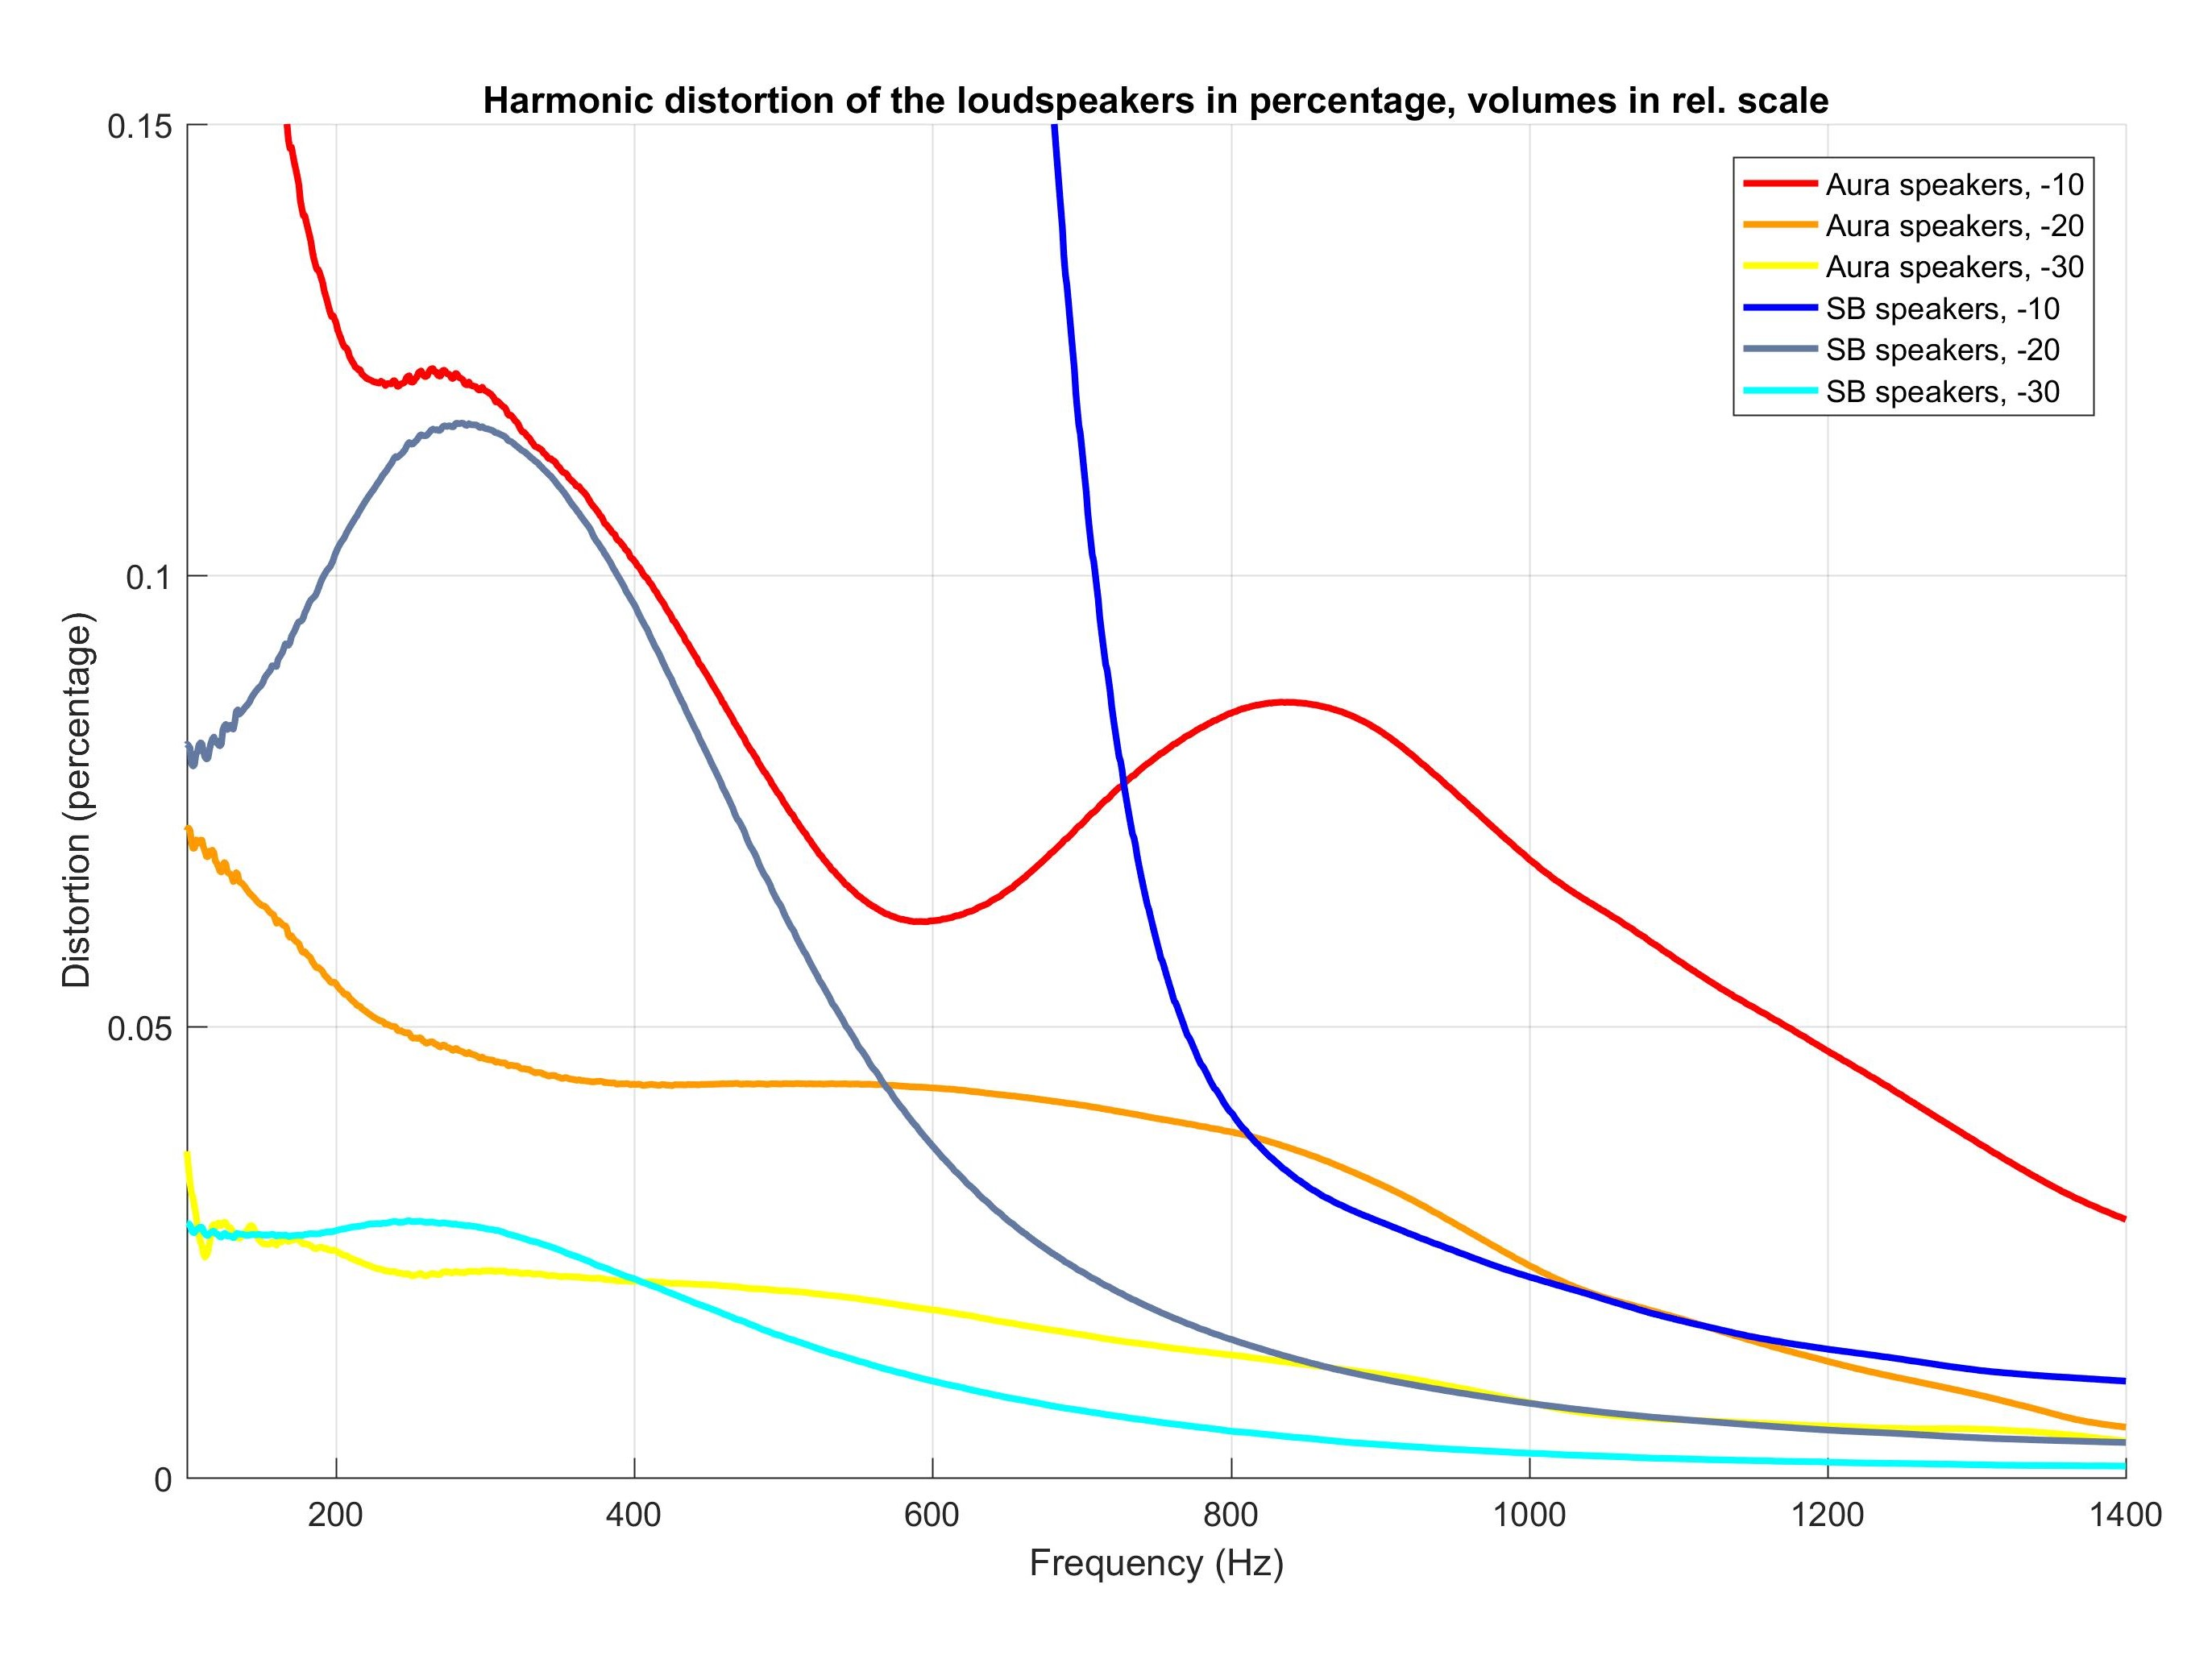
\includegraphics[width=14cm,height=14cm,keepaspectratio]{Figures/harmonicdistortion}
\decoRule
\caption[Harmonic distortion of the two loudspeaker models.]{Harmonic distortion of the two loudspeaker models. Lower is better.}
\label{fig:harmonicdistortion}
\end{figure}

The value in the vertical axis represent the amount of power, in percentage, that ends up generating a nonlinear response. This value was calculated using the formula

\[\frac{\Re\left(H_2(f)\right) + \Re\left(H_3(f)\right)}{\Re\left(H_1(f)\right)}\]

Where $H_1(f)$, $H_2(f)$ and $H_3(f)$ are the first, second and third harmonics of the system. The $\Re$ symbol is the real part of the complex number. The horizontal axis represents the frequency.
\\
This experimental result presented in the graph above is in agreement with what discussed in section \ref{sec:soundgen}. Seeing that the harmonic distortion increases when lowering the frequency is, in fact, what we discussed when talking about harmonic distortions.
\\
\\
As it can be seen from the figure above, higher outputs cause the generation of more nonlinear distortions at all frequencies, even though this effect is more prominent in the lower part of the frequency spectrum ($<500$Hz).
\\
This experiment shows some interesting results. Even though the Aura unit shows lower distortion at low frequencies, crossing over the $750$Hz range the SB speaker appears relatively better, especially when playing sound at lower power levels.
\\
As the reader can see, frequencies over the $1$kHz mark, create very little nonlinearities, especially when using the SB unit, which has a $2\%$ of distortions, even when playing at relatively higher volumes. 
\\
\\
After this analysis, it is possible to determine the unit that better suits our needs for the remainder of this project. As stated in section \ref{Chapter2}, an upper frequency limit was set by the formula \ref{eqn:freqaliasing}, so we already know that the upper bandwidth of the signal will be $2.9$kHz, while we can choose the lower band as we please, trying to stay in the most linear part of the system, since it is the only order of the system that is controlled by the algorithm.
\\
At this point of the project, it was impossible to know the target output level when performing the BACC-RD experiment, but it was clear that playing at lower volumes would have improved the contrast figure.
\\
\\
The model of loudspeakers chosen for the following tests was the SB array. Even though the frequency response of the Aura units is better at low frequencies, the fact that the following experiments could be performed without changing the setup in the room was considered an advantage that overcomes the slightly worse response. If played at an output level (in relative scale) of $-20$ or lower, the harmonic distortion of the SB speakers is $10\%$ at $\tld 300$Hz and it rapidly drops below $5\%$ at $\tld 550$Hz, which can be considered low enough to not disturb the contrast generated by the BACC-RD algorithm (and its later variations).
\\
Moreover the laboratory had a supply of spare loudspeaker units available and an entire, unused, array. It would be later used to reproduce the contrast experiment in the listening room.
\\
The lower frequency limit can be adjusted to best suit our needs, knowing that signal with high powers below the $\tld 300$Hz mark will impact the contrast figure in an heavy way.
\\
Finally, we confronted the SPL generated by each speaker array when all the units in question are playing.
To get this measurement we used all eight the drivers from the Aura unit and speakers 7 to 12 for the SB array. Using the microphone matrix and positioning it at $1$ meter from the center of the array of the speakers used, and outputting the same level, in relative scale, of $-20$, the measured Sound Pressure Level (SPL) was $95.5$dB $\pm0.2$dB for the Aura unit and $94.5$dB $\pm0.2$dB for the SB speakers. This sound level was made by averaging the SPL values of microphones $20, 21, 28, 29$. Each of these measurements was repeated five times.
\\
\\
Now that the properties of the speakers are well known, it is time to start reproducing the results of \parencite{cai_time-domain_2014}.


\section{Applying the BACC-RD method}{}
\label{sec:baccrd}

\subsection{BACC-RD in the simulated environment}{}
\label{subsec:baccrdsim}

In section \ref{sec:simenv} we described the characteristics of the simulated environment. A simulation was needed to debug the BACC algorithm and to quickly change the speakers/microphones/soundzones configuration, in order to get some familiarity with the whole process. Testing the algorithm in a simplified environment greatly sped up the code development by giving the possibility to test the algorithm without having to deal with the underlying hardware. 
\\
\\
Once the IR of the simulated room was proved to be reasonable (figure \ref{fig:simir}), it was given to the BACC algorithm, which would use it to calculate the $R_b$ and $R_d$ terms for equation \ref{eqn:lagrange}. The parameters of the Lagrange maximization problem were set as $\beta = 0.5$ and $\delta = 10^{-6}$ (These are the regularization terms of equation \ref{eqn:lagrange}). The choice of these particular values was made to compare, as we will later see, the eventual contrast figure with the results of \parencite{cai_time-domain_2014}.
\\
At the end of the algorithm, an optimal solution to the Lagrange problem  of equation \ref{eqn:optimization}, in other words, a $w_{BACC}$ filter is returned.

\begin{figure}[H]
\centering
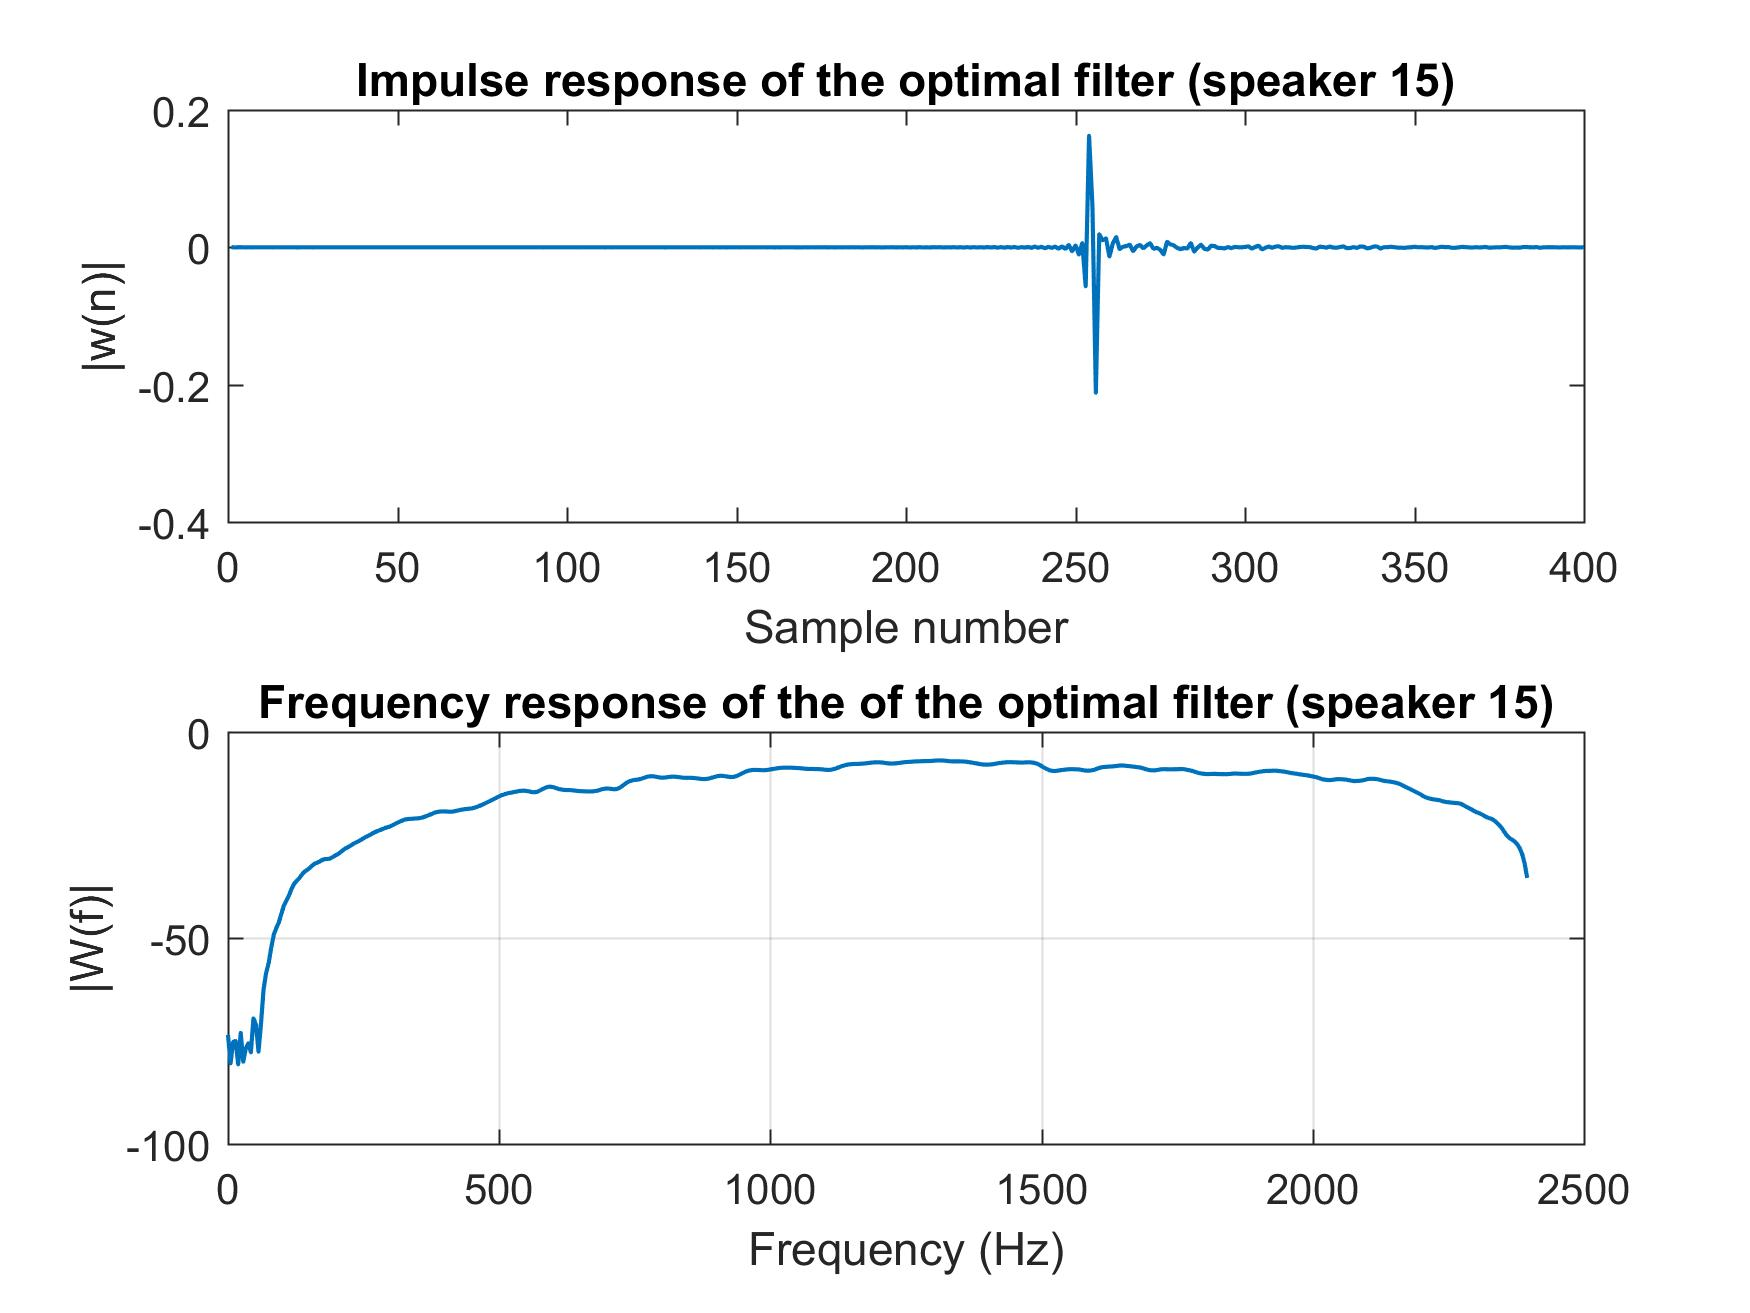
\includegraphics[width=13cm,height=13cm,keepaspectratio]{Figures/ir_fr_w}
\decoRule
\caption[Impulse and frequency response of $w_{BACC}$]{Impulse and Frequency response of $w_{BACC}$.}
\label{fig:ir_fr_w}
\end{figure}

The maximum contrast achievable can vary, even considerably, depending on the particular setup used. In section \ref{subsec:baccvary} we will see how the parameters influence the contrast figure.
\\
\\
Once the IR of the system was estimated, the harmonic distortion of each zone could be compared. This was done by performing the convolution between the simulated IR, the $w_{BACC}$ filter just calculated and a test signal.
\\
The test signal is white noise that has been band-passed in the $[500-2400]$Hz range. There is no particular reason why the frequency range of the signal, at this stage, is that particular one, but this is a similar range to the ones used when performing the experiments in the actual anechoic chamber, hence they can be an useful test bench. Of course the upper limit is limited by the sampling frequency chosen, which was $4800$Hz, but in principle, we could extend both indefinitely.
\\
\\
The algorithm automatically divides the range of the controlled frequencies in a series of equally spaced bins. The central values of these frequency bins will be the control frequencies, the points where the filter will generate the highest contrast, meaning that if we compare the frequency response of the system in the two zones, we will see the biggest excursion between the energy levels of the two ones at those specific control frequencies. By increasing the sampling frequency we are able to shorten the distance between the bins and better control the frequency response of the system, thereby increasing the contrast. A flat frequency response is something desirable because we will output an equal amount of energy in the frequency range of interest, therefore we will not alter the spectral properties of the signal that is being played.

\begin{figure}[H]
\centering
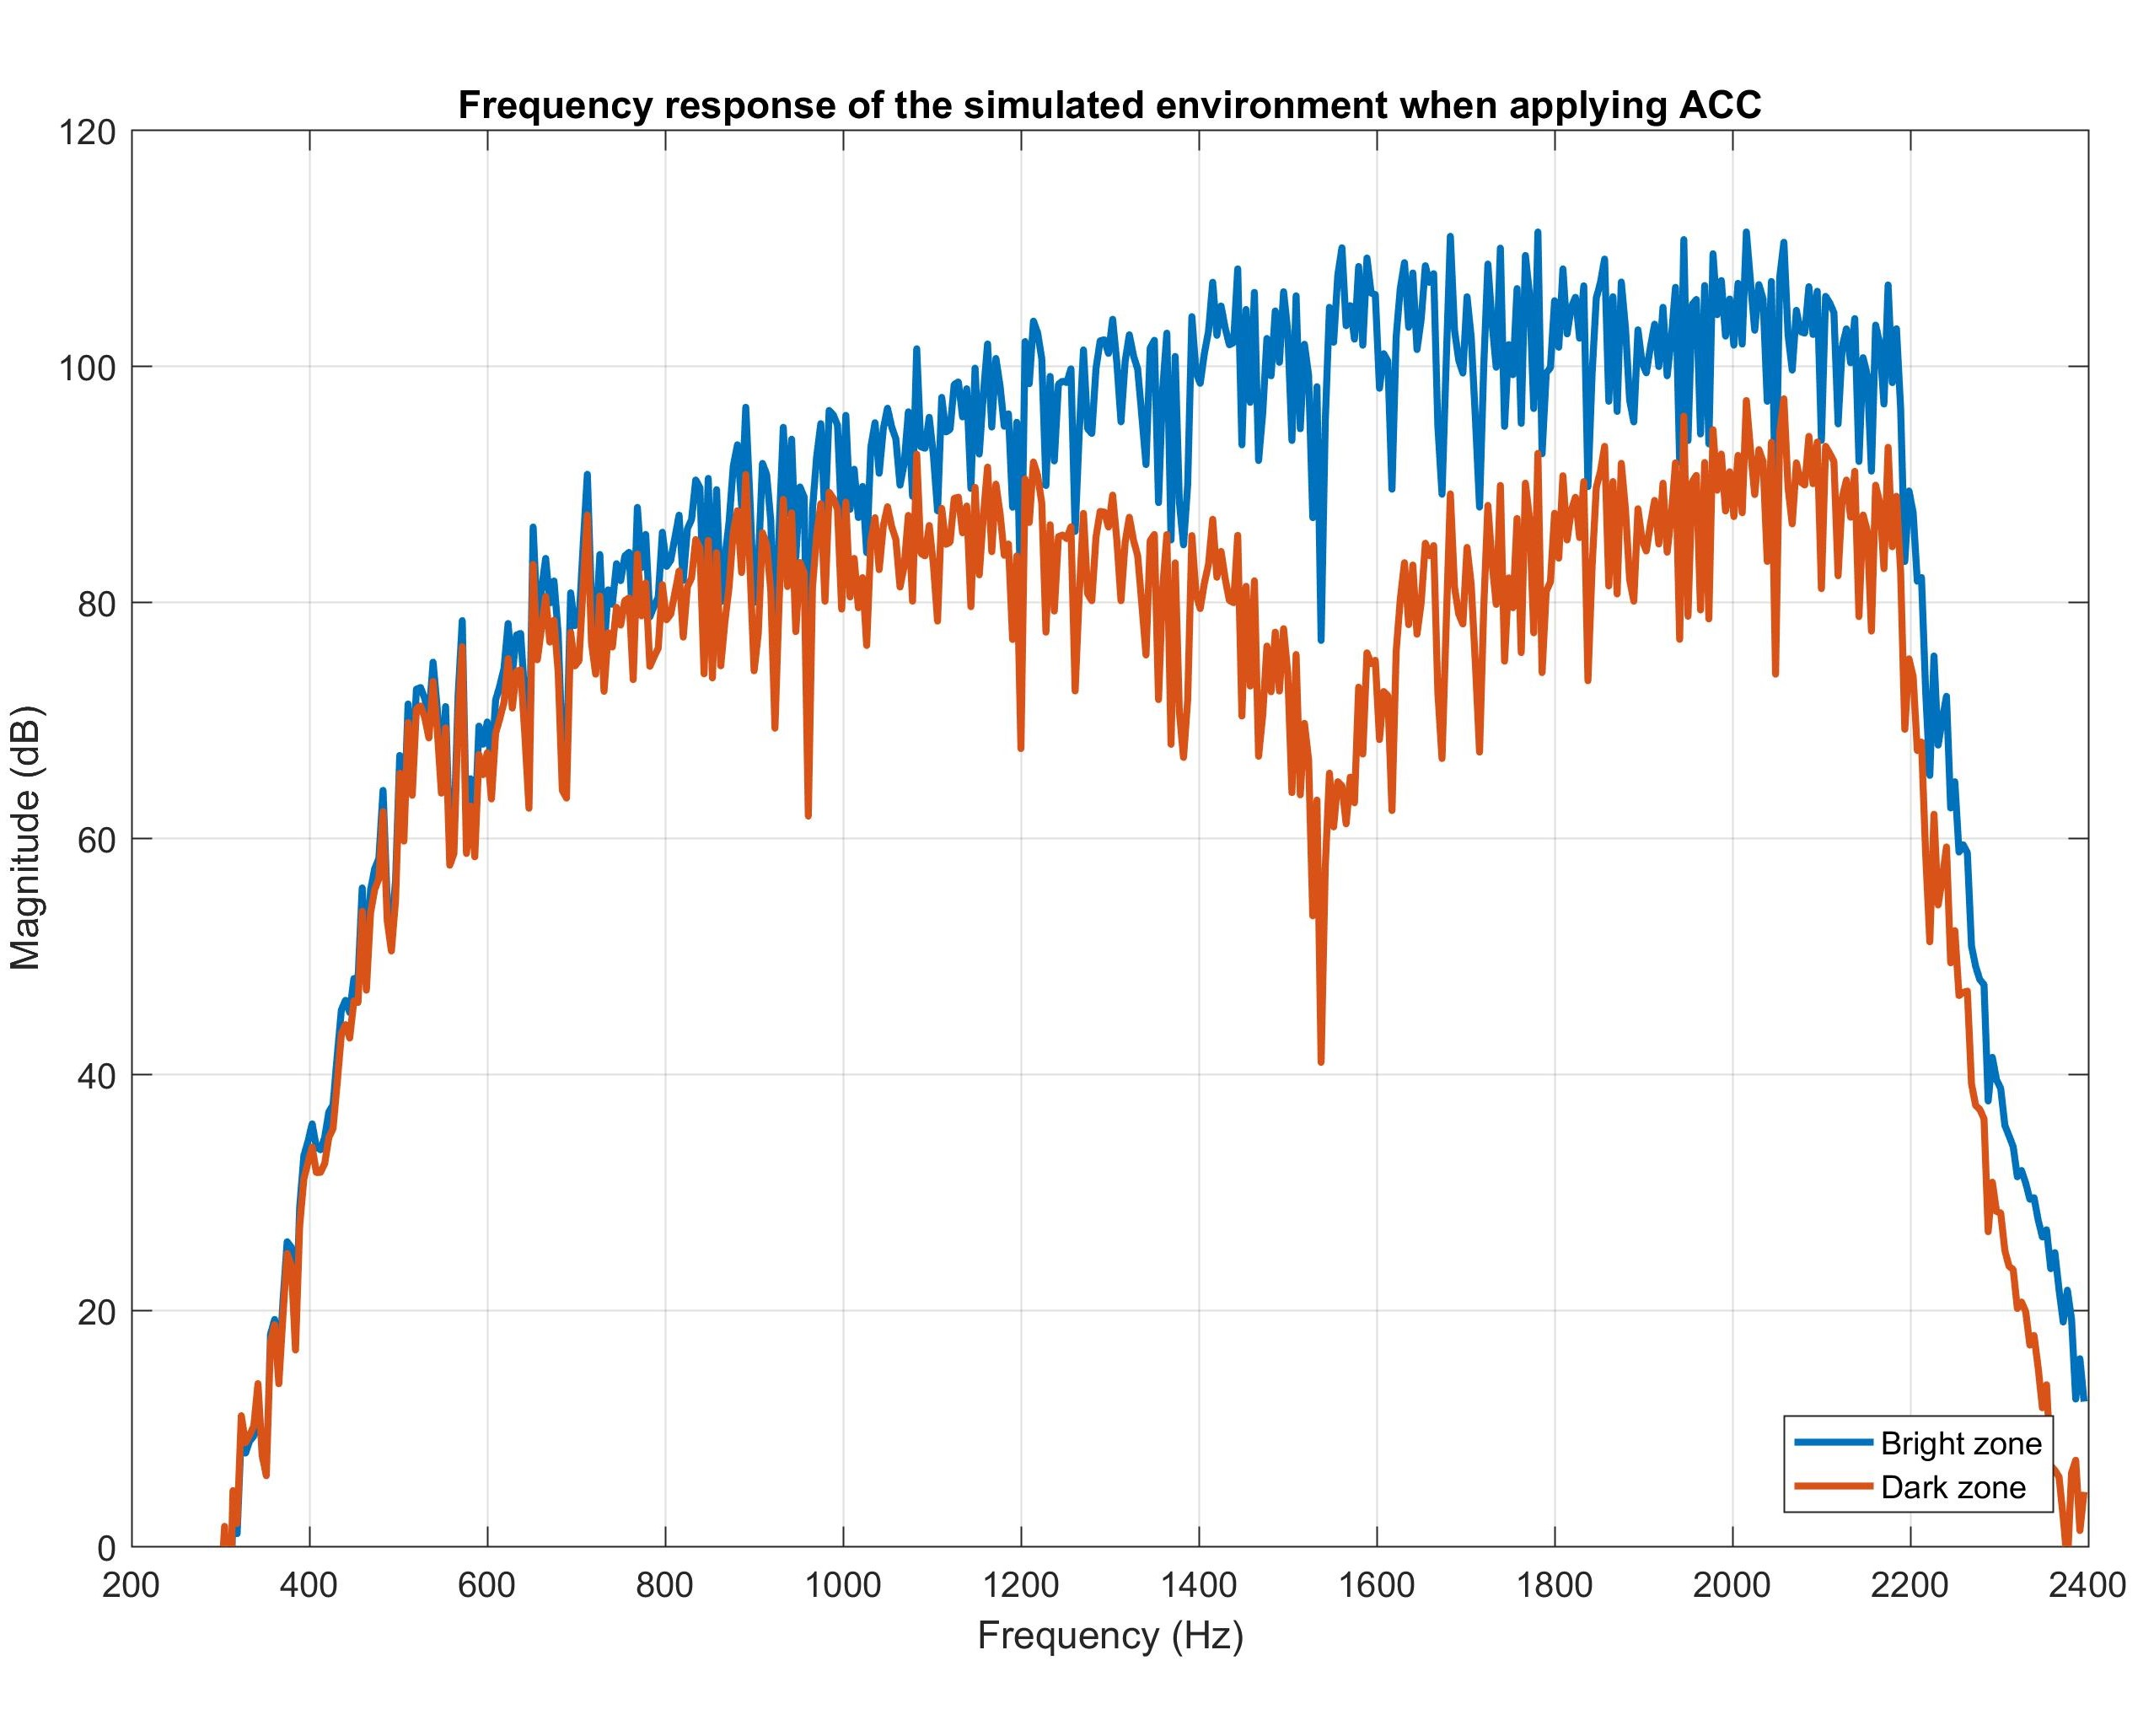
\includegraphics[width=14cm,height=14cm,keepaspectratio]{Figures/contrast_simir}
\decoRule
\caption[Acoustic contrast in the simulated environment.]{Acoustic contrast in the simulated environment. The curves represent the frequency response of the system in the top left microphone of the dark zone and the bottom left microphone of the bright zone from figure \ref{fig:simroom}.}
\label{fig:contrast_simir}
\end{figure}

The theoretical maximum achievable, with the specific room configuration (section \ref{sec:simenv}) and parameters presented above, using the simplified propagation model given by \ref{eqn:green} (which, again, produces the IR in figure \ref{fig:simir}), is $\tld 34.2$dB of acoustic contrast. The contrast figure varies every time we run the algorithm, because of the particular realization of the noise. The sample size generated by running the algorithm multiple times is too small to have a statistical analysis, but after five runs it appears that the contrast diverges from said value by $\pm3$dB.
\\
\\
Now that the algorithm has been tested and we can achieve some acoustic contrast, we could move the experiments in the anechoic chamber.

\subsection{BACC-RD in the anechoic chamber}{}
\label{subsec:baccrdanechoic}

The first step to realize acoustic contrast is to measure the room's IR. This is done outputting the Logsweep function in the frequency range of $[20-20000]$Hz. It is reminded to the reader that the code used for this section was been provided by the AUDIOLAB, later modified in some parts by myself.
\\
The speakers used for this and the rest of the experiments in the anechoic chamber are units 15 to 22 and not units 7 to 12, like the previous test regarding the harmonic distortion of the drivers. This was a deliberate choice, the reasoning behind this is that I originally thought of using different drivers in each of the available array, but the ACC algorithm, promoted higher power outputs coming from some loudspeakers rather than others, accordingly to the positioning of these units with regards to the sound zones. By standing in the bright zone one could clearly tell that the speakers on the right side of the room were playing more loudly than the others. I decided that this effect was unpleasant, so I ended up using the central SB array (units 15 to 22) for the rest of the experiments.
\\
This choice does not alter the results of section \ref{subsec:sbchoosing} in any way, since all the speakers show similar spectral characteristics.
Please refer to figure \ref{fig:anechoicsetup} for more details regarding the position of microphones and speakers used.
\\
\\
As anticipated in subsection \ref{subsec:mics}, the experiments had to be repeated twice, because there was only one microphone stand available. This has to be moved between the two zones. The reader should be aware that this fact introduces a certain degree of uncertainty when estimating the IR of the room. This is because when we are moving the stand from one zone to the other we are changing the response of the system.
\\
For example, let's say after performing the IR estimation with the microphones in the bright zone, we move the stand in the dark one, we are effectively modifying the IR of the room, which was estimated when having a source of reflections (even though small) in the first area, that has now been moved away. This uncertainty cannot be eliminated without adding a second stand with the same shape and working microphones, so that we could measure the IR in both zones at the same time. This, unfortunately, was not an option during the experiments.
\\
It has to be said, though, that this effect has been limited as much possible, by trying to limit the reflection that the various components of the stand introduce, using the specification discussed in subsection \ref{subsec:mics}.
\\
\\
Once the IR of the room is known, we can calculate the correlation matrices $R_b$, $R_d$ and the $RD$ term of equation \ref{eqn:lagrange}.
We have already seen in section \ref{sec:acc} that the filter and IR lengths are a parameter to take into account when calculating the solution to the contrast problem. The increase in length causes an increase in the size of $R_b$, $R_d$ matrices that goes with the square of the sum $M + I$ (filter length plus IR length), moreover this value has to be multiplied for each microphone-speaker pair.
\\
\\
Without going into the specifics of the code, if we decide, for instance, to have an IR and FIR filter lengths of $300$ samples each, using 8 loudspeakers and 4 microphones, we are looking at two matrices ($R_b$, $R_d$) of $5.76 \textbf{x} 10^6$ elements each; If we increase the number of samples to $600$, we will have twice $2.30 \textbf{x} 10^7$ elements. It appears clear how these magnitudes imply a huge amounts of calculations and even with the most powerful hardware available today, it makes finding the optimal ACC filter a rather slow process. For instance, with a 2012 Intel i7 2600K processor with 8GB of DDR3-1333mHz RAM, calculating a $600$ taps $w_{BACC}$ filter takes close to an hour.
\\
This result can vary with the hardware used and I don't exclude that performance improvements in the code might lead to faster results, but it appears clear that finding a balance between the number of samples and the algorithm's performance is very important in order to end up with a reasonable computational time.
\\
\\
In the figure below we can see a closeup of the IR of the anechoic chamber, calculated using microphone 20 and speaker 15. The microphones matrix was positioned in the bright zone.

\begin{figure}[H]
\centering
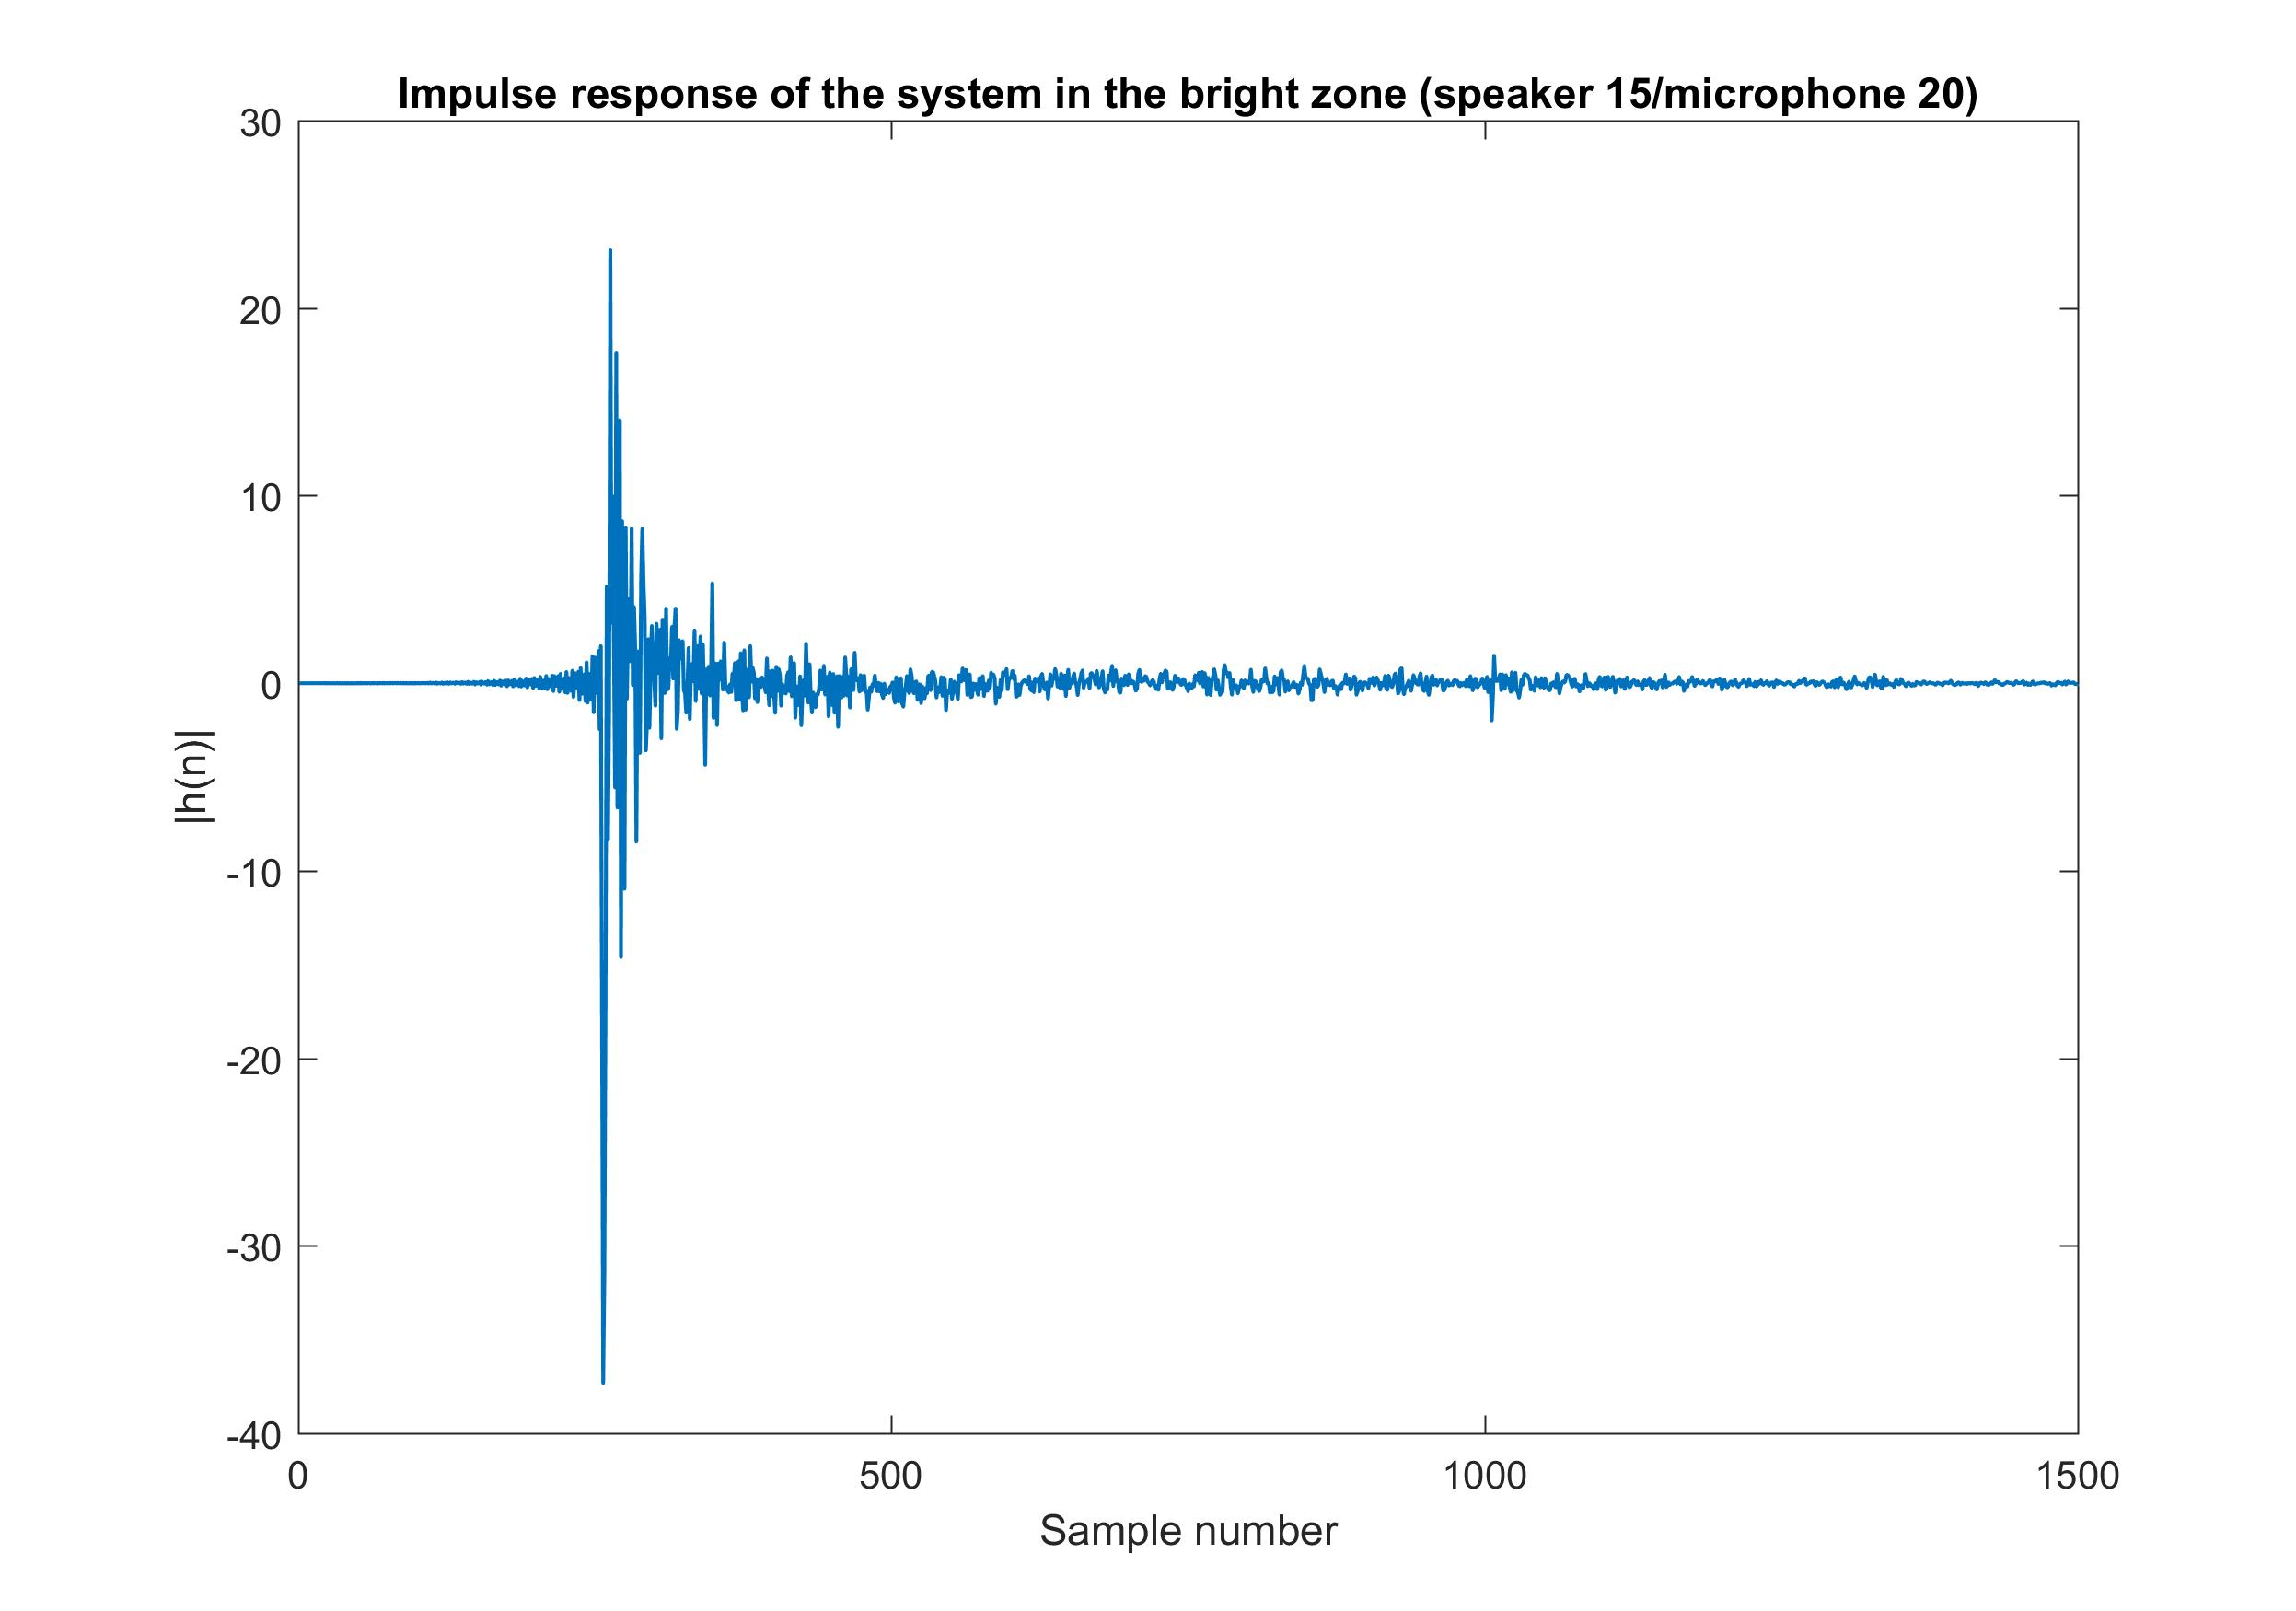
\includegraphics[width=14.5cm,height=14cm,keepaspectratio]{Figures/ir_bright}
\decoRule
\caption[Impulse response of the anechoic chamber]{Closeup of the IR of the system in the anechoic chamber. The measurement starts from the moment the first sound exits the loudspeaker under test. }
\label{fig:ir_bright}
\end{figure}

As already stated, the delay introduced by the hardware is omitted from the graph. The first $\tld 200$ near-zero samples are caused by the acoustic delay, which is the time the soundwaves take to reach the microphones. The measurement was obtained using a Logsweep signal for 10 seconds with $48$kHz as sampling frequency. 
\\
The purpose of having a longer IR is to include more informations regarding the system, so that the $w_{BACC}$ can give us a better acoustic contrast, because it will better "know" the characteristic of the environment it is working into.
\\
From the graph above it appears clear that the IR has a noticeable amount of information well over the first 600 samples, this means that useful information content will have to be excluded in order to be able to calculate a filter in a reasonable amount of time.
\\
\\
Unfortunately, the A/D and D/A converters have a lower limit on the sampling frequency of the input signal, this means that we cannot sample the signal at less than $48$kHz. The sampling frequency determines the total number of samples taken in a given amount of time and by consequence, the length of the IR.
\\
We can overcome this limitation by operating a sample rate conversion on the IR. The conversion is realized by applying a lowpass filter and then decimating the signal, that is, taking a sample every certain number of them, the new sampling frequency is determined by the decimation (or downsampling) rate. The new rate is chosen to be one tenth of the original, so it is $4800$Hz. This of course means that the theoretical upper frequency bound of the system becomes $2400$Hz, due to the Nyquist theorem. This appears to be a reasonable choice, since this value is close to the spacial aliasing limit (determined in section \ref{subsec:mics}) of \tld$2.9$kHz, any frequency above this limit cannot be controlled anyway.
\\
Once the downsampling step is applied, the IR can now better represent the system, because it includes informations about the system relative to a longer interval of time. The trade-off of this technique is that the samples are now taken with a tenth of the original frequency, this means that we will have more time passing between two consecutive record points. This will lead to higher uncertainties, which will inevitably decrease the performance of the algorithm.
\\
Please note that the opposite process has to be applied when testing the filter. Once the algorithm finds $w_{BACC}$, it can be convolved with the test signal, but this output has to be converted (upsampled) back to $48$kHz in order to be sent to the D/A converter (before being amplified and then played).
\\
\\
We have talked about the upper frequency limit, but from section \ref{sec:soundgen} we know that playing sounds at low frequencies generates noticeable harmonic distortions. The widest range the test sound can achieve is $[20-\tld 2400]$Hz, the actual upper limit is rounded by MATLAB's conversion function to the $-3$dB point of the lowpass filter (applied before the decimation) the actual decimated sampler rate is $2376$Hz (which is a loss of 1\%).
\\
Even though the $w$ filter lowest frequency was set to $50$Hz, we will not output much power at that range, because of the harmonic distortion problem.
\\
The last step to complete the analysis is now to generate the test signal, convolve it with the solution found and play it.
\\
\\
At the end of the algorithm, the average acoustic energy (equation \ref{eqn:acousticenergy}) of the two zones is calculated, the filter promises $\tld 29.9$dB of contrast (using equation \ref{eqn:contrast}).
\\
The signal used for the test is generated by applying a bandpass filter to a vector of $4.8\textbf{x}10^6$random elements, corresponding to 10 seconds worth of samples, playing at sampling frequency of $48$kHz. The bandpass filter used is shown below.

\begin{figure}[H]
\centering
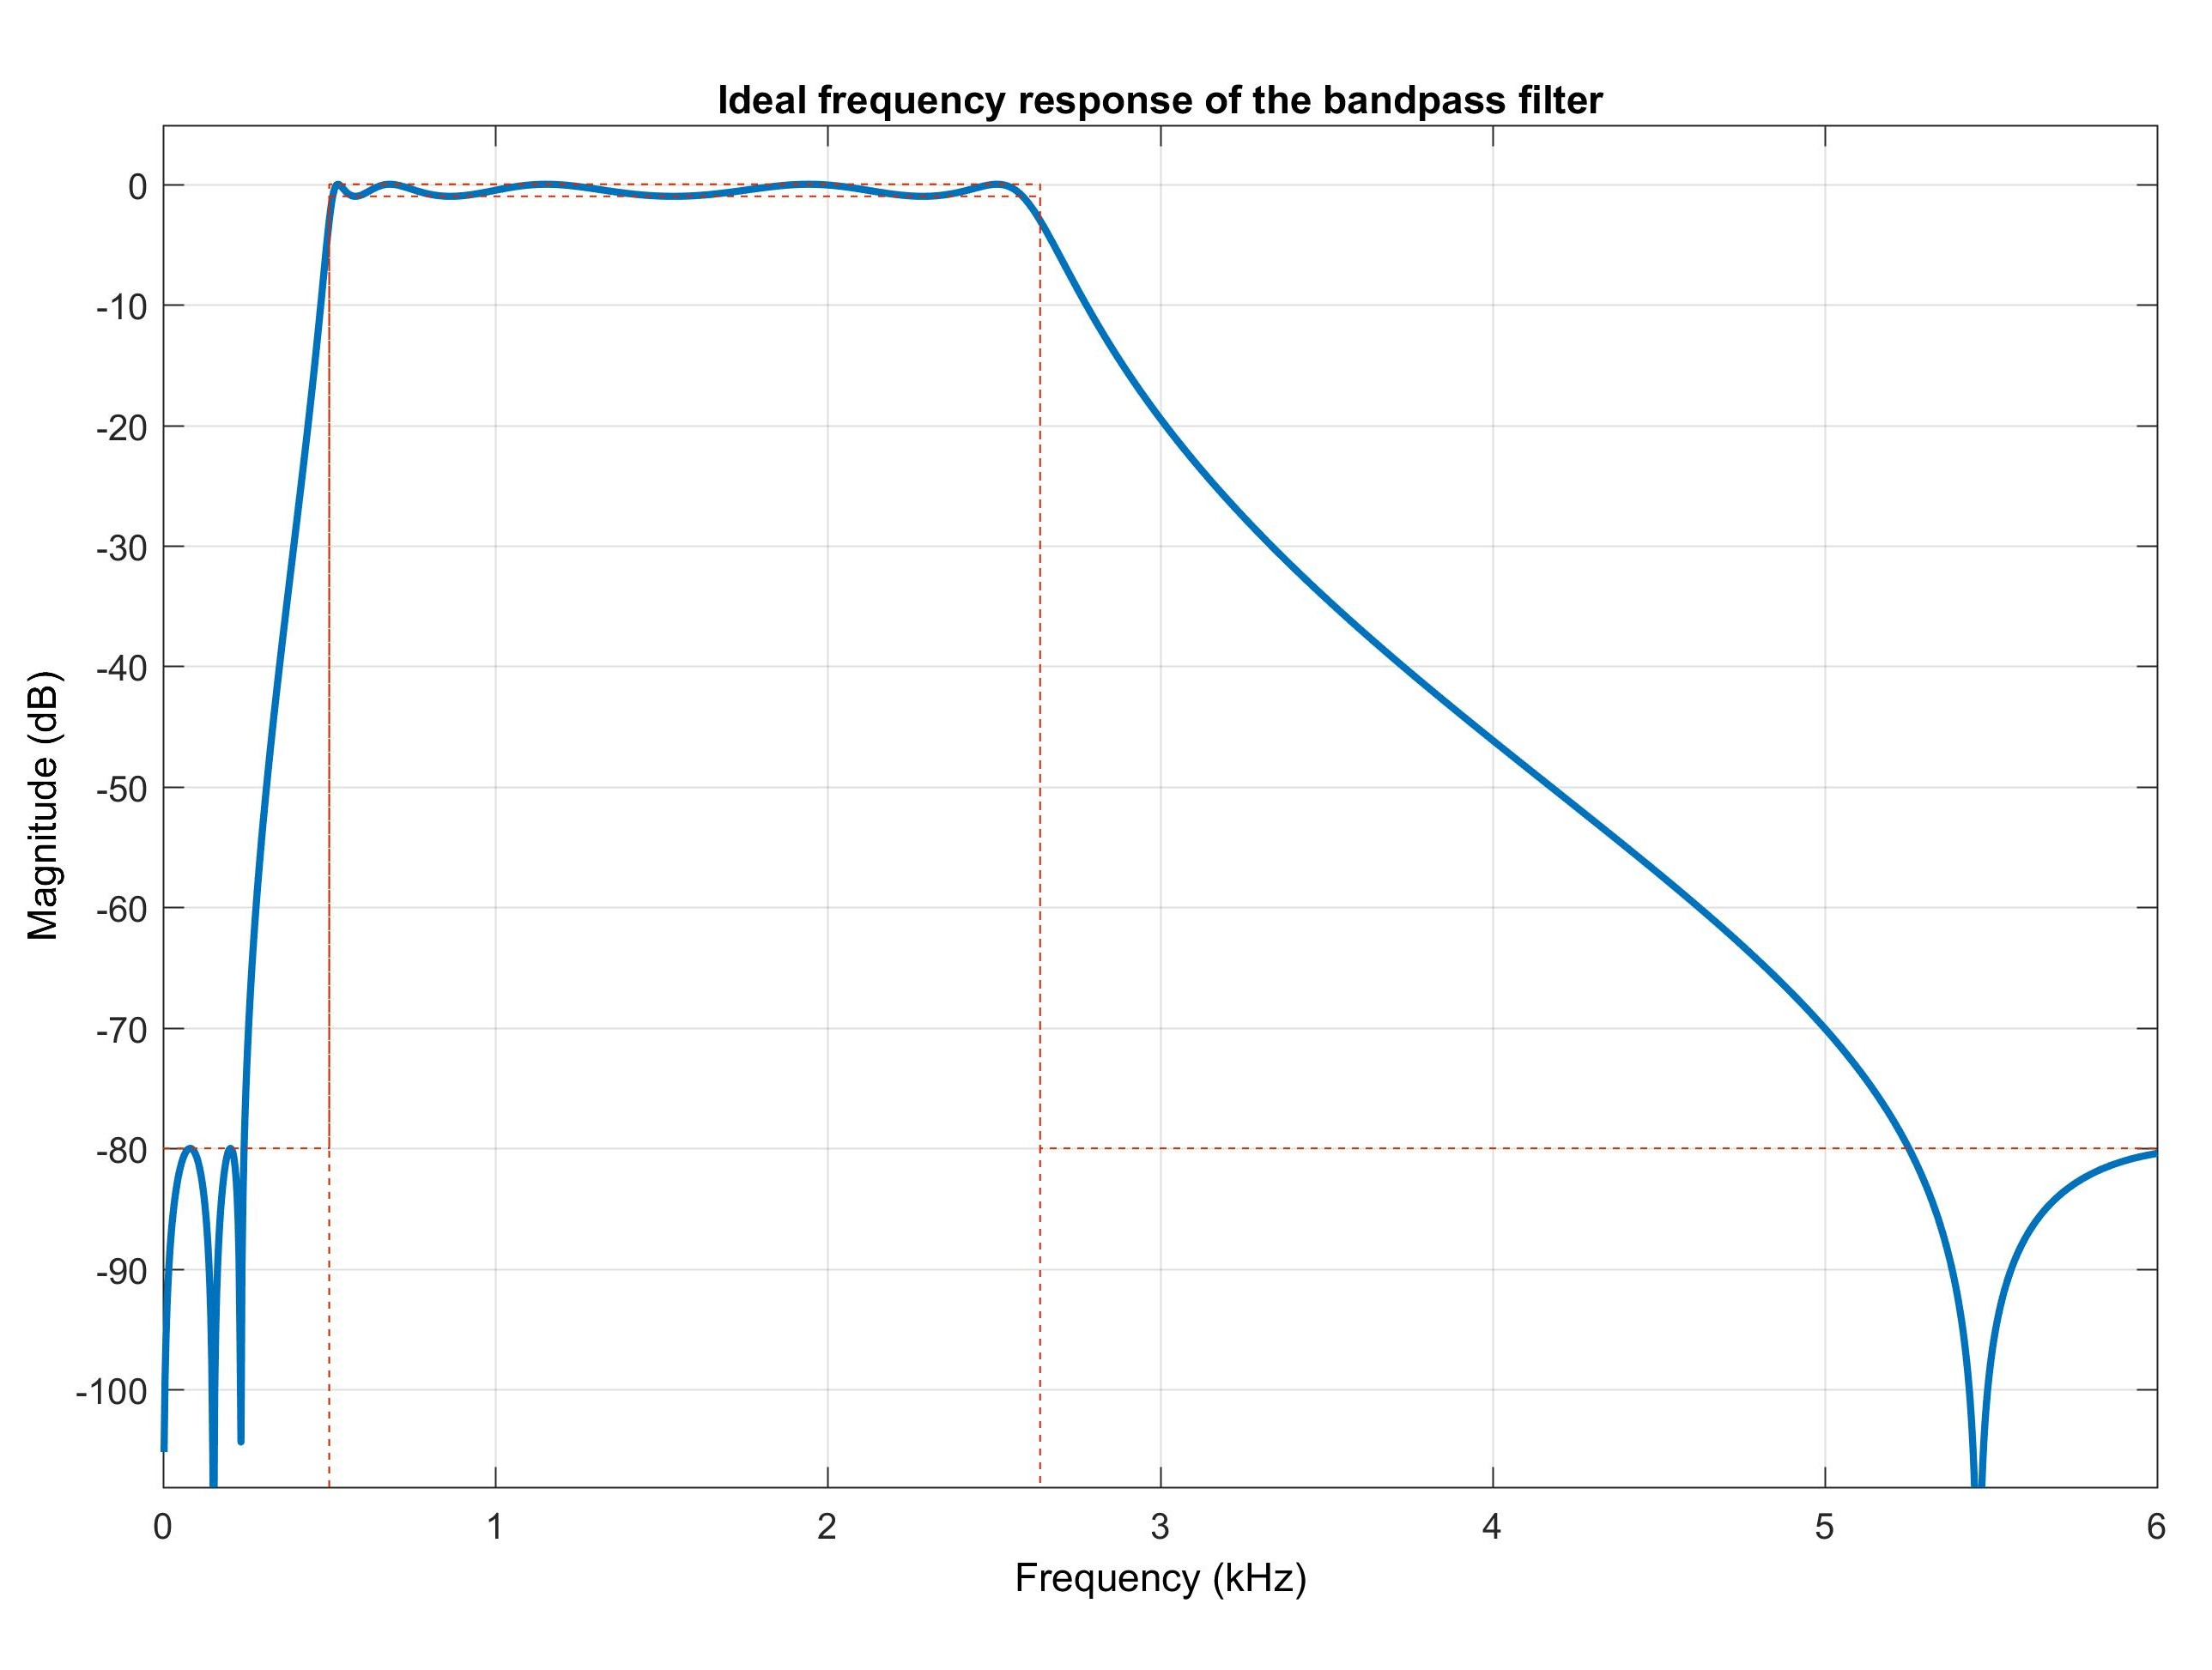
\includegraphics[width=14cm,height=14cm,keepaspectratio]{Figures/noise_bandpass}
\decoRule
\caption[Signal bandpass filter]{Bandpass filter of the test signal.}
\label{fig:noise_bandpass}
\end{figure}

The lower end of the filter is set to $500$Hz, which should generate $\tld 6\%$ of harmonic distortion at $-20$ of relative volume (table \ref{tab:relativescale}), rapidly decreasing at higher frequencies, this means the system behaves in a relatively linear way and the contrast figure doesn't suffer much from the distortions given by the higher harmonics.
\\
The figure below presents two graphs, the first one shows the frequency response of the estimated room transfer function in the bright zone, convolved with both the filter and the bandpass signal, as it will be outputted by the \textbf{first} speaker (number 15). As it can be seen, the power is concentrated in the $[500-\tld2200]$Hz range. Once the gains of the amplifiers will be applied to the signal in figure and the remaining seven loudspeakers (not shown) and outputted, we will record a \textit{linear combination} of such signals. The frequency response of the system (with all the 8 loudspeakers playing), as recorded by microphone 20, is presented in the second graph.

\begin{figure}[H]
\centering
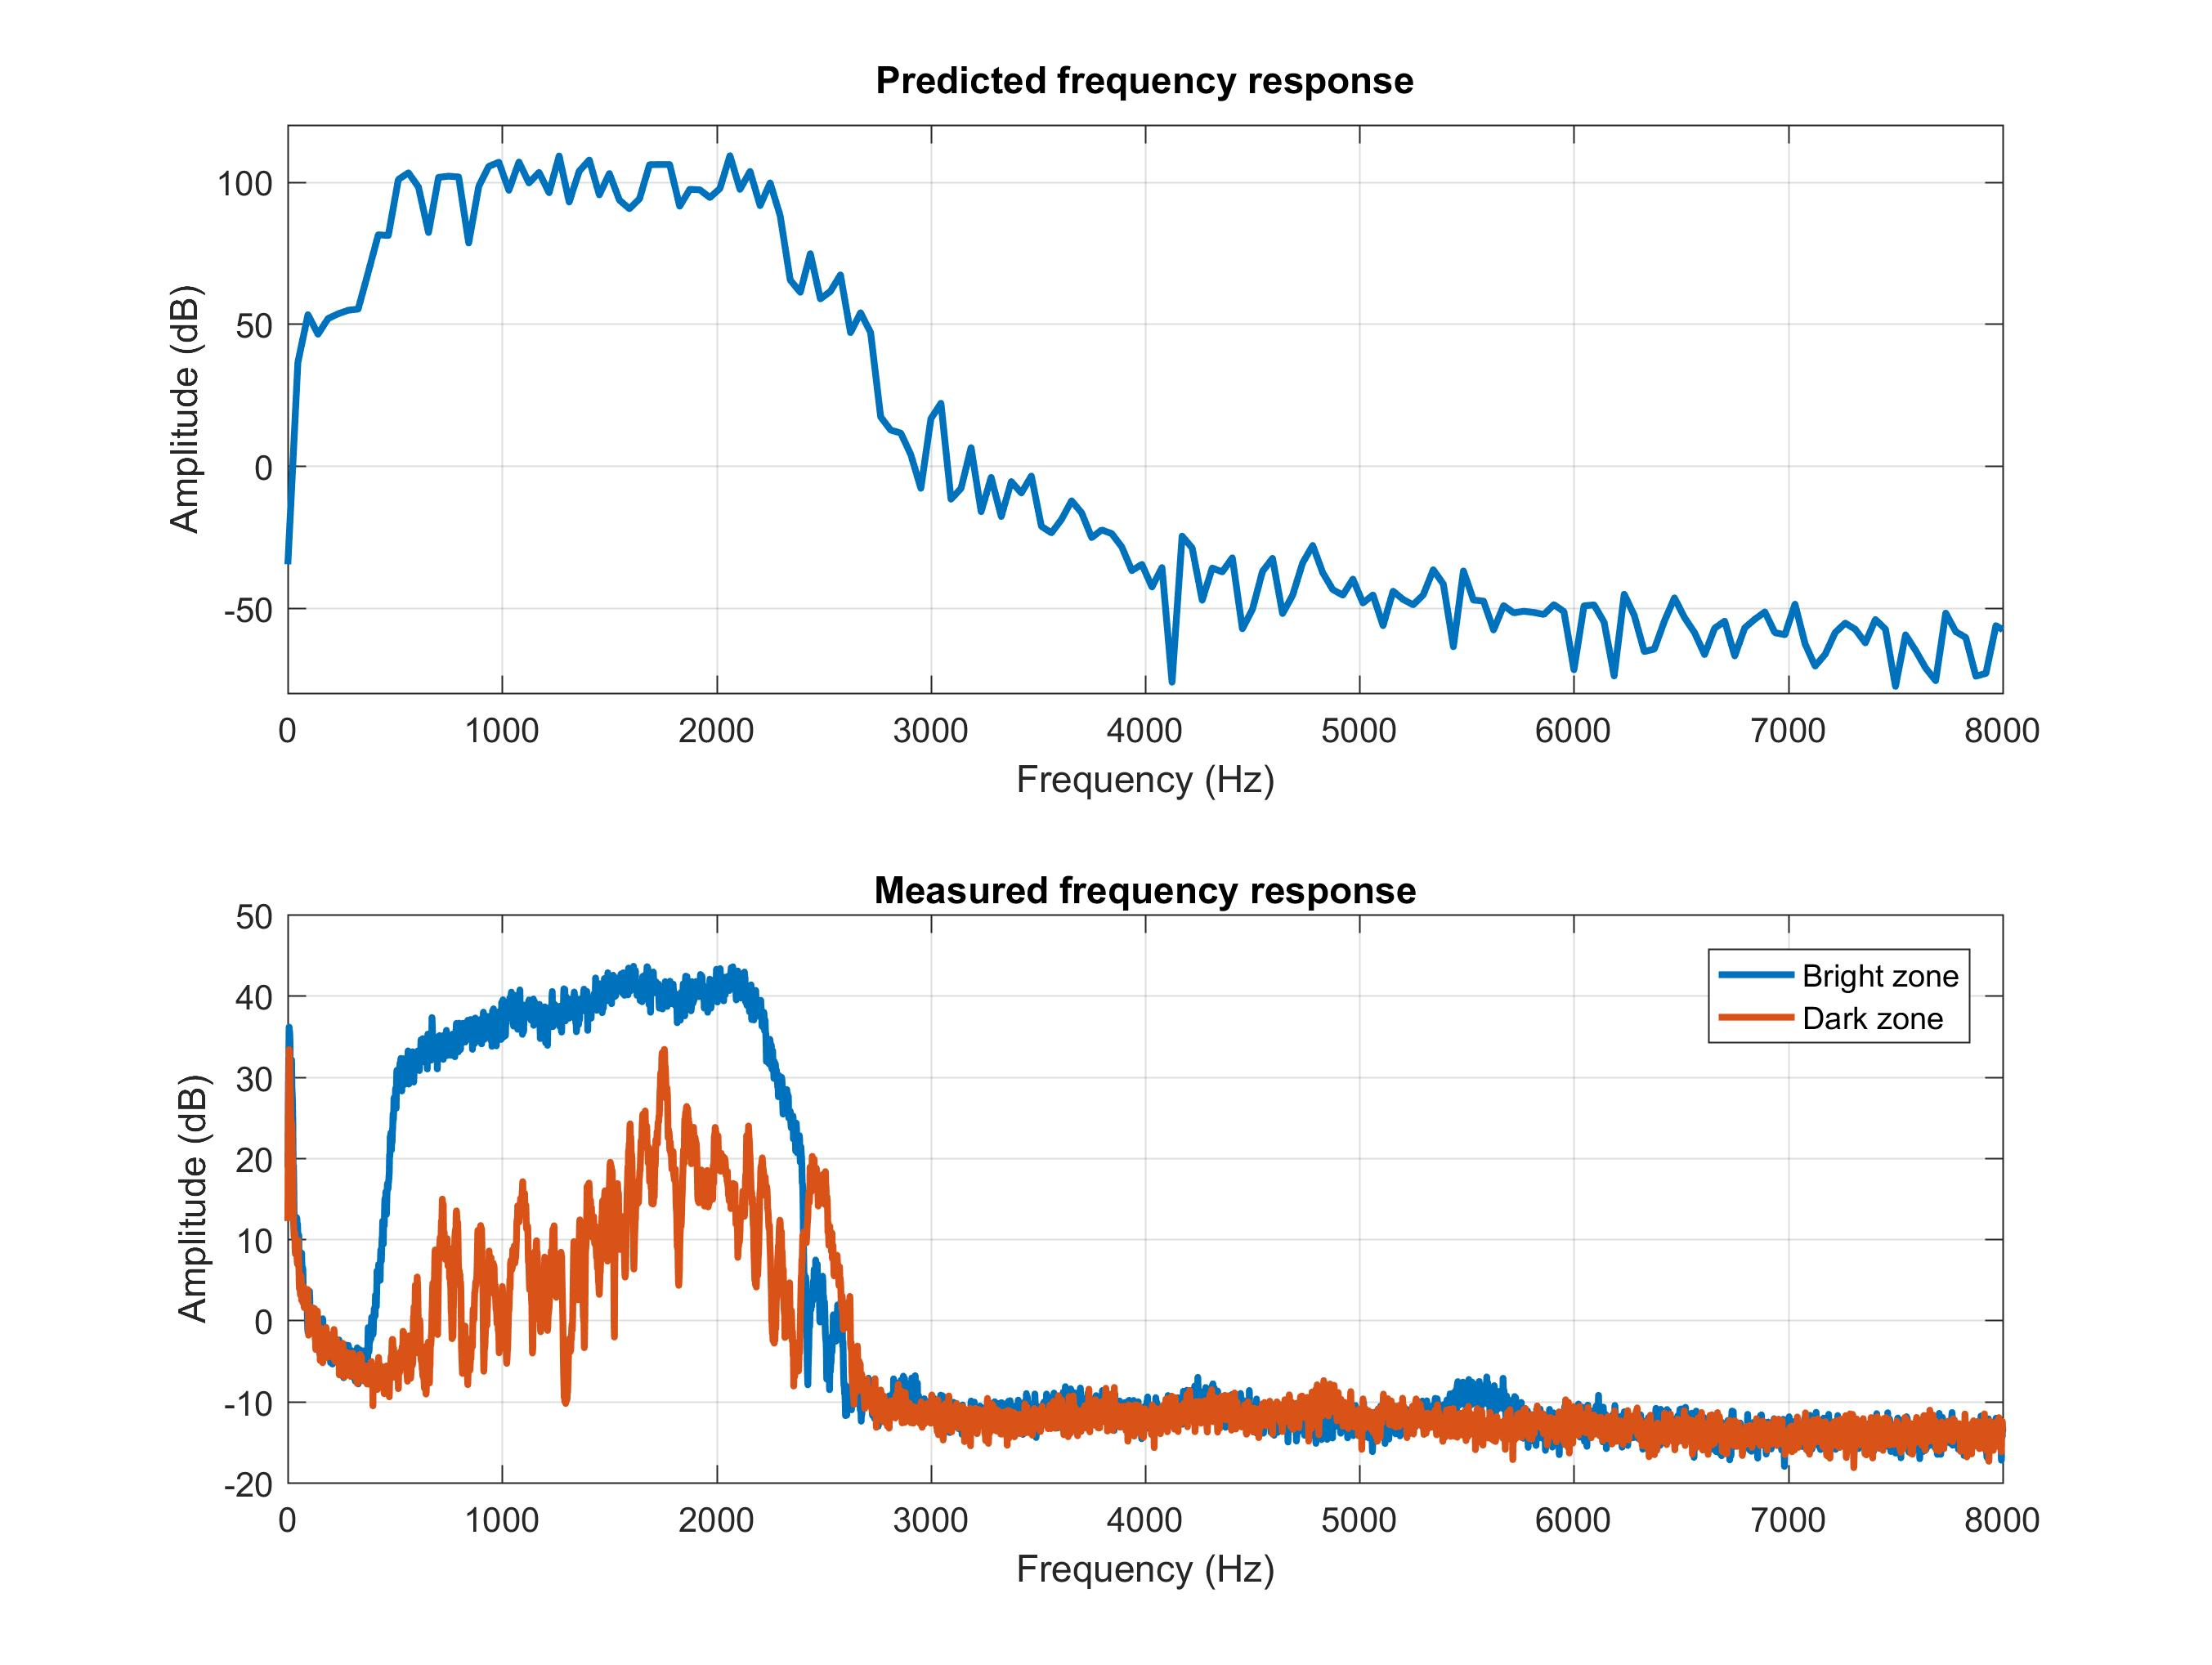
\includegraphics[width=15cm,height=15cm,keepaspectratio]{Figures/fftbacc}
\decoRule
\caption[Frequency response]{Predicted frequency response of the system when considering only the first speaker (first graph) and actual frequency response estimation of the system (linear combination of all eight speakers). Derived using the samples from microphone 20. The estimation was made by using the Fast Fourier Transform.}
\label{fig:fr_multiple}
\end{figure}

The blue line in the second graph represents the frequency content that is found in the bright zone. Please note that the graph is break down by frequencies, this means that the total energy in the zone is the sum of all the contributions from the single frequencies. The orange line in the same graph represents the frequency response of the system in the dark zone.
\\
\\
To get the resulting contrast we applied $10$s of bandpassed white noise, convolved with the BACC filter and recorded the result with four microphones ($20, 21, 28, 29$). These are the innermost microphones, inscribed in an imaginary square centered to the center of the matrix (figure \ref{fig:mics}). We haven't used all the $48$ units because of the increasing size of correlation matrices that this would have meant. As already explained, increasing this size means slower calculations. Using another set of microphones other than the innermost (for instance the outermost) would have changed the spatial aliasing frequency, since the distance between the control points would have increased.
\\
The final band of the system is $[500-\tld 2200]$Hz (an additional 9.1\% away from the Nyquist frequency has been left as bandguard). As previously stated, the signal, in order to be played, had to be upsampled to $48$kHz.
\\
\\
Looking at the second graph, we can see some unexpected behavior from the system. It appears to be some near-DC component in the spectrum, it might be some numerical error generated by the FFT function used, as it doesn't appear to be any low frequency noise when standing at the control point.
\\
The other unforeseen characteristic is that there is a small bias going towards the $2$kHz (and generally the higher) frequencies, the response in the controlled range is flat, in the sense that can be fit in a straight line with little defiation from it, but the \tld$10$dB slope going to the right of the frequency axis was not expected. The algorithm seems to "prefer" the higher frequencies, perhaps because they require less effort to be controlled. This behavior is seen even more prominently when decreasing the value of $\beta$ feed to the algorithm, since $\beta$ is a term that, applied to $RD$ (in equation \ref{eqn:lagrange}) penalizes the control effort.
\\
\\
The acoustic contrast is achieved by comparing the sound pressure levels of the same microphones in the two zones, said microphones have been previously calibrated by using a tone at $1$kHz at a known amplitude.
\\
With the regularization terms $\beta = 0.5$ and $\delta = 10^{-6}$, an output level of $-35$ relative scale (for each speaker) and doing an average of the four microphones used for the measurements, the volume of the noise in the bright zone is $\tld 70.1$dB, while the one in the dark zone is $\tld 45.5$dB. This value appears to be slightly lower than the one presented in table \ref{tab:relativescale} ($4.5$dB less).
\\
This can be attributed to the different kind of signal being outputted (bandpassed white noise, convolved with the BACC filter), rather than the Logsweep chirp.
\\
\\
This leads to a contrast figure of $\tld 24.5$dB, a value close to the theoretical result given by using equation \ref{eqn:contrast}. This is essentially in line with the results of \parencite{cai_time-domain_2014}, done with the same regularization parameters and in a similar frequency range (They present $\tld 27$dB of contrast in a range of $[200-1900]$Hz). Once again, the reader might wonder about the reproducibility of the results. Running the algorithm five times seems to lead to an uncertainty of $\pm 2$dB. I want to stress that affirming this cannot substitute a statistical analysis, which is done with hundreds (or thousands) of data samples. It is encouraging though that the uncertainty seems to be somewhat bounded and in line with the results of the simulated environment. The fact that the time interval used is $10$s gives some robustness against statistical outliers in the noise, hence normalizing the contrast figure.

\subsection{Analysis of the Bacc-RD method using different filter lengths and regularization terms}{}
\label{subsec:baccvary}

Now that we have tested the effectiveness of the algorithm with some real setup we can start asking ourselves some new questions: how do the regularization terms affect the contrast figure?
\\
Similarly, how is the frequency response in the bright zone affected by them? 
\\
How much does the length of the IR affect the performance of the filter?
\\
\\
In order to answer to all of these questions we have to generate a considerable amount of filters obtained using different parameters and test them in sequence inside the anechoic chamber.
\\
The parameters we are going to evaluate are (equation \ref{eqn:lagrange}):
\begin{enumerate}
\item The IR length $I$. The values tested are: $200, 300, 400, 500, 600$.
\item The control effort term $\beta$, with values equal to: $0.1, 0.5$.
\item The regularization term $\delta$, we will choose: $1\text{x}10^{-2}, 1\text{x}10^{-6}$.
\end{enumerate}
The total number of filters tested is $80$, each one of these has been applied twice. The following graphs gives an insight on how do these terms affect the contrast figure.
 
\begin{figure}[H]
\centering
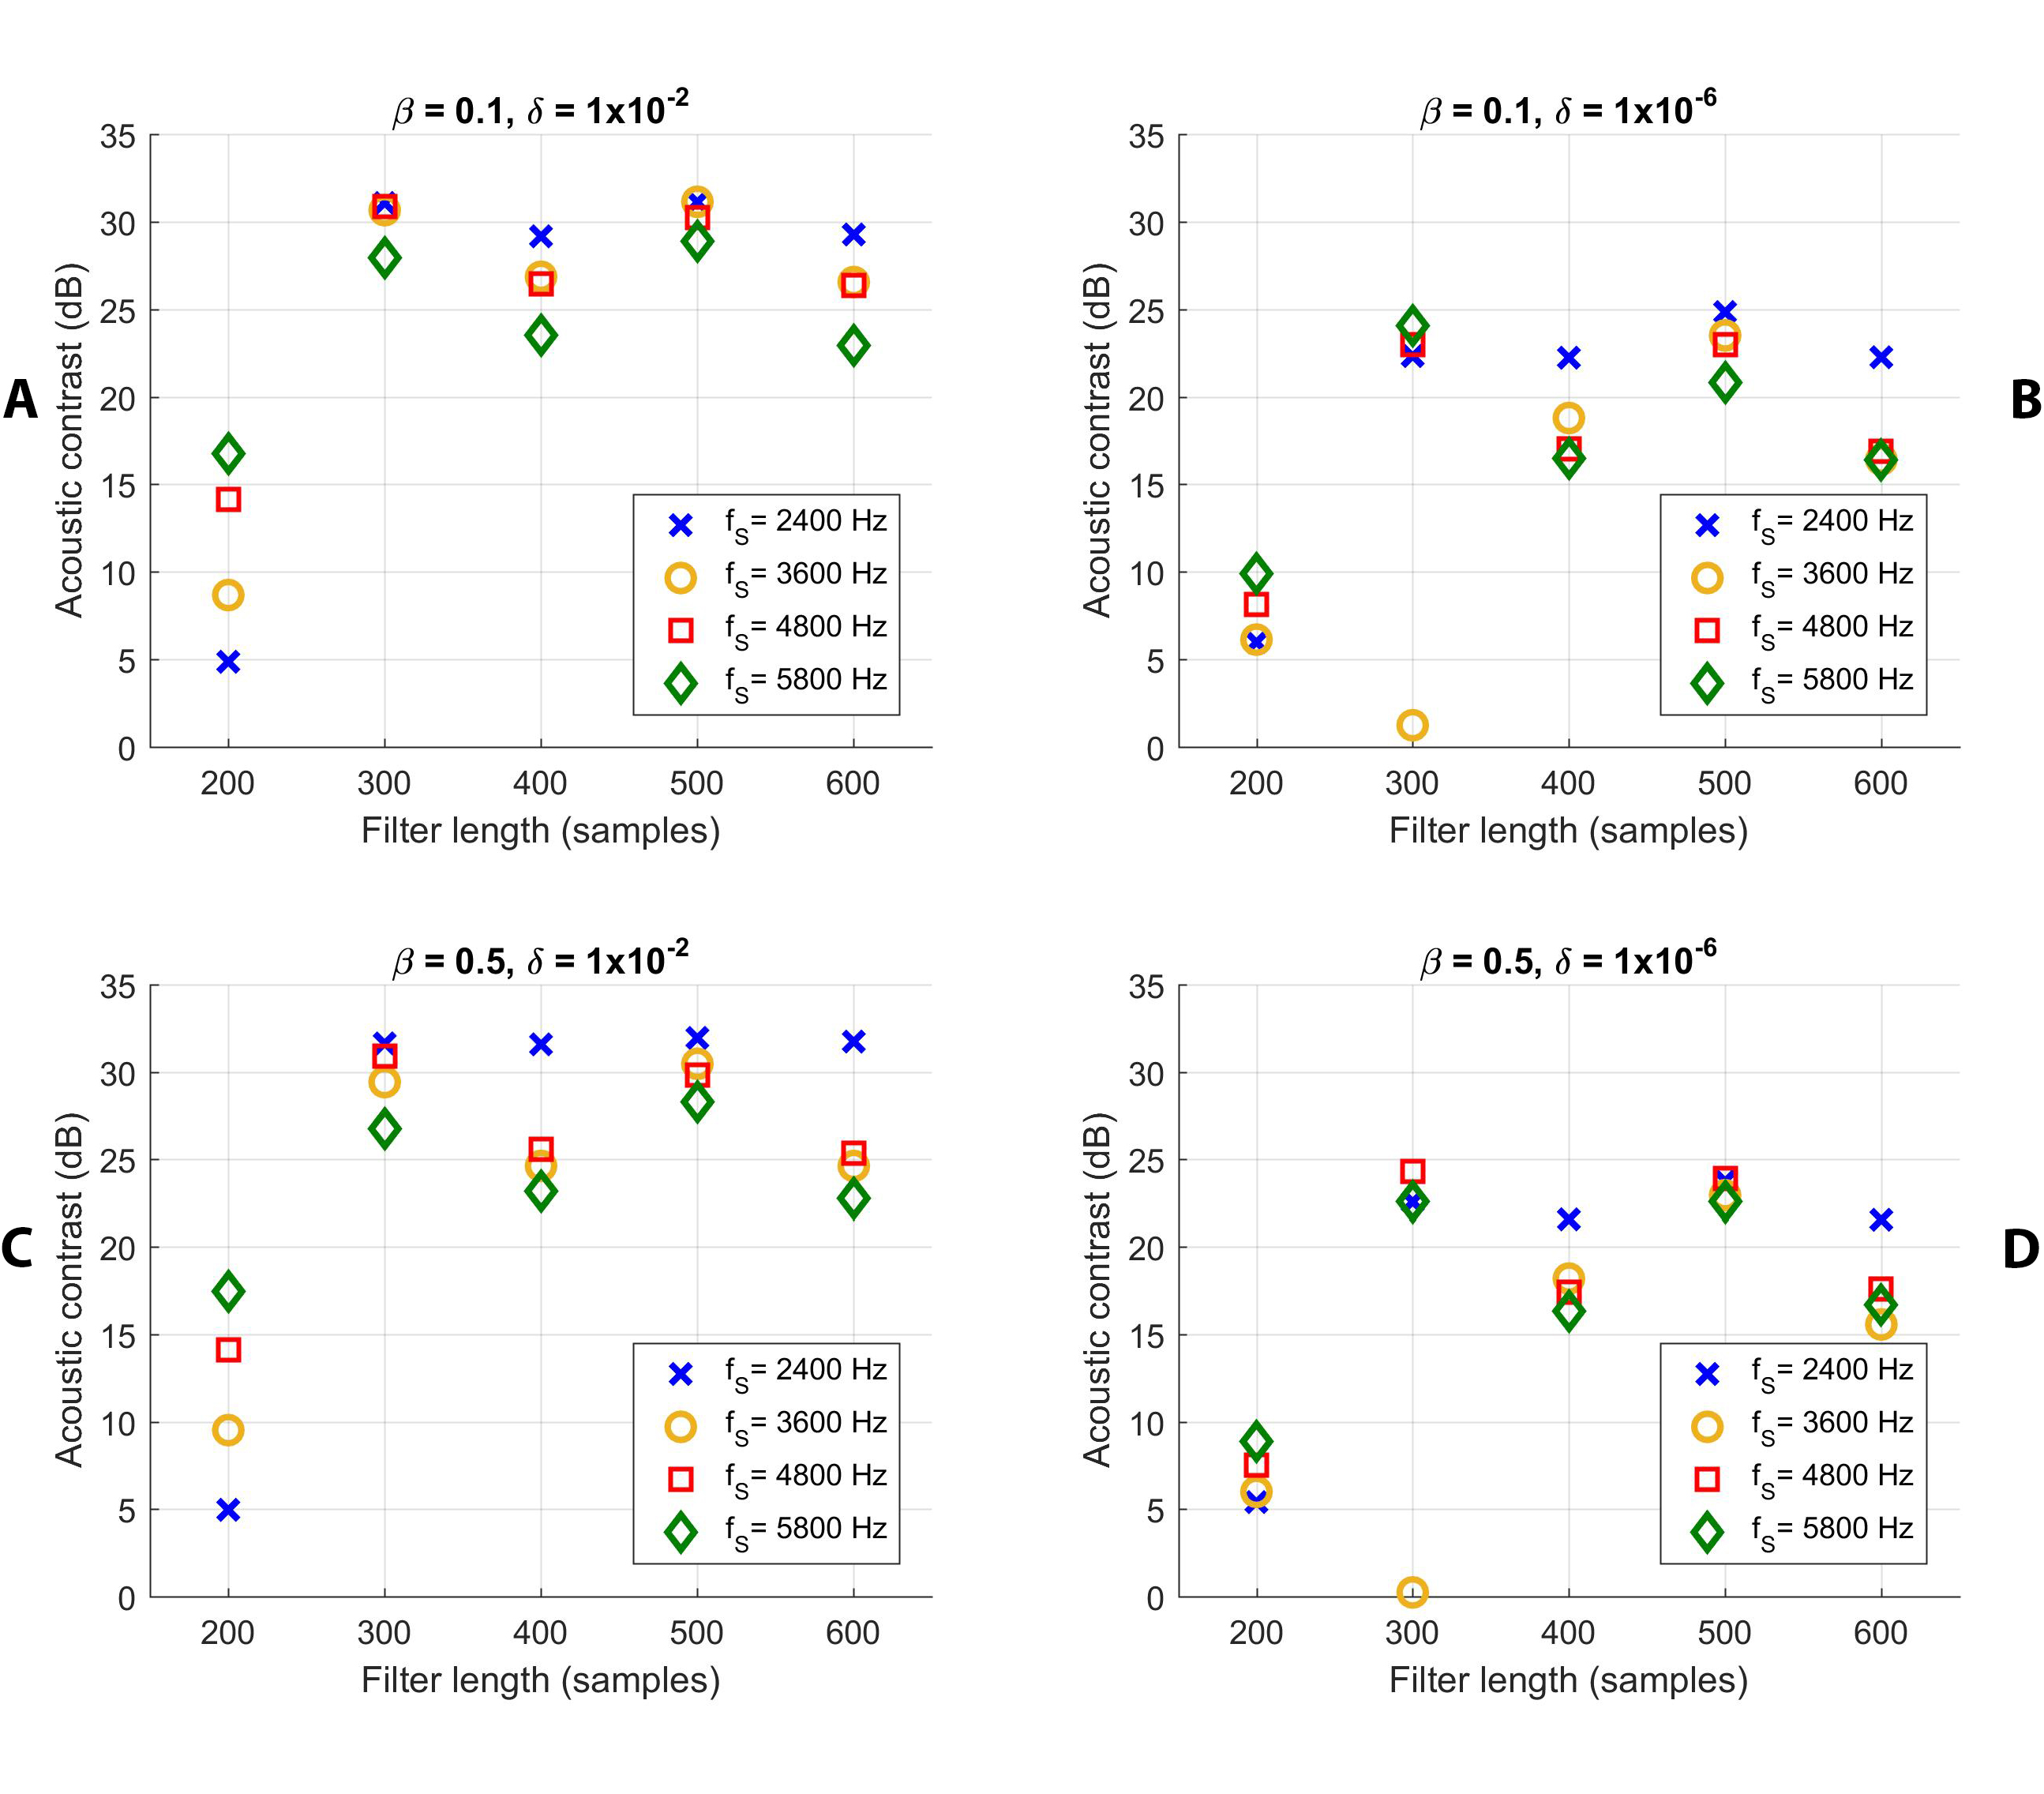
\includegraphics[width=15cm,height=22cm,keepaspectratio]{Figures/comparison_COMP}
\decoRule
\caption[Comprehensive comparison of the filters]{Comparison of 80 filters varying sampling frequency, $\beta, \delta$, filter length.}
\label{fig:comparison1}
\end{figure}

The above figure presents all the $80$ filters used, divided in four categories of $20$, depending on the values of $\beta, \delta$. The four symbols represent the different sampling frequencies used when testing the weights vector calculated using equation \ref{eqn:optimization}. Like the experiments performed in section \ref{subsec:baccrdanechoic}, the original signal, having a sampling frequency of $48$kHz, is downsampled to the value listed as $f_s$ and the upper frequency limit of the test signal is adjusted accordingly. Specifically, the sampling rate is slightly more than double $f_{UP}$, the upper frequency limit, which is determined by the Nyquist theorem, minus a \tld$9\%$ of band guard. The lower frequency bound is still $500$Hz for all of the signals.
\\
The sampling frequencies $f_s$ used are $2400, 3600, 4800, 5800$Hz, while the upper bounds $f_{UP}$ are \tld$1100, 1650, 2200, 2650$Hz, respectively. 
\\
\\
Looking at the figure we can see some patterns. At a length of ($200$samples) for the IR (and the BACC filter, since they are set to have the same value) we see that we have little contrast. This is due to the fact that we are losing too much informations regarding the system by choosing a value that is too small. In fact, if we look at figure \ref{fig:ir_bright}, we see that we have NO information about the system itself, but only some artifacts introduced by the Logsweep signal.In fact, it is very surprising to see that we have some contrast at all. Upon further investigation we can see that the contrast figure itself is artificial. By looking at the filter weights we discover that some loudspeakers are set to play at a louder SPL than others by the algorithm

\begin{figure}[H]
\centering
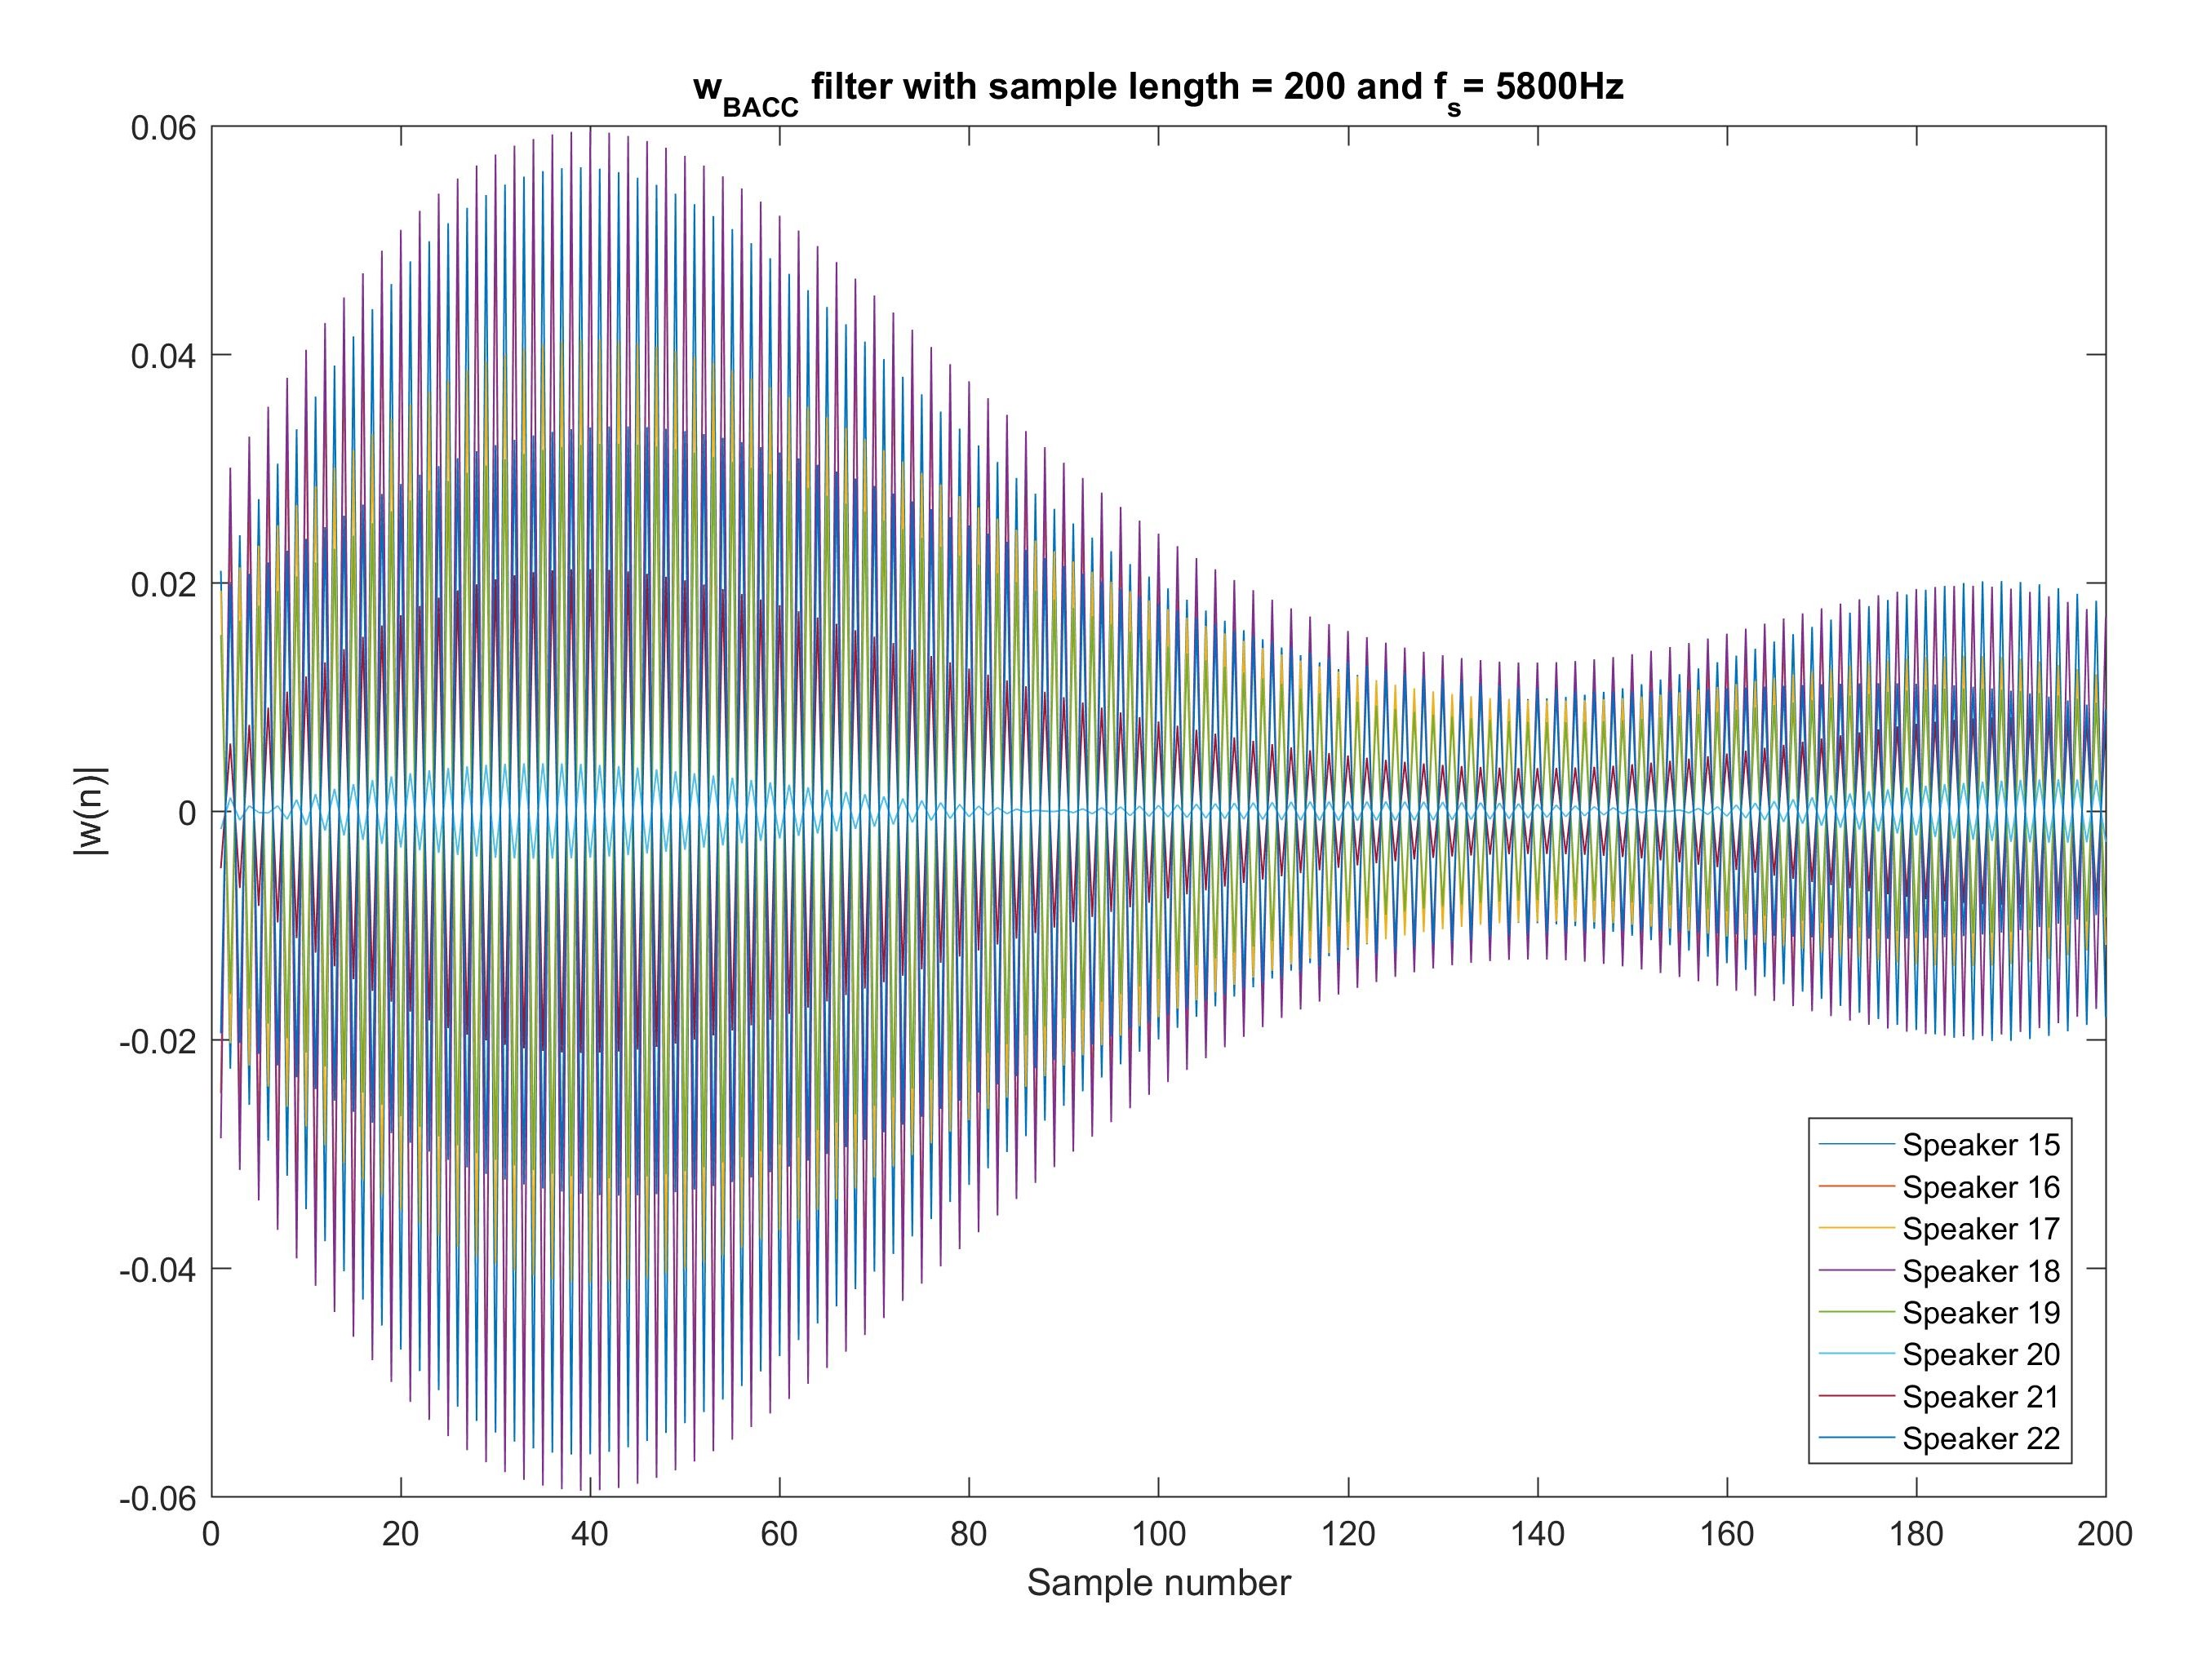
\includegraphics[width=15cm,height=15cm,keepaspectratio]{Figures/filter_strange}
\decoRule
\caption[Superimposed amplitude]{Superimposed amplitude of the BACC filter for all the eight loudspeakers}
\label{fig:filter_strange}
\end{figure}

From the figure it appears that the shape of the weights of the various loudspeakers is similar for all of them, this demonstrates that those filter have been calculated with no actual information content about the system other than the distance between loudspeakers and zones. This is derived indirectly by the samples in the IR that show the artifact coming from the estimation method (Logsweep). The only parameter that changes is the amplitude of the weights, this means that the filter simply increases the sound pressure generated by the driver closer to the bright zone, while the ones adjacent to the dark one are quieter. This difference in SPL is therefore given just by the different propagation of the sound in the room, and it's not the result of destructive interference.
\\
\\
This behavior shows a limitation of the algorithm, the fact that we have no penalization on the control effort, in other words the loudspeakers can be played at whatever volume. To solve this problem it appears necessary to introduce a new constraint on the maximum output allowed to each unit, trying to match all the individual pressure levels. If this technique was to be implemented, the contrast figure when the filter length is too short for the system in question should be (ideally) zero.
\\
\\
Moving away from the edge case and extending the IR length to at least $300$ samples, allows us to design some filters that can contrast sound. We see that lower $f_s$ not only have the highest performances, but also have the best stability in the contrast figure achieved (A, B, C, D). This is because the low sampling frequency (and the smaller frequency band of the test signal) eliminate part of the oscillations of the IR, lowering the overall resolution of the  estimation, having more delay between samples also means that the IR represents a longer time span of the system, giving a more complete characterization. Conversely, even though higher sampling frequencies have a better time resolution, the wider band they use introduces more variance (C), which means that the realization of the noise $\textbf{E}\{AWGN\}$ can alter the results in a more decisive way.
\\
From the graph above we can also see the influence the two parameters $\beta, \delta$ have in the contrast. Comparing (A, C) and (B, D) it appears that $\beta$ has little effect on the contrast itself. This is to be expected, since, as previously explained, $\beta$ controls the "shape" of the frequency response of the system

\begin{figure}[H]
\centering
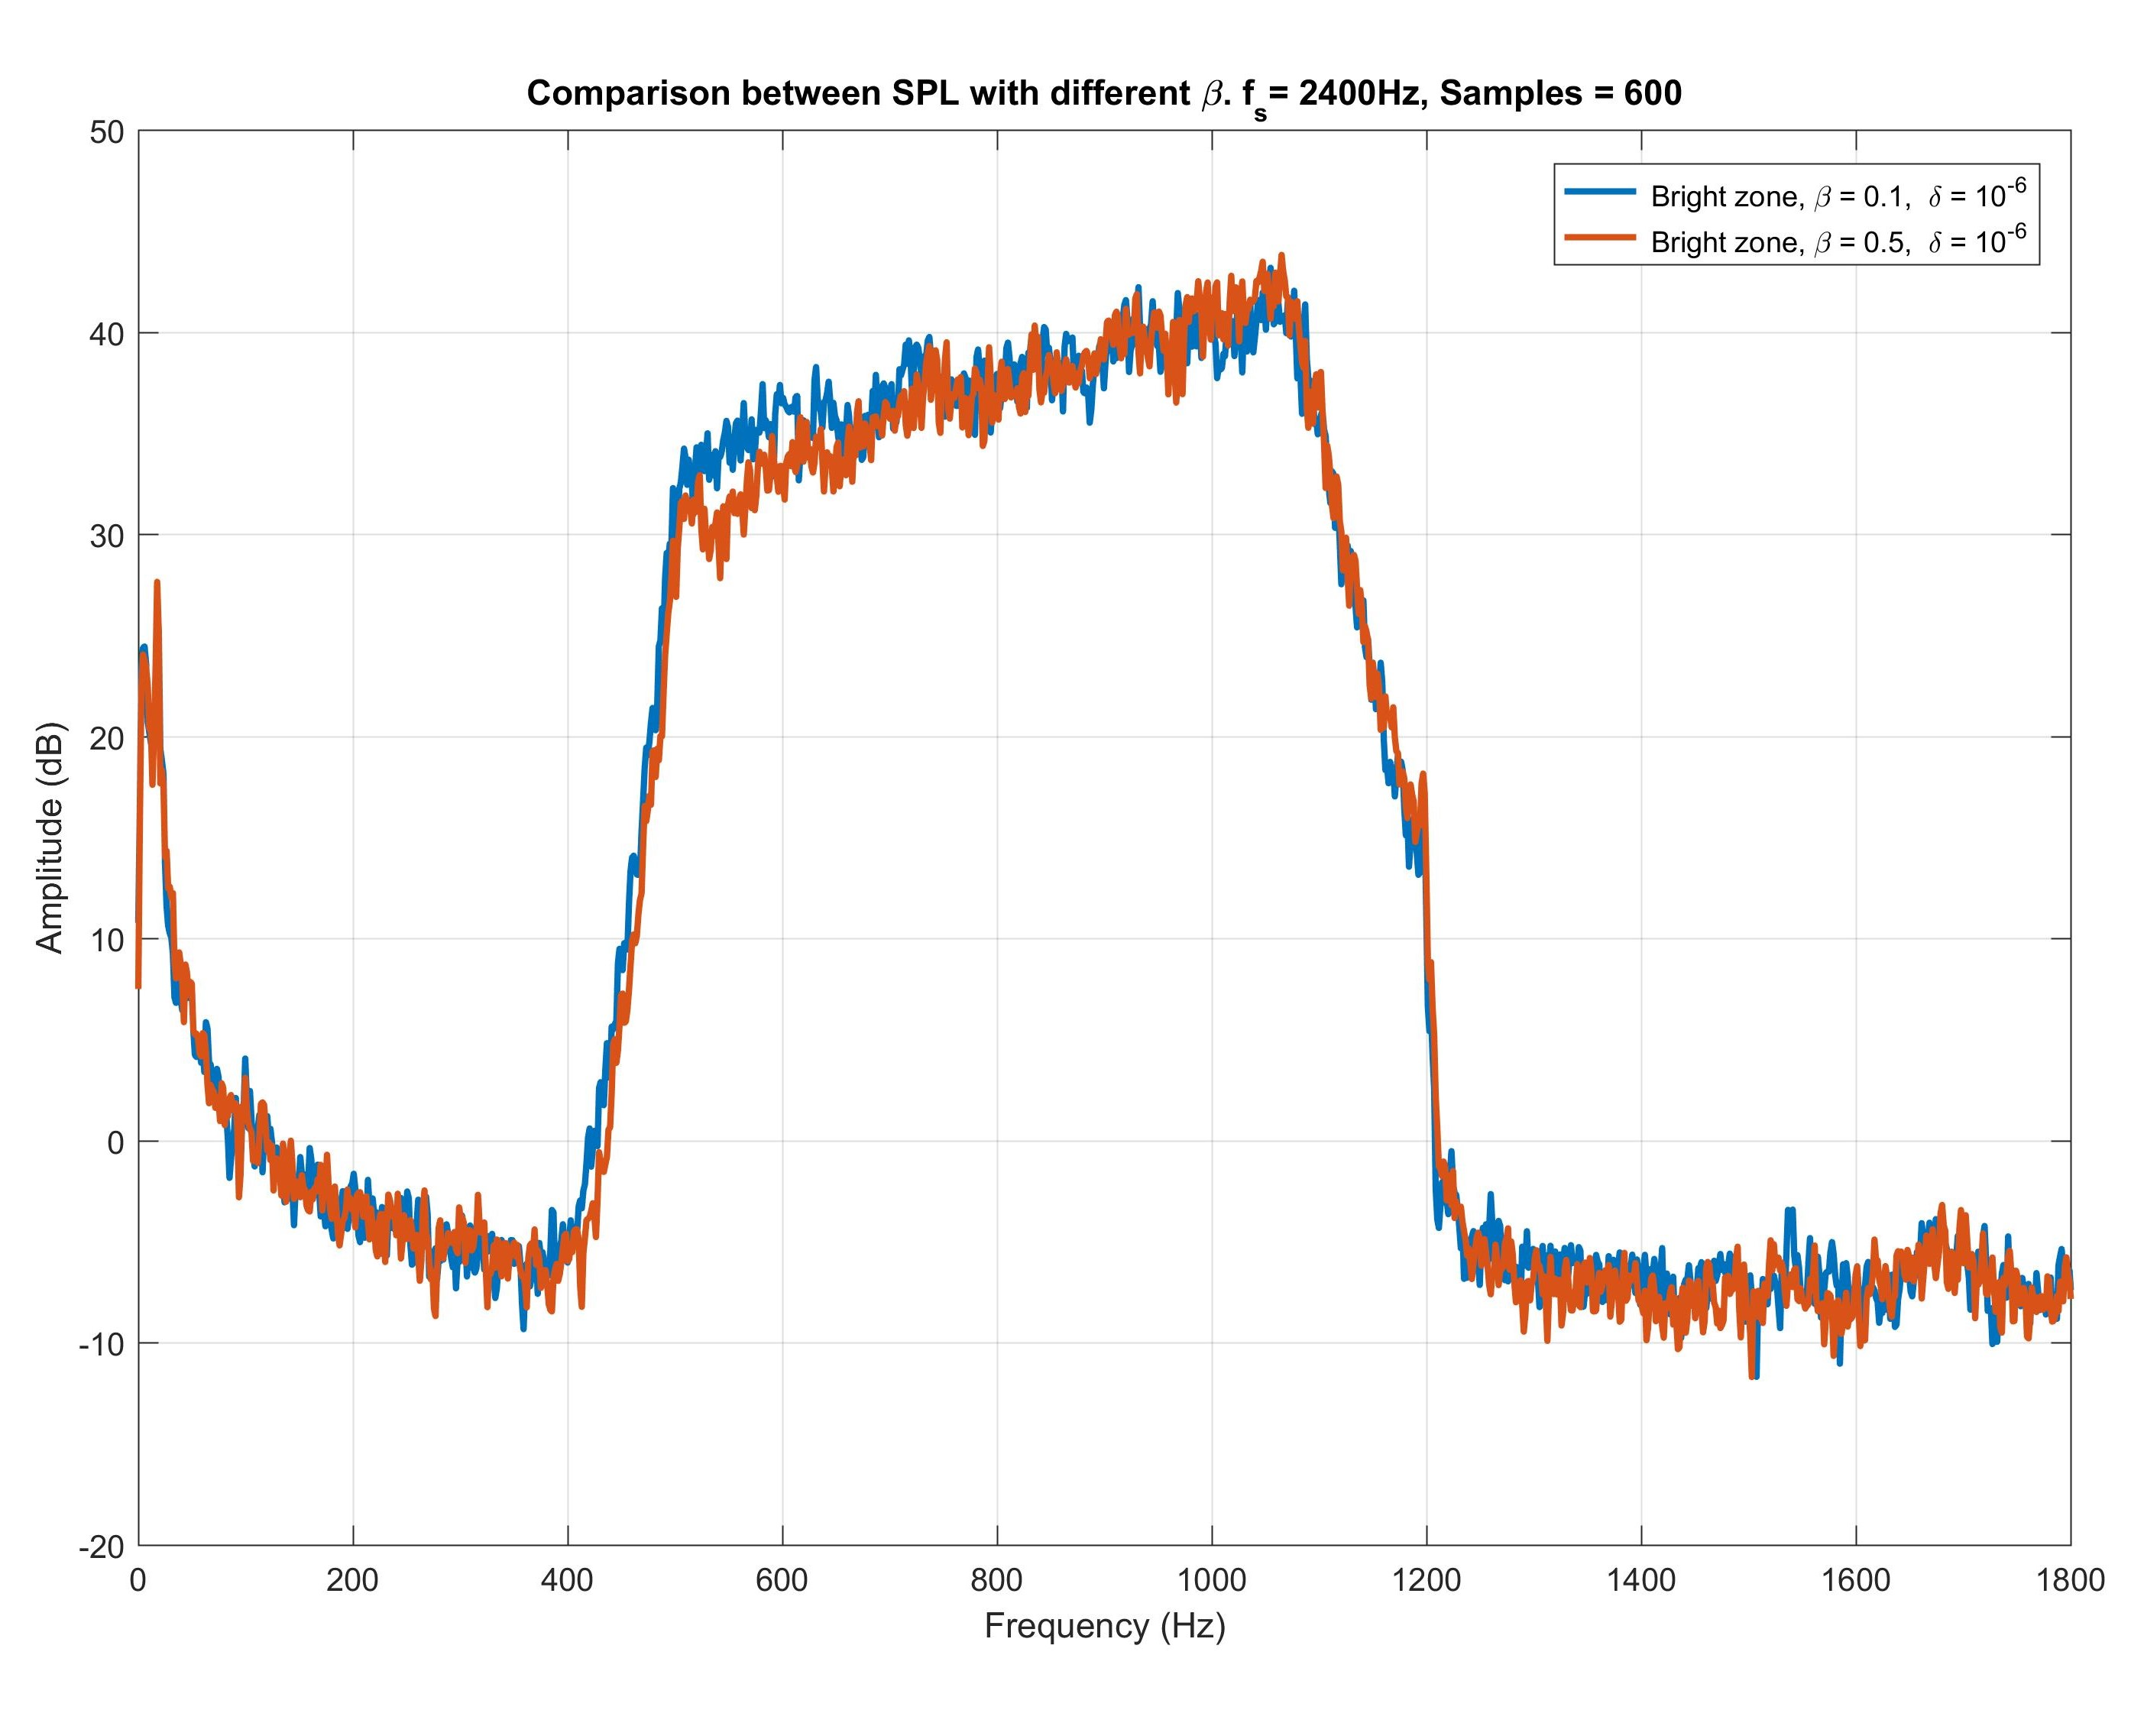
\includegraphics[width=14.5cm,height=15cm,keepaspectratio]{Figures/filter_25vs65}
\decoRule
\caption[FFT filters same delta]{FFT of the recording of microphone 20 for two filters with different $\beta$.}
\label{fig:filter_25vs65}
\end{figure}

The figure shows the Fourier Transform of two filter (both with $f_s = 2400$Hz and $600$ samples) as recorded by microphone 20, positioned in the bright zone (graphs B and D). We can see that the frequency response of the system is very similar in both cases, and in general not affected by $\beta$. What is effected instead is the slope of the frequency response in the range of interest, this is because a lower value of $\beta$ penalizes less the alteration of the shape of the FR, so the algorithm tends to maximize contrast in the higher part of the spectrum, therefore by skewing the response. The contrast figure of the two filter is $22.2\pm2$dB for the first one (blue line) and $21.8\pm2$dB for the second (orange line).
\\
\\
The value of $\delta$ instead affects the contrast figure as shown in graphs (A, B) and (C, D). This is because $\delta$ determines the error bound, the maximum deviation an element of the correlation matrices $R_b, R_d$ is allowed to have before being discarded for the calculation of the maximum eigenvalue in equation \ref{eqn:lagrange}. A lower bound implies an higher sensitivity of the algorithm. 

\begin{figure}[H]
\centering
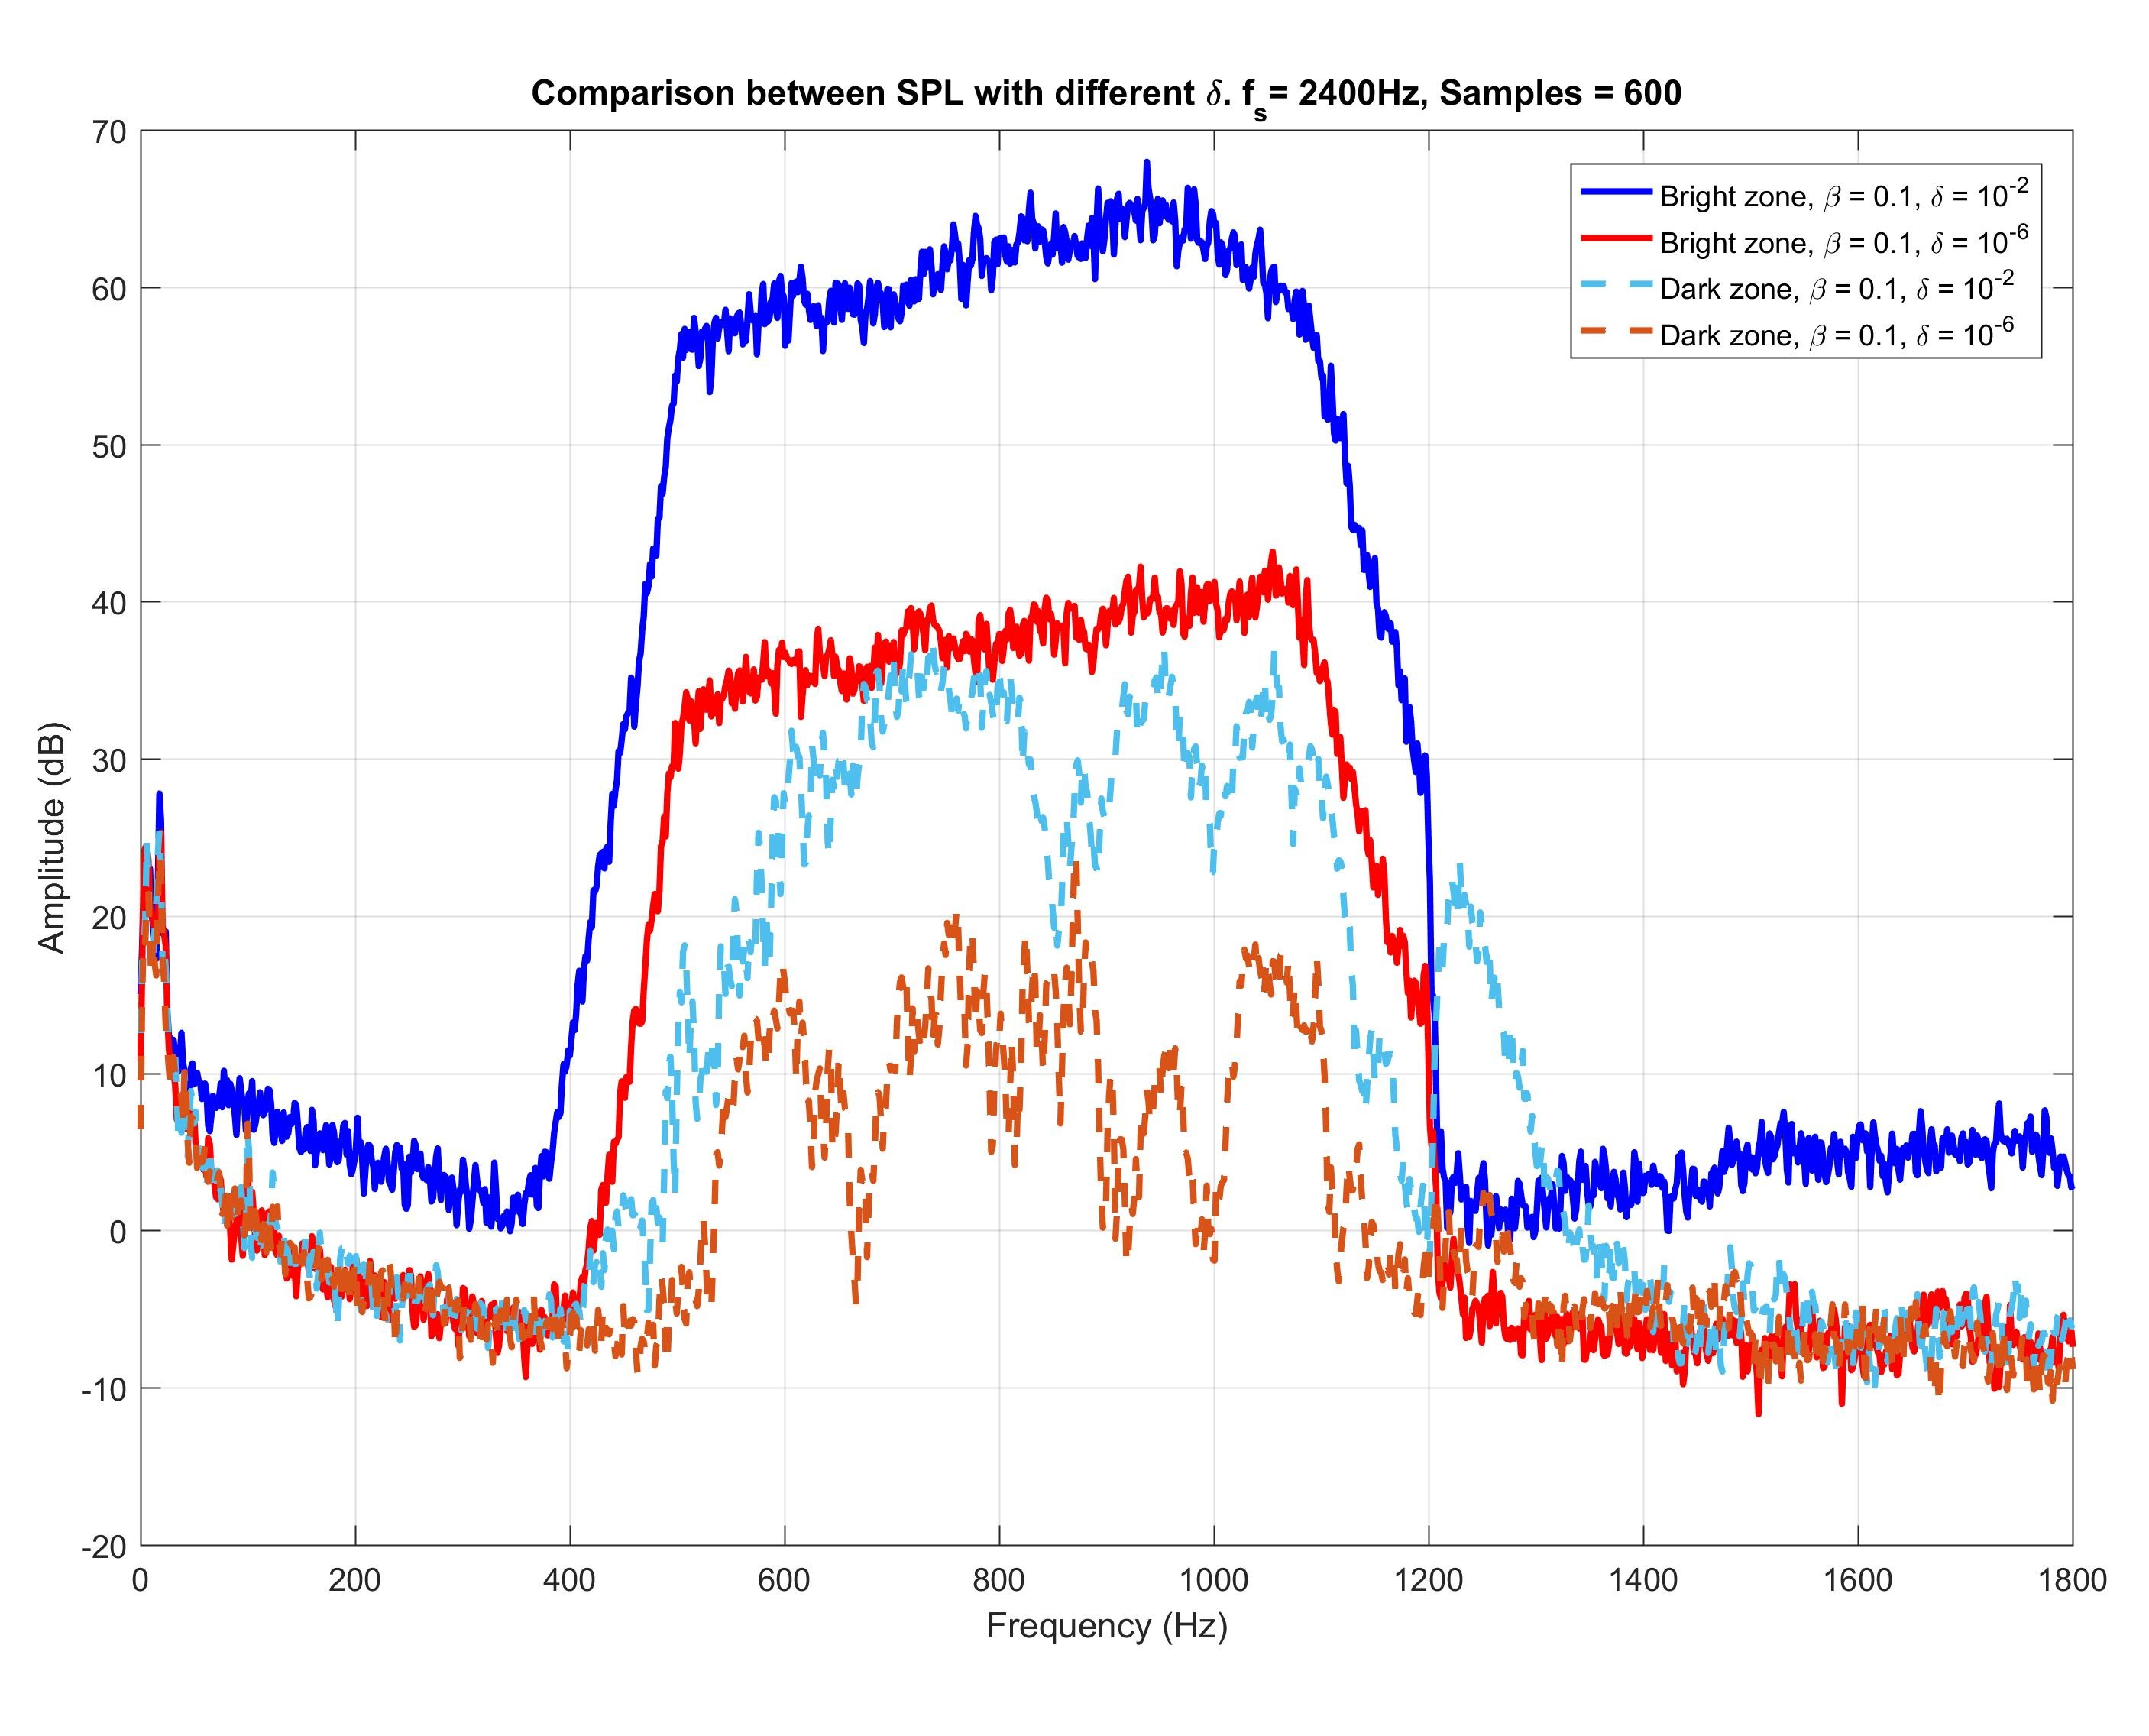
\includegraphics[width=14.5cm,height=15cm,keepaspectratio]{Figures/filter_5vs25}
\decoRule
\caption[FFT filters same beta]{FFT of the recording of microphone 20 for two filters with different $\delta$.}
\label{fig:filter_5vs25}
\end{figure}

As shown in the figure, even though a value of $\beta = 1\text{x}10^{-2}$ grants an higher contrast ($29.2\pm2$dB, blue vs light blue line) its behavior in the range of interest ([500-1100]Hz) is less linear compared with the filter which has $\beta = 1\text{x}10^{-6}$ ($22.2\pm2$dB, red vs light orange line), meaning that the variations of SPL with regard of frequency are less predictable and the mean square distance from its mean value is bigger.
\\
\\
In the end we can say that increasing the filter length over $300$ samples is not so important, since it appears that the algorithm does a good enough job with few samples, this is probably due to the "easy" test environment given by the anechoic chamber, which has a relatively short IR.

\subsection{Splitting the system Impulse Response}{}
\label{subsec:filtersplit}


We have looked at the algorithm and the effect that changing some parameters have. We will now add a reflection source in the anechoic chamber, such as the one described in section \ref{subsec:reflector} and draw some conclusions.
\\
The panel is situated at $1$m from the microphone matrix and $30$cm to the right from the center of the second speaker array, roughly behind the bright zone, the rest of the setup is identical as the one presented in figure \ref{fig:anechoicsetup}.
We can see what kind of effect such an object has, when estimating the system impulse response, by using the Logsweep method.

\begin{figure}[H]
\centering
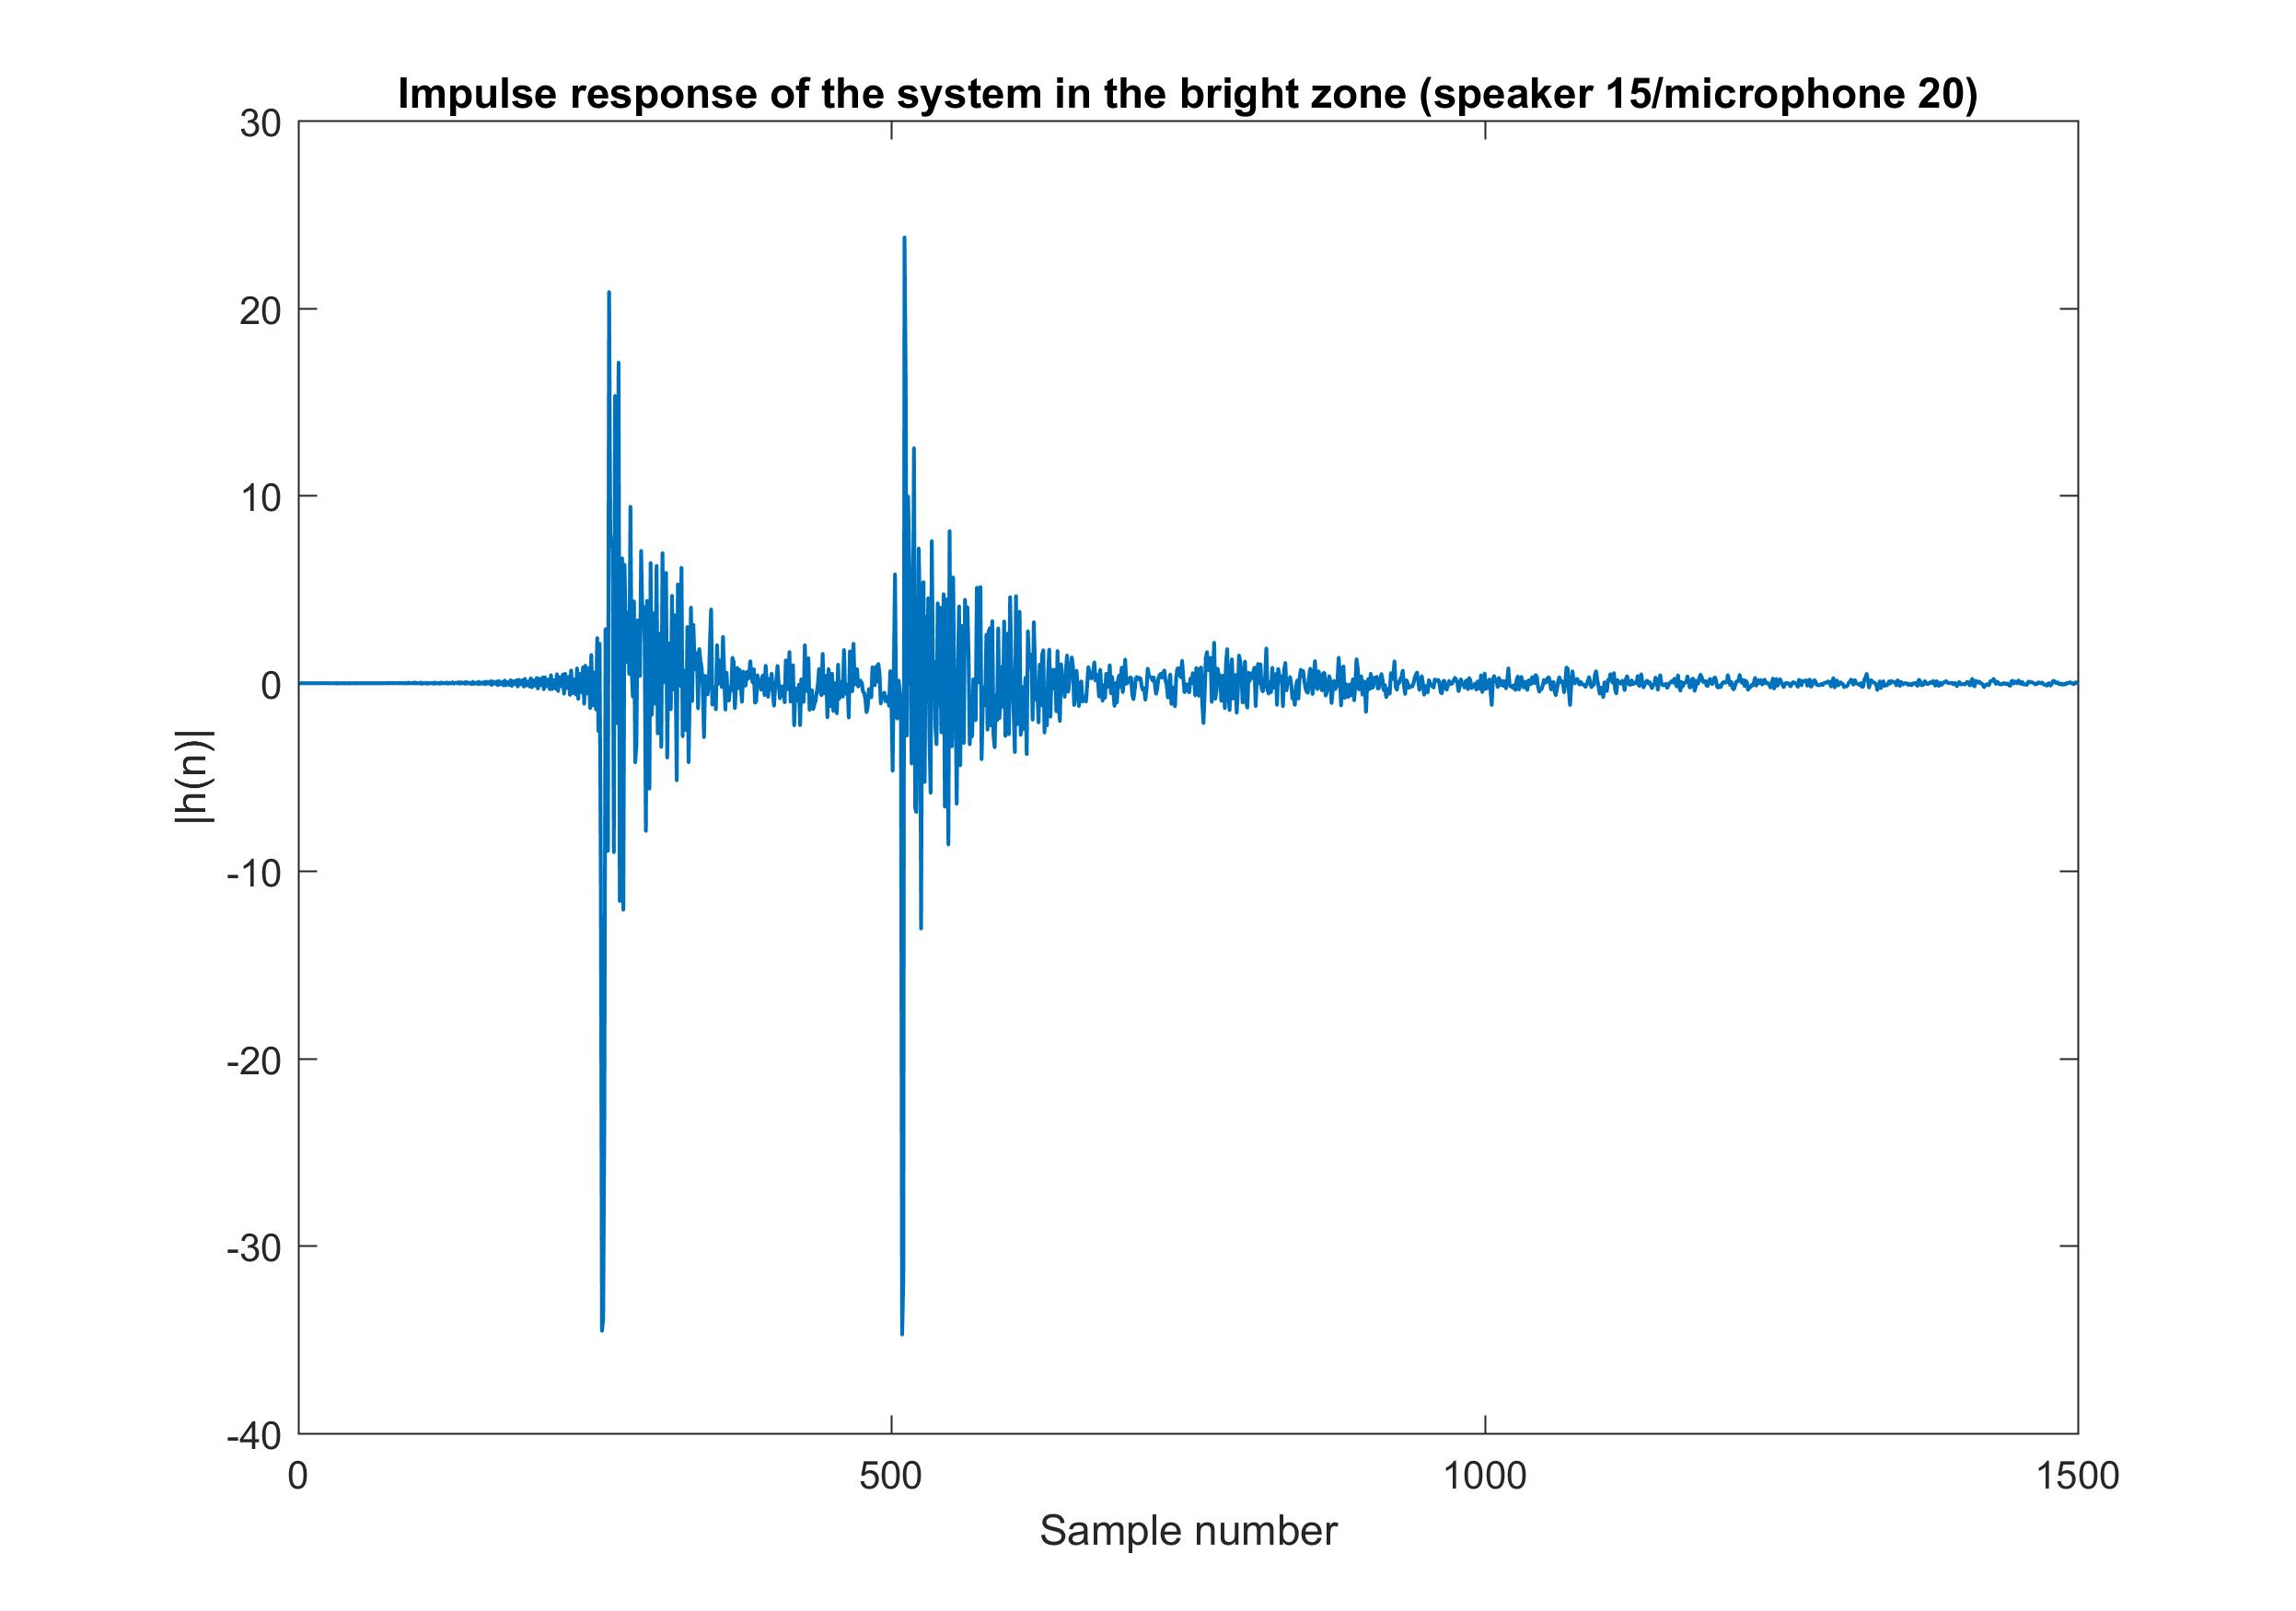
\includegraphics[width=15cm,height=15cm,keepaspectratio]{Figures/ir_refl_bright}
\decoRule
\caption[Impulse response]{Impulse response of the system.}
\label{fig:ir_refl_bright}
\end{figure}

The second peak from the left in the IR represents the soundwave being reflected by the panel and hitting the microphones, after it had passed them a first time (represented by the first peak, which corresponds to the hit of the direct wave). The reader can compare the IR presented above with the one in figure \ref{fig:ir_bright}.
\\
The distance between the two peaks is strongly tied with the position of the reflector, the more distant it is from the microphone matrix, the later (higher in sample number) the peak will appear. Moreover, we can notice a longer tail in the IR, this means that more samples (moving to the right of the graph) will now have some information content. In other words, we need more samples to represent the system with a relative accuracy and ignoring the long tail when running the ACC algorithm will lead to a decrease in the contrast figure.
\\
\\
Rerunning the experiment of section\label{subsec:baccrdanechoic} (the first one in the anechoic chamber, with the same parameters of $\beta=0.5$, $\delta=1\textbf{x}10^{-6}$, same filter and IR length $M=I=400$ and $-35$ of volume in relative scale), we can see the contrast figure be reduced to $20.6\pm2$dB (compared to $24.5\pm2$dB of the first experiment, the one without the reflector).
\\
This is because of two reasons. First and more importantly, the reflection source introduces more energy to the room, it redirects soundwaves that have already passed the control zones, back towards said areas, both for the controlled and the non-controlled (higher harmonics) frequencies. This is effectively increasing the amount of nonlinear distortions present in the soundzones at a given time, reducing the contrast.
\\
The second consequence having the surface in the room has, is to increase the length of the IR necessary to have a good estimation of the channel, as we can see from the longer tail from the graph above, cutting short the IR would lead to an unacceptable information loss. With a downsampling factor of $10$ and a filter length of $400$ samples (like the first experiment) the loss is still acceptable, so this effect is less noticeable, but if the source was to be positioned further back, or if we would have defined a shortened filter vector (maybe because we wanted to decrease the computational time), we would have incurred in noticeable worsening of the contrast figure.
\\
\\
The idea of shortening the filter length is particularly interesting, since the algorithm, as it stands, it's too heavy to run on any other machine other than high performance, multi-core CPUs and even in that case it requires minutes, if not hours, to come up with the correct weights vector that constitutes the solution to the Lagrange problem \ref{eqn:lagrange}.
\\
\\
Ideally, we would like to shorten the filter length, without compromising the contrast figure.
\\
The fundamental idea behind the solution for this problem is made possible by the fact that the filter length and the IR length are independent from each other. Instead of designing a long ACC filter for the system, we could find some parts, two in this case, where the IR has the most information content, those correspond to the samples in proximity of the two peaks. We could window those sections out and find a solution for each one of this parts independently. We would have two resulting filters that we could then put back together (by spacing them out accordingly) and use as one, instead of calculating the result for a single, longer filter. The computational time of this kind of solution would be in the magnitude of seconds instead of minutes or hours. The two short filters can be seen as "local" optimal solutions to the algorithm, that contrast a particular \textit{set} of soundwaves. With the word \textit{set} I mean waves that are originated (or reflected) by a same source and which arrive to the control point at relatively the same time.
\\
\\
To apply this idea we have, first of all, be able to systematically detect the peaks in the IR. In order to do that, we calculate the correlation between the loudspeakers input, which is the Logsweep signal, and the output, that is the signal picked up by the microphones. \\
One peculiarity of the impulse response of this kind of system is that the reflected wave starts showing its effect in the IR in the negative part of the graph. This is because the direction of arrival of the reflected sound is opposite to the one of the direct wave. Once the position (which here has the meaning of sample number, in figure \ref{fig:ir_refl_bright}) of the peaks can be reliably found, we can decide a windowing function to apply to each one of the two parts of the system.
\\
\\
In this case the window applied is a square function, which, unfortunately, is not a very good choice, since causes ripples in the frequency domain, but it appears that applying a more practical window (like the Blackmann window, which is more bell-shaped in the time domain, hence having a better side-lobe attenuation) has the effect of degrading the impulse response to a point where the weights vector $w_{BACC}$ is not effective anymore, since essentially is based on an IR that is too distorted, and not representative of the system under test.
\\
This appears to be a drawback of applying windowing to signals that have too few samples. The windowing problem will surely need some more studying to really improve the applicability of this method in a less-than-ideal scenario. In any case, since the frequency of the test signal is limited in a relatively short range, the contrast figure and the frequency response of the filter is affected by the square function in an acceptable (even though suboptimal) way. 
\\
The algorithm automatically detects the starting and ending point of the windows, so that the two filters can be merged correctly. A series of 0-valued elements are added in between the two windows (if needed) to correctly align the two parts of the system.
\\
\\
Unfortunately it appears that the reflector surface used for the tests was ill-suited for this kind of experiment. Even though its effect is pretty visible in the impulse response \ref{fig:ir_refl_bright}, when measuring the SPL, it appears that the amount of energy added in the soundzones by the presence of the panel is too low to be significant. Specifically, when putting the microphone matrix in the bright zone and measuring the SPL (in a similar fashion to what has been done for section \ref{subsec:speakers}) the result was an increase of $0.5$dB (from $89.9\pm0.2$dB to $89.4\pm0.3$dB). One more interesting property of the new system can be found in the frequency response

\begin{figure}[H]
\centering
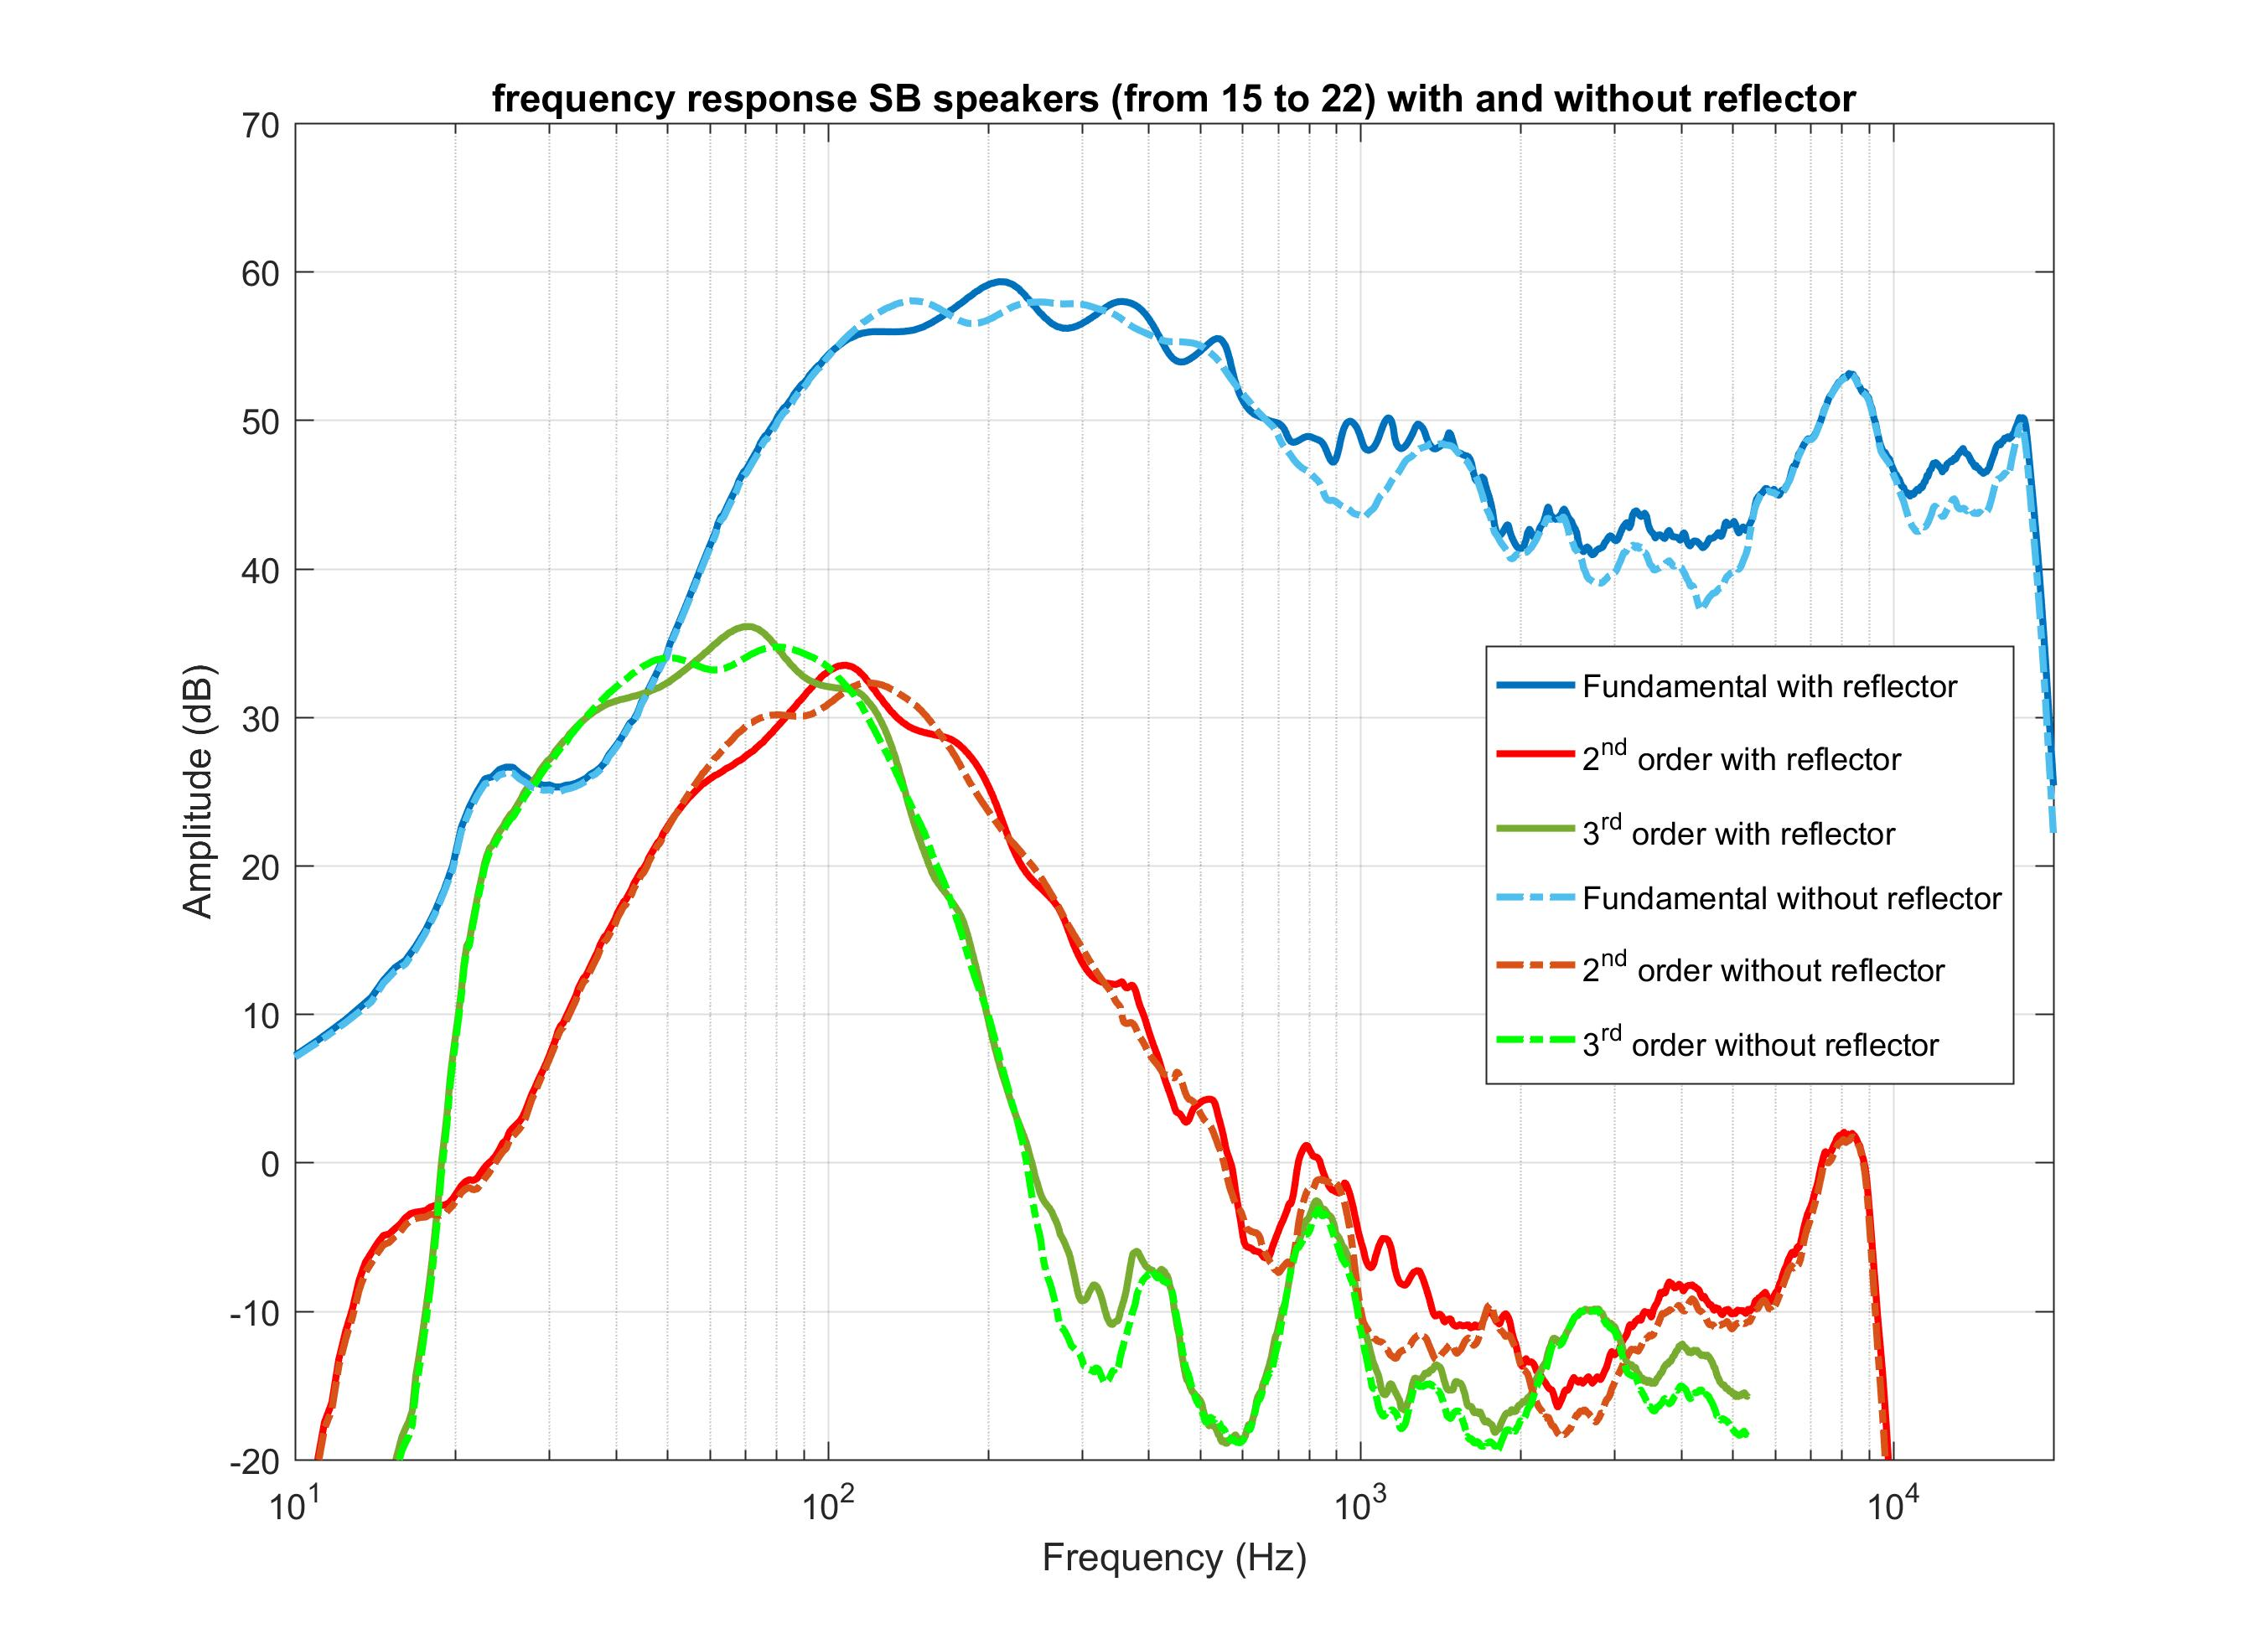
\includegraphics[width=15cm,height=15cm,keepaspectratio]{Figures/sbwithwithoutfreq}
\decoRule
\caption[Frequency response with and without reflector]{Frequency response of the system with (solid lines) and without (dotted lines) reflector.}
\label{fig:freqrespwithwithout}
\end{figure}

It appears that, when the reflector is inside the chamber, the amplitude of the harmonics starts oscillating. This is caused by the standing wave effect. The reflected waves have a certain phase when arriving at the detection point. Depending on the phase value, those have the effect of lowering or increasing the amplitude of the direct wave, since they interfere with each other. As it can be seen from the graph, the magnitude of this phenomena is too weak to cause a significant effect on the frequency response (even though it is clearly visible) and by extension on the ACC filter coefficient estimation.
\\
The $w_{BACC}$ filter calculated with the modified BACC-RD method is presented below. The black box represents a closeup of the second part of the filter. Its ratio is 70:1 with respect of the original scale.

\begin{figure}[H]
\centering
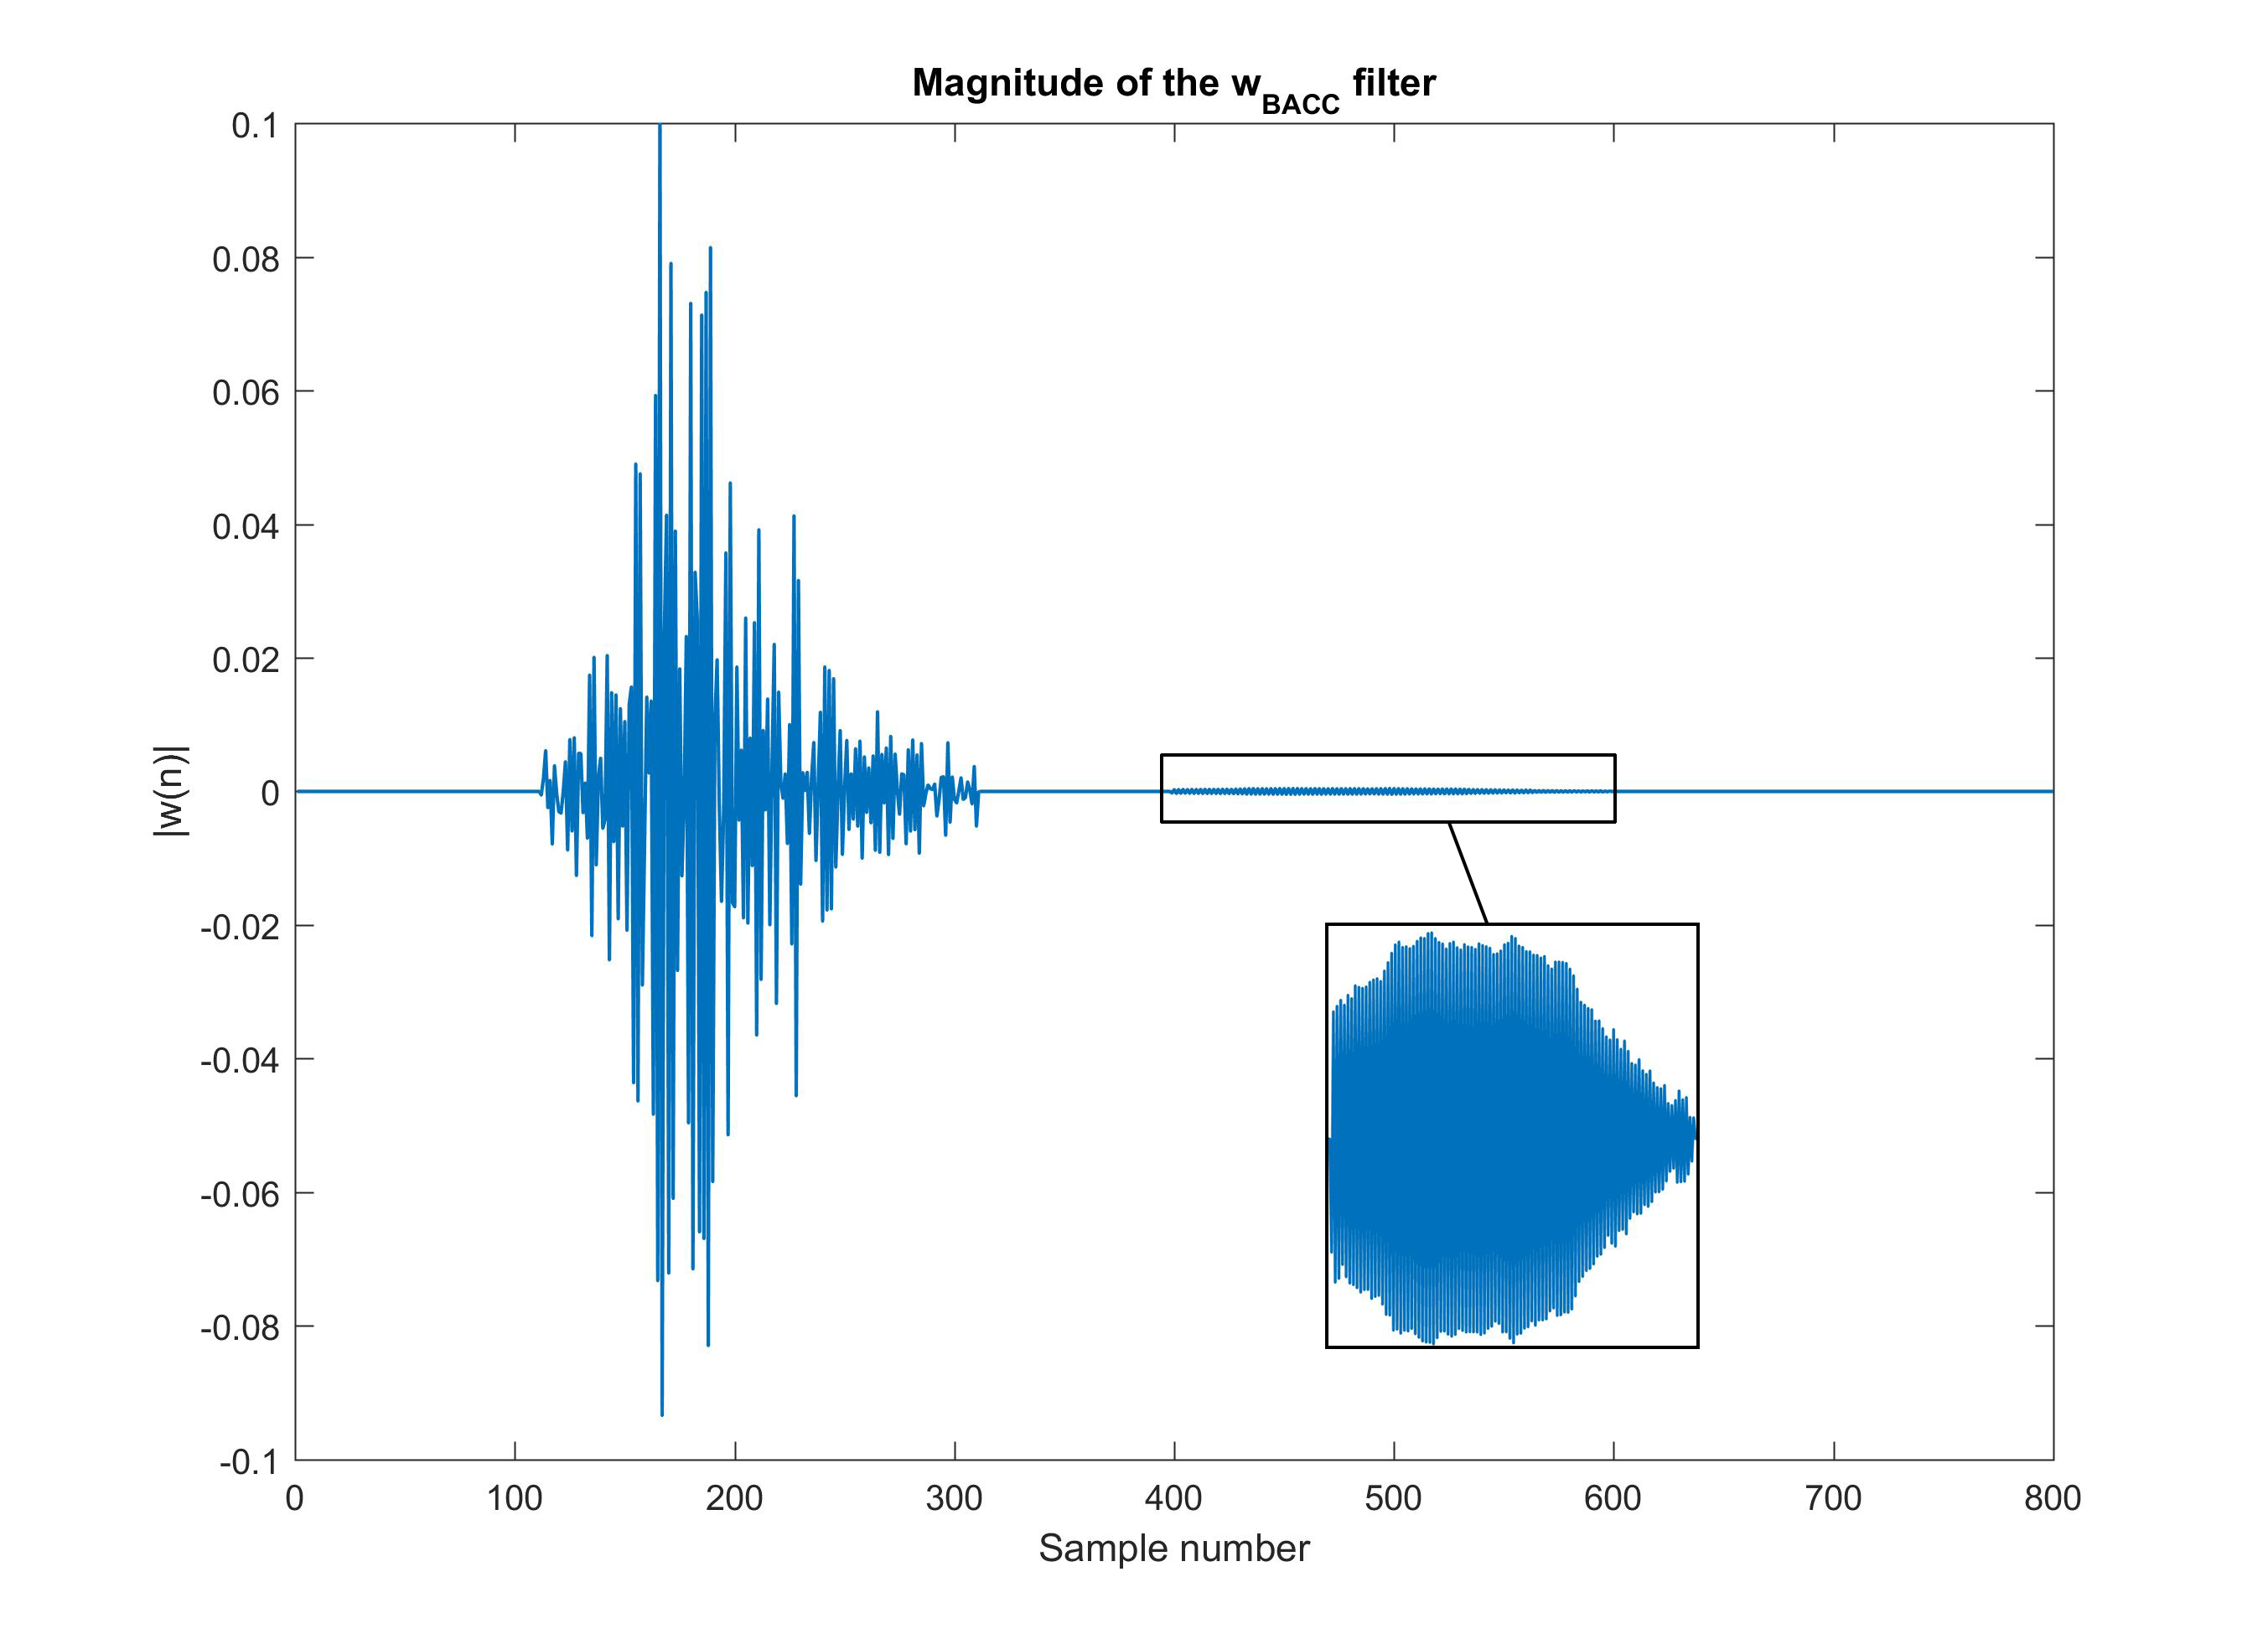
\includegraphics[width=14cm,height=14cm,keepaspectratio]{Figures/filtersplitwithcloseup}
\decoRule
\caption[filter split]{Optimal solution to the Lagrange problem, the black box represents a closeup of the second part of the solution.}
\label{fig:filtersplitwithcloseup}
\end{figure}

As we can see from the final result of the Lagrange problem the part of the filter that contrasts the reflection has an amplitude that is too low compared with the first part of the filter, this is because the energy of the reflected wave itself is too low compared with the one of the direct wave. Nevertheless we can measure the contrast generated by this filter.
\\
\\
Here we can see the frequency response of the system as recorded by microphone $20$. The regularization terms used were $\beta=0.5$, $\delta = 10^{-6}$, an output level of $-35$ and input signal in the $[500-2200]$Hz range. The Contrast figure is $21.8\pm2$dB, obtained by averaging five trials of the experiment.

\begin{figure}[H]
\centering
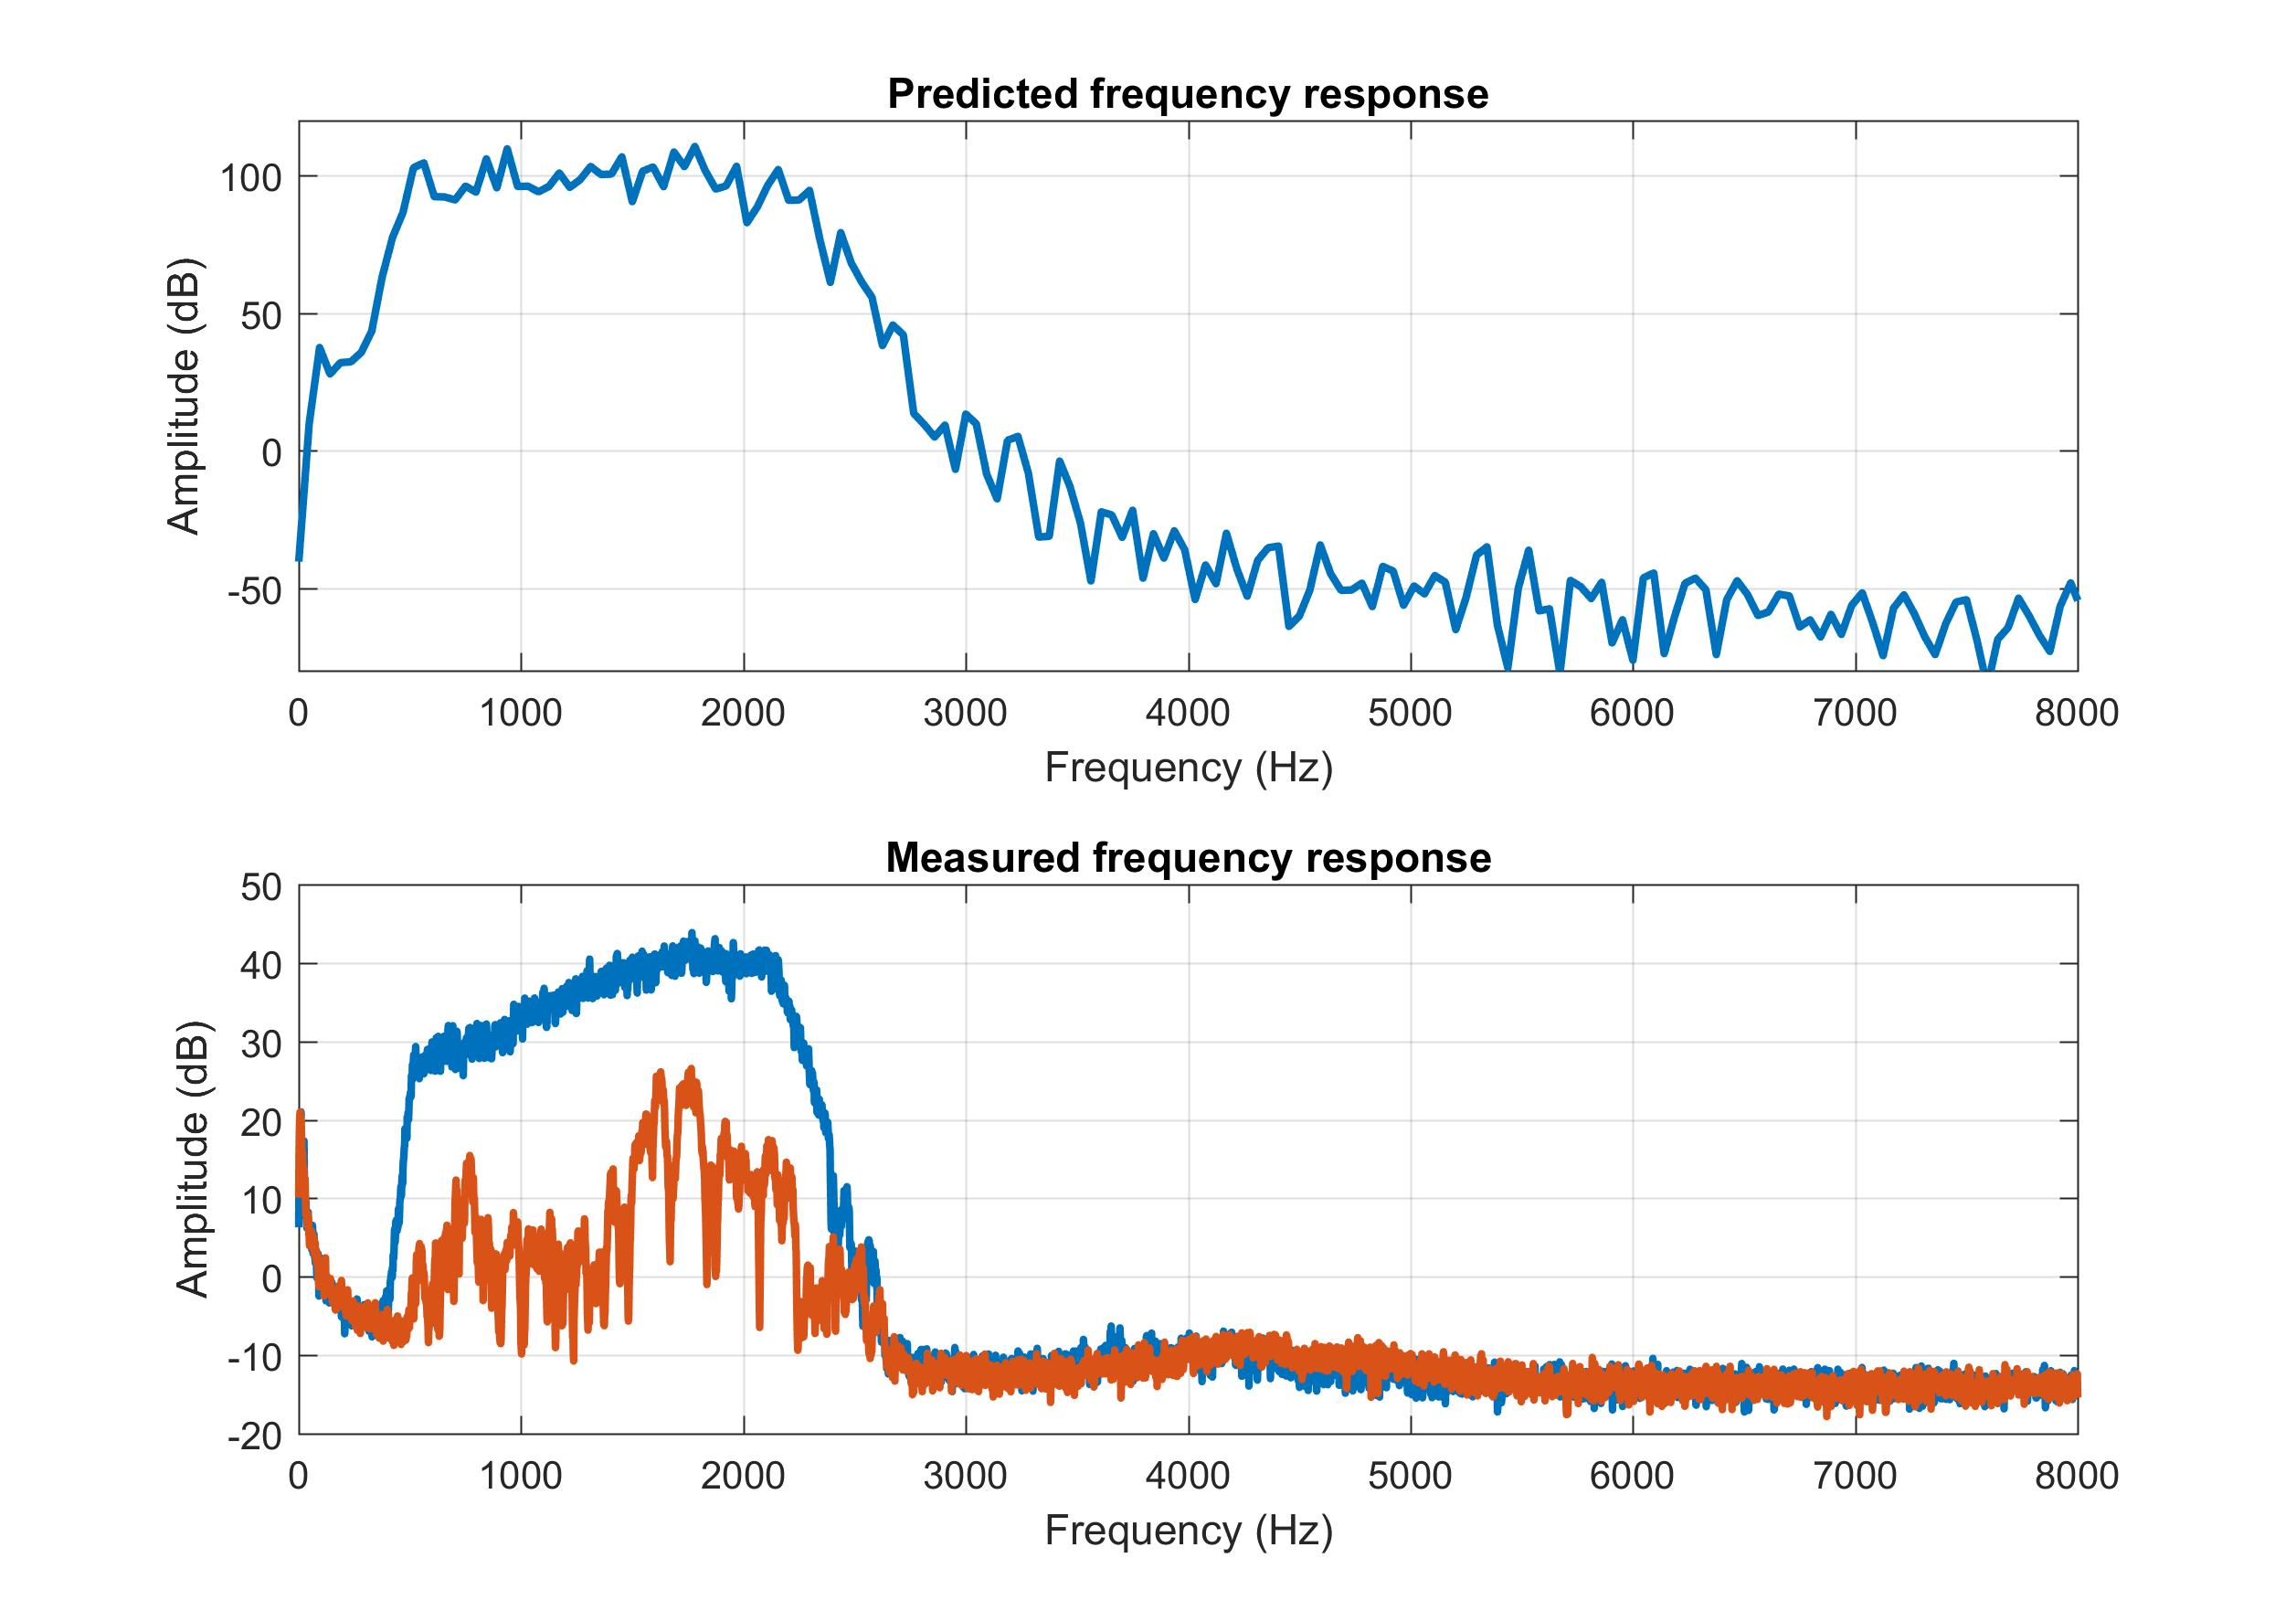
\includegraphics[width=15cm,height=15cm,keepaspectratio]
{Figures/fftbaccsplit}
\decoRule
\caption[Frequency response]{Frequency response of the system when applying the filter in figure \ref{fig:filtersplitwithcloseup}.}
\label{fig:welchfiltersplit}
\end{figure}

The total filter length of 400 samples, divided in two pieces of 200 samples each. The system IR from which the filter was calculated (a cut out of the IR represented in figure \ref{fig:ir_refl_bright}) was 800 samples. The sampling frequency, downsampling rate, microphones and speakers used are the same of the experiment done with a single filter. Is it therefore natural to compare this contrast figure with the one in the experiment \ref{subsec:baccrdanechoic}, an attentive reader will notice the similarity between the spectra of the two graphs (\ref{fig:fr_multiple}).
\\
The contrast figure obtained in that section was $24.5\pm2$dB. The contrast obtained by a BACC filter obtained with the same algorithm of section \ref{subsec:baccrdanechoic}, granted $20.6\pm2$dB, as explained at the beginning of this section. The modified version of the algorithm gives us $21.9\pm2$dB of contrast. It is reminded that all of the measurements have been repeated five times and the results averaged. As we can see the improvement is very modest and generally it has be said that even though encouraging, this solution here proposed requires more studying order to evaluate its efficacy. The algorithm is a good starting point when it comes to tackling the reflection problem in a simplified scenario such as the one used for the experiment.
\\
\\
The reader should be made aware of the shortcomings of the algorithm. First of all, it is clear that the second part of the filter affects the system in a limited way. This is due of the low energy that the reflector adds to the sound zones. One interesting development of this experiment would be to execute the algorithm with a different reflector, possibly one with a more visible effect than the one currently available. Moreover, as previously said, the square window is a suboptimal window function that can affect the system in a negative way.
\\
Due to these limitations it is hard to say that this modified version has a clear beneficial effect to the overall contrast and though it certainly it has not a negative impact in the contrast, more research is needed to study its potential positive effects.


\section{Bacc-RD in the listening room}{}
\label{sec:baccrdlisteningroom}

In the previous section we investigated the characteristics and performances of the BACC-RD algorithm in an anechoic chamber setup and explored a possible modification that can be applied to the concept in a scenario with a single reflector.
\\
Let's now consider a different environment, the listening room. We already presented the setup of the room in section \ref{subsec:mics} and discussed that by its nature, this scenario it's much more difficult to control, since there asre many surfaces that scatter the sound energy everywhere.
The figure below shows the impulse response of the room in question

\begin{figure}[H]
\centering
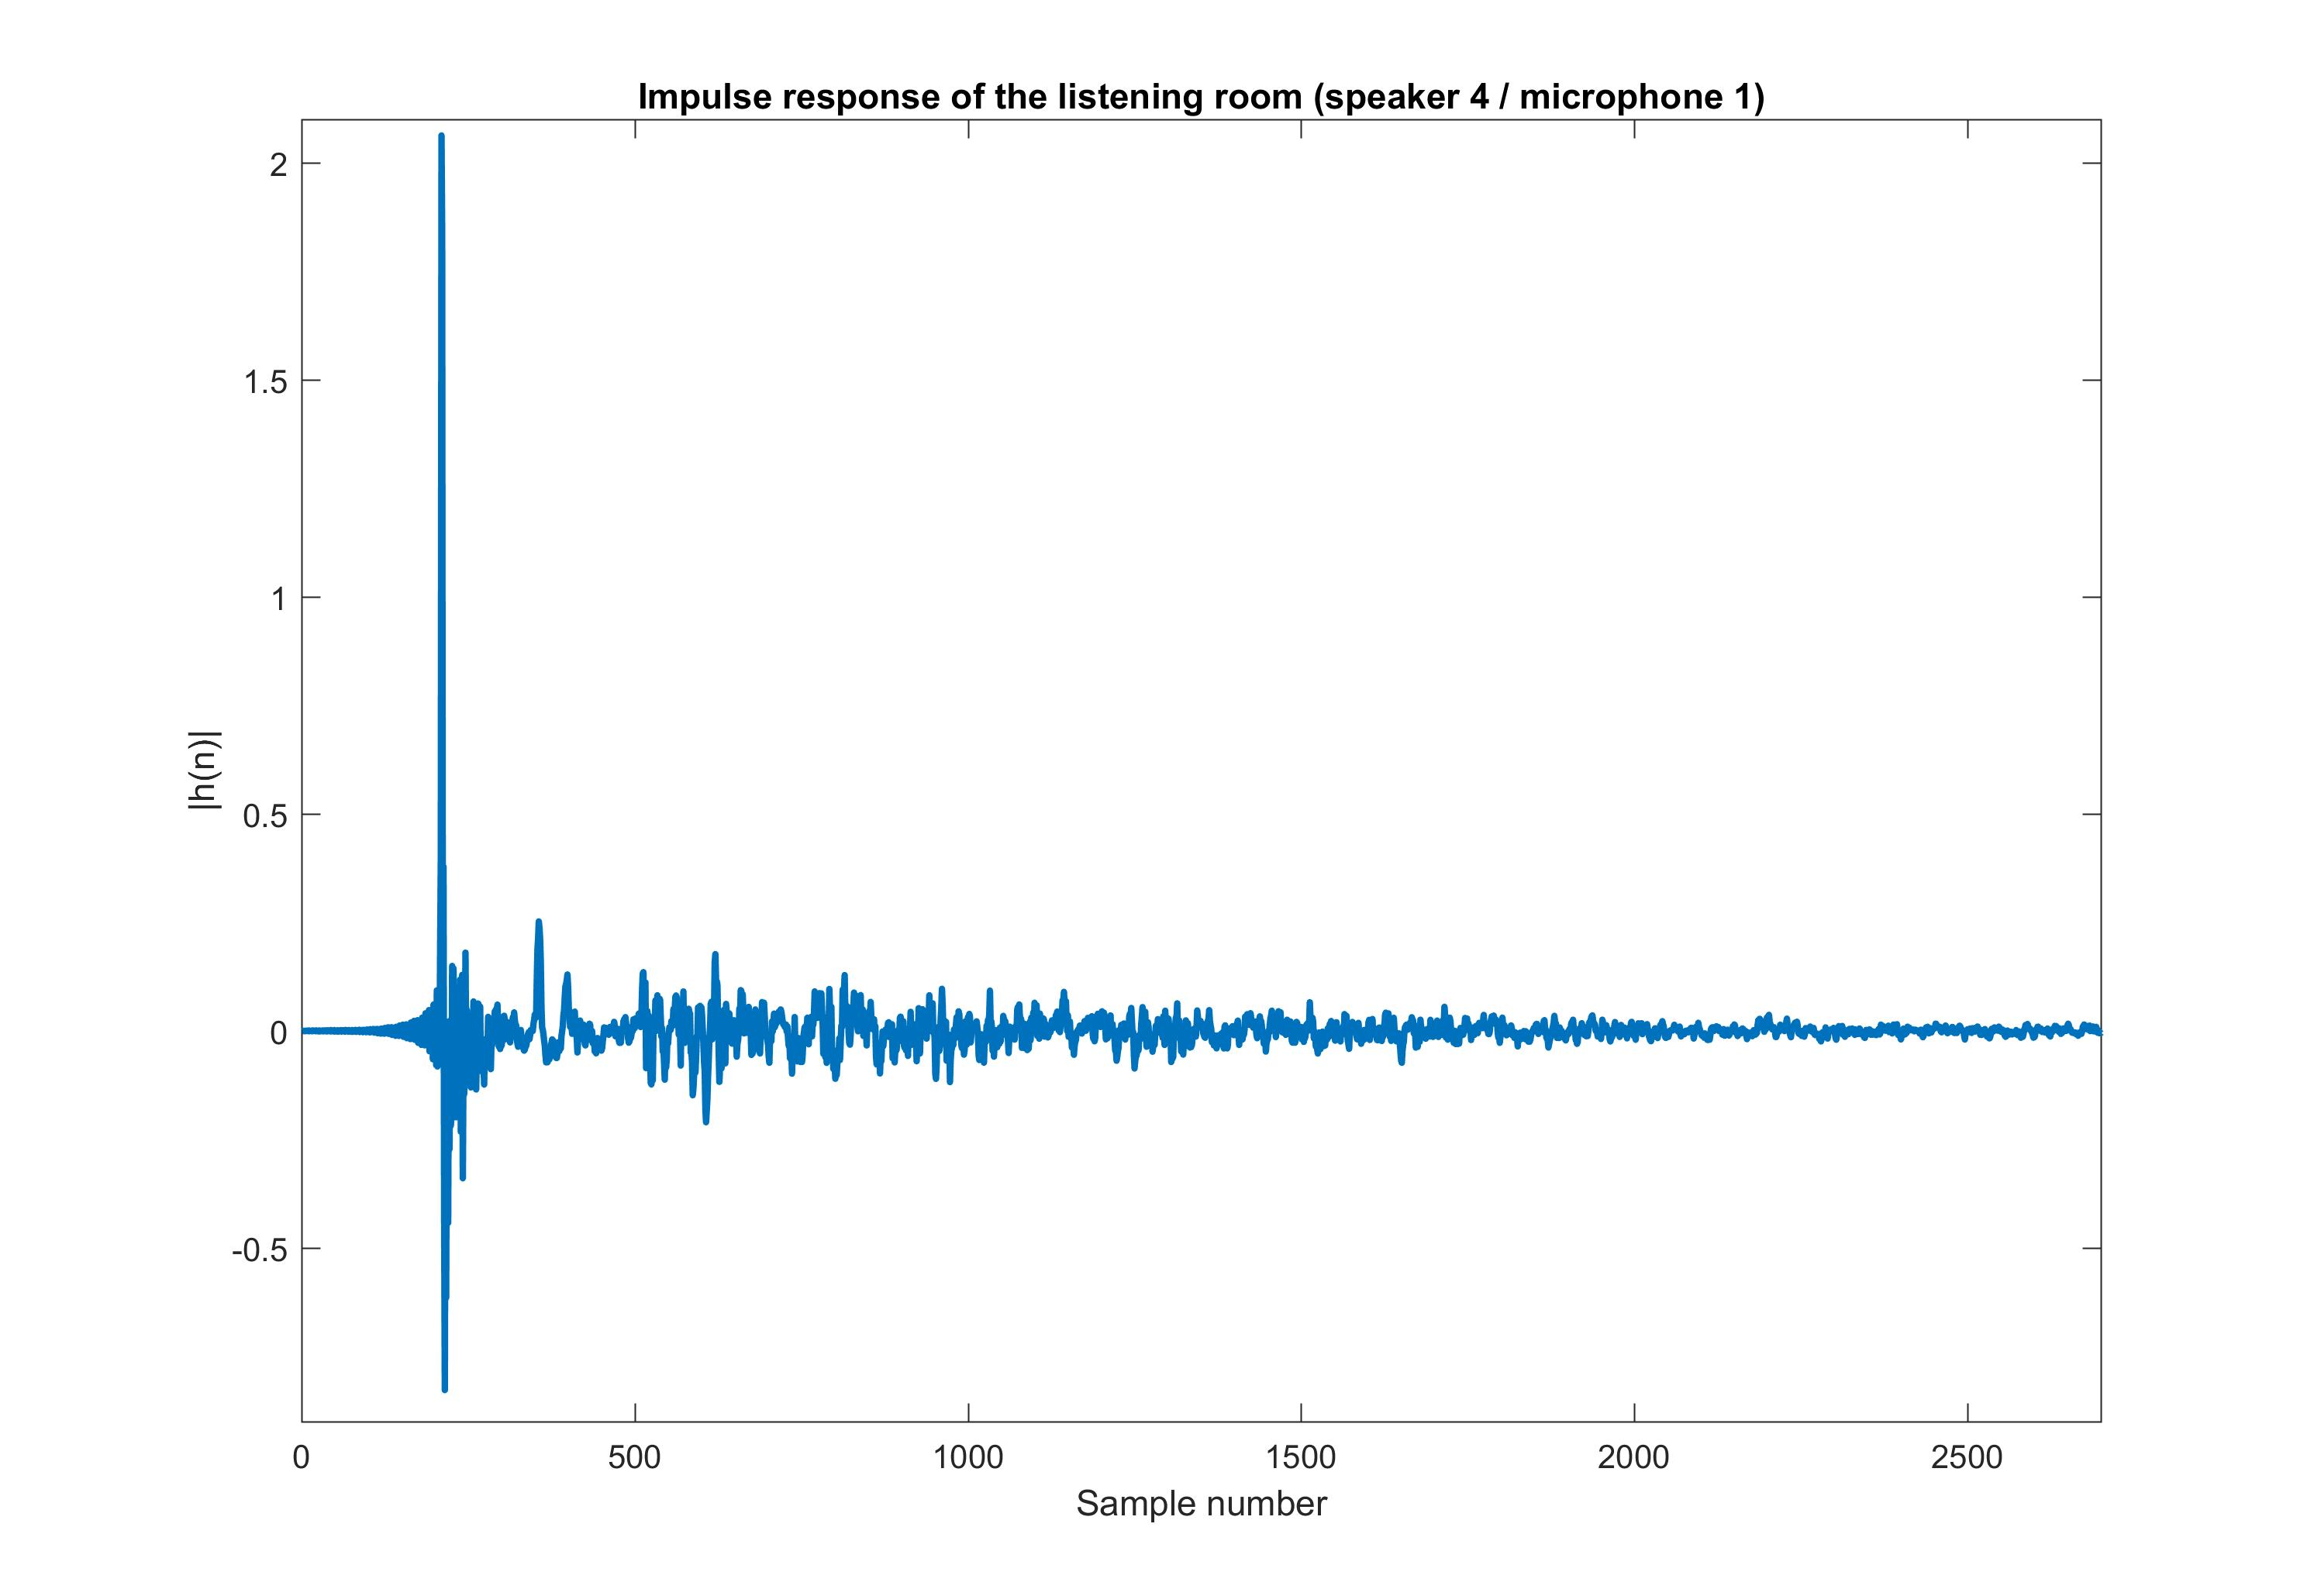
\includegraphics[width=15cm,height=15cm,keepaspectratio]
{Figures/irlisteningroom}
\caption[IR listening room]{Impulse response of the listening room detected in the bright zone.}
\label{fig:irlisteningroom}
\end{figure}

As we can see, in order to represent the system effectively, we need many samples of the IR. Since this introduces unacceptable computing times, especially for the $R_b, R_d$ terms in equation\ref{eqn:lagrange}, we need to limit as much as possible the filter length
\\
The room setup is shown in figure \ref{fig:listeningsetup}. While recording the room's impulse response and performing the test I am inside the room.
\\
Using the original filter concept (the one in sections \ref{subsec:baccrdanechoic} and \ref{subsec:baccvary}) we get a contrast figure of $13.1\pm2$dB, using a $400$ taps filter with $\beta = 0.5, \delta = 1\text{x}10^{-6}$ and a frequency band in the $[500-1800]$Hz range.
Some things have to be said for this figure, first of all the actual contrast detected by each microphone has much more variance, meaning that even though the average figure is the one stated above, some microphone show a contrast as low as $10$dB, while other have a contrast of $16.5$dB. This is due the standing wave effect, which, as we already explained, is a phenomena generated when a soundwave that is reflected back to a given position interferes with another wave coming from a different direction, this generates destructive or constructive interferences at some given positions (dependent on the wave length of the waves) called nodes. The resulting wave is generated by a superposition of the two, which means that will have an amplitude, phase and direction which depends by the characteristics of the interfering sounds.
\\
\\
Due to the spatial dependency of the standing wave effect, the individual regularization of the speakers weights ($\beta, \delta$) might once again prove to be beneficial for the contrast figure.
\\
\\
Using the new algorithm with the same parameters ($400$ taps, $\beta = 0.5, \delta = 1\text{x}10^{-6}$) leads to a contrast $15.4\pm2$dB, which is a modest improvement on the result achieved by the original version of BACC-RD. This is given by the fact that the algorithm automatically detects the source that contributes most to the reflections, by calculating the correlation between the logsweep signal before and after being outputted from the speakers.
\\
The following figure presents the frequency response of the system when solicited with the filters discussed above, the first graph shows the FFT of the recorded samples when the original BACC-RD has been used to find the weights vector, while the second shows the performances achieved with the modified algorithm.

\begin{figure}[H]
\centering
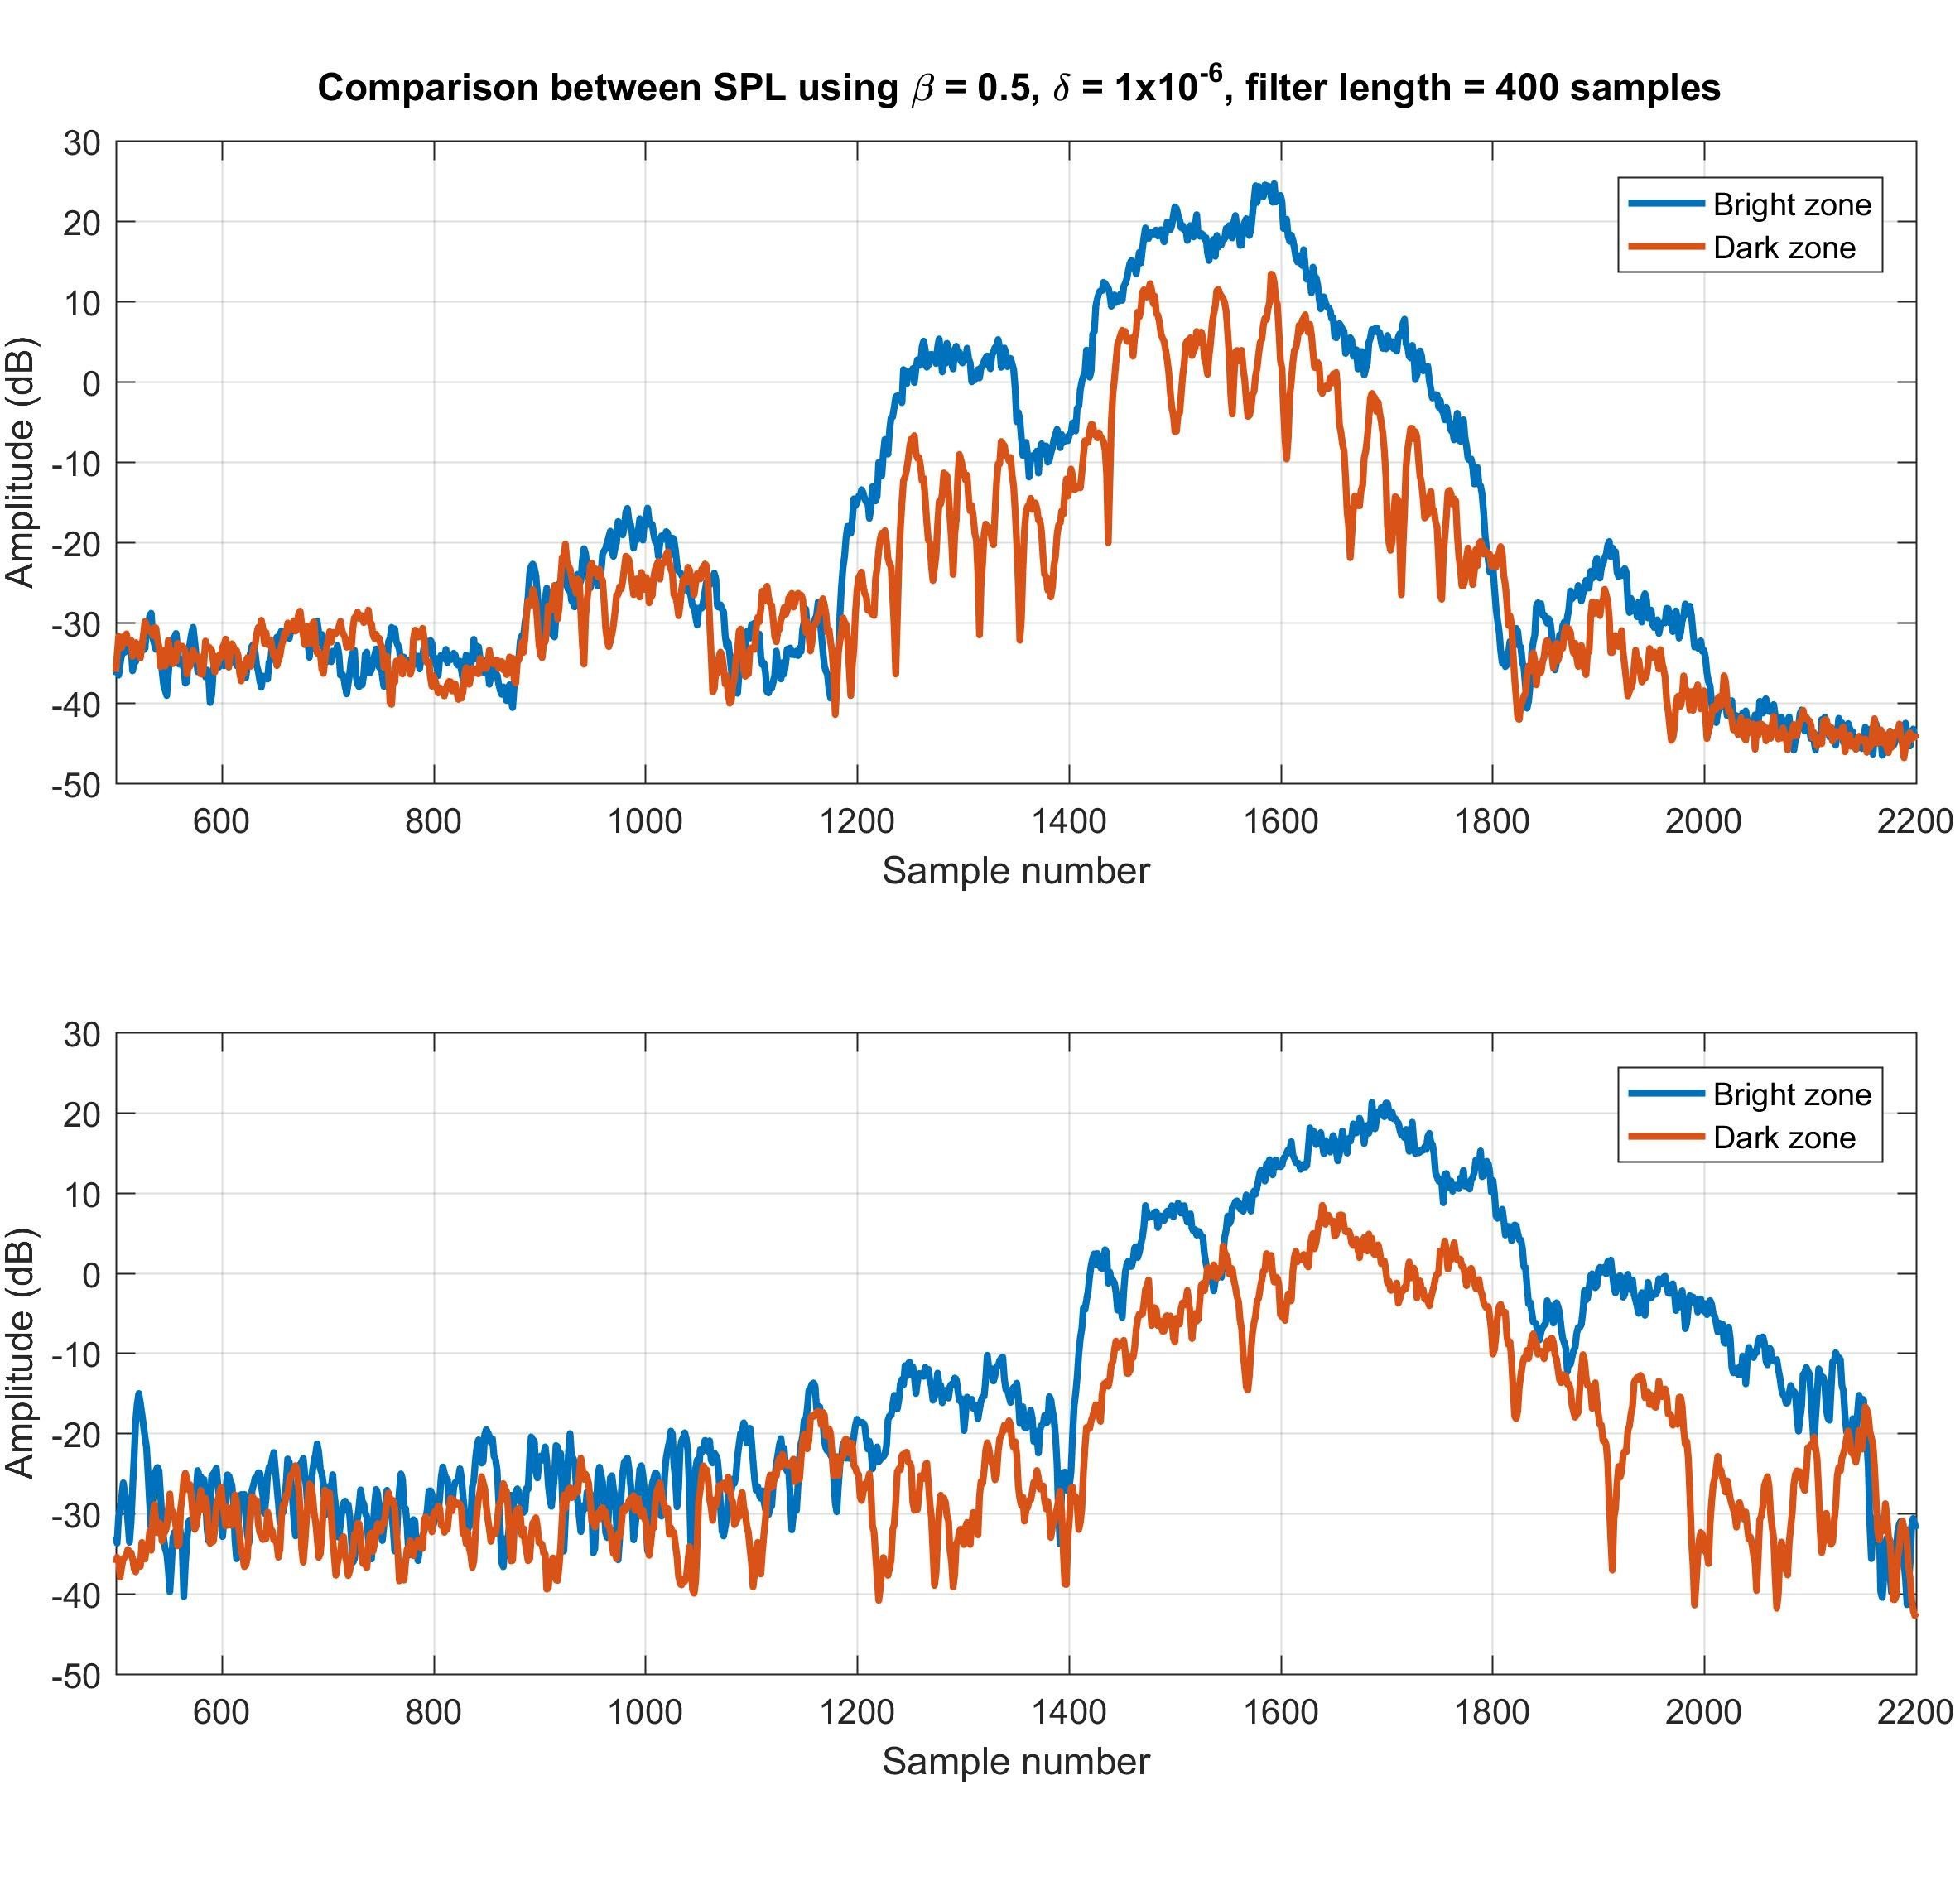
\includegraphics[width=15cm,height=15cm,keepaspectratio]
{Figures/fftfilterslisteningroom}
\decoRule
\caption[FFT listening room]{Fast Fourier Transform of the samples recorded in the listening room using the two verisons of the BACC algorithm.}
\label{fig:fftfilterslisteningroom}
\end{figure}

As we can see the energy is totally concentrated close to the upper frequency limit of the signal. This kind of behavior generates too much distortions of the original sound signal. This graph shows that introducing a new constraint regarding the difference in power level that can be allowed to two adjacent frequency bands seems to be even more beneficial in this kind of environment than the one of the anechoic chamber.
\\
We can also see how the signal, once convolved with the filter, loses almost all its lower frequency content, which doesn't reach the $0$dB mark before $1400$Hz. This kind of behavior is justifiable by the fact that having short filter length means that the algorithm is more capable of controlling only the higher frequencies, for instance, since we have a $400$ taps filter (in the first graph) and a sampling frequency of $4800$Hz the theoretical limit that can be controlled is $\frac{4800}{400}=12$Hz. In the second case we have an even higher theoretical limit, since we split the IR (and the filter) in two parts of $200$ taps each. We can in fact see how the modified algorithm (in the second graph) "pushes" the signal to the higher frequencies even more than the first filter.
\\
\\
Increasing the filter length generates an improvement of contrast, in fact, using $500$ taps we have a jump of \tld$2$dB in the contrast figure. In this case, unlike section \ref{subsec:baccvary}, the filter length is an important parameter to take into account, keeping in mind that the computational time greatly increases for longer filters (\tld 6 minutes for a $500$ taps, \tld1 hour for $600$ taps).
The contrast figure of the new algorithm, instead, seems not to scale with increasing the filter length, because the two "pieces" of the filter tend to end up adjacent one another, and at that point the original algorithm is superior because the control frequencies that determine the local maximum of the contrast are more tightly spaced one another, since they depend on the filter length (so they are at half the distance in a $500$ taps filter rather than 2 partial filters with $250$ taps each.
